%\documentclass[AER  , draftmode]{AEA}
\documentclass[11pt, a4paper]{article}
\usepackage[nohead]{geometry}
\geometry{left=1in,right=1in,top=1in,bottom=1in} % set margins


\usepackage{soul}
\usepackage{natbib}
\usepackage{graphicx}             
\graphicspath{{./paper/Figuras/}}
\usepackage{hyperref}

\usepackage{float}                
\usepackage{amsmath}
\usepackage{amscd}
\usepackage{amsfonts}
\usepackage{amssymb}
\usepackage{bbm}
\usepackage{booktabs}
\usepackage{nameref}
\usepackage{multirow}
\usepackage[nokeyprefix]{refstyle}
\usepackage{rotating}
\usepackage{threeparttable}
\usepackage{lscape}
\usepackage{enumerate}
\usepackage{afterpage}
\usepackage{caption}
\usepackage{subcaption}
\usepackage{epstopdf}
\usepackage{comment}


\epstopdfDeclareGraphicsRule{.tiff}{png}{.png}{convert #1 \OutputFile}
\AppendGraphicsExtensions{.tiff}

\epstopdfDeclareGraphicsRule{.tif}{png}{.png}{convert #1 \OutputFile}
\AppendGraphicsExtensions{.tif}

\usepackage{tikz}
\usetikzlibrary{shapes.geometric, arrows}
\usetikzlibrary{calc}

\usepackage{colortbl}

\newtheorem{theorem}{Theorem}
\newtheorem{claim}[theorem]{Claim}



\usepackage{anyfontsize}
\usepackage{float}
\usepackage{placeins} %esto es solo para poder 
%%% HELPER CODE FOR DEALING WITH EXTERNAL REFERENCES
\usepackage{xr}
\usepackage{setspace}
\usepackage{caption}

\makeatletter
\newcommand*{\addFileDependency}[1]{
  \typeout{(#1)}
  \@addtofilelist{#1}
  \IfFileExists{#1}{}{\typeout{No file #1.}}
}
\makeatother

\newcommand*{\myexternaldocument}[1]{
    \externaldocument{#1}
    \addFileDependency{#1.tex}
    \addFileDependency{#1.aux}
}

\myexternaldocument{OA}
\doublespacing

% -------------------------------------------------------------------------------------------------------------------------------------------------------------------

\begin{document}


\title{Information and Bargaining through Agents: Experimental Evidence from Mexico's Labor Courts}

%\shortTitle{Information and Bargaining through Agents}

\author{Joyce Sadka,  Enrique Seira, and Christopher Woodruff  \thanks{\protect\linespread{1}\protect\selectfont Sadka: ITAM, jsadka@itam.mx;  
Seira: ITAM, enrique.seira@itam.mx; Woodruff (corresponding author): University of Oxford, Department of International Development, Oxford OX13TB, UK, christopher.woodruff@qeh.ox.ac.uk. Acknowledgements: We would like to thank Sebastian Garcia, Andrea Fernandez, Sergio Lopez-Araiza, Enrique Miranda, Isaac Meza, Diana Roman, and Monica Zamudio for superhuman research assistance, Vince Crawford, Jonas Hjort and Bentley MacLeod for helpful discussions, and seminar and conference participants at Cambridge, Columbia, Toulouse, ITAM, Monash, NYU - Abu Dhabi, Oxford, Tinbergen, MIT/Harvard, George Mason, Maryland the Latin American Workshop on Law and Economics, and the American Law and Economics Association for comments. All errors are ours. We acknowledge financial support from the Government Partnership Initiative of the Abdul-Latif Jameel Poverty Action Lab (JPAL) at the Massachusetts Institute of Technology, the Economic Development and Institutions program funded by the UK government through UK Aid, and the Asociacion Mexicana de Cultura. We also acknowledge crucial institutional, operational, and human resource support from the Mexico City Labor Court and its president, Darlene Rojas Olvera. The research reported in the paper was carried out with the approval of the ITAM Institutional Review Board. Phase 3 of the experiment is registered as AEARCTR-0002339.}}


\date{\today}

%\pubMonth{February}
%\pubYear{2020}
%\pubVolume{ }
%\pubIssue{ }

\maketitle

\begin{abstract} Well-functioning courts are essential for the health of both financial and real economies. Courts function poorly in most lower-income countries, but the root causes of poor performance are not well understood. We use field experiments with ongoing cases to analyze sources of dysfunction in Mexico's largest labor court. Providing both parties with personalized outcome predictions nearly doubles settlement rates and reduces average case duration, but only when the worker is present to receive the information. An intervention before plaintiffs contact a lawyer increases pre-suit settlement. The experiment illuminates agency issues among plaintiffs with private lawyers. For most workers, the treatment appears to improve welfare, as measured by discounted payouts and ability to pay bills. 
\end{abstract}

\noindent Keywords: \qquad{labor courts, settlement, overconfidence, statistical information} \\
\noindent JEL Codes: \qquad{K31, K41, K42, J52, J83}





\newpage


\section{Introduction}

Well-functioning courts underpin markets and constrain private power in developed economies, but courts function poorly in most developing countries. Outcomes are unpredictable, parties are misinformed, and inefficient processes lead to slow decisions and large case backlogs  (\cite{Djankov_Courts}). In addition to raising concerns for justice, poorly functioning courts undermine both the financial (\cite{PonticelliAlencar_Bankrupcy}) and real (\cite{10.1093/qje/qjaa020}; \cite{Chemin_ReStat}) economies. 
The effects of poorly functioning courts are increasingly well documented, most convincingly through studies analyzing changes following the creation of new institutions providing judicial resolution for specific activities (\cite{Visaria_AEJAp2009}; \cite{Lichand_2014}). However, as \cite{10.1093/qje/qjaa020} note, even ``Newly created courts tend to...accumulate backlogs over time'' (p. 2009). Thus, while the existing literature provides evidence on the importance of well-functioning legal institutions, it is much less informative on how to improve the performance of existing institutions, or how to ensure the continued high performance of new institutions. This is due in part to a lack of rigorous empirical work aimed at understanding the micro-analytics of court proceedings, and a particular paucity of randomized experiments in courts (\cite{Greiner_Matthews_Review2016}).  %\footnote{One recent exception is \cite{Kondylis_Stein_Senegal}, who study the effects of an administrative reform in Senegalese courts.}


To illuminate the causes of dysfunction in courts, we conduct a randomized experiment with active cases in the Mexico City Labor Court (MCLC). In the experimental treatment, we provide parties in a random subset of labor disputes with case-specific predictions of the amount collected by the plaintiff, the duration of the case, and the probability the case ends by settlement, judgment, or by being dropped. We generate the predictions using parameters from machine-learning models run on data from 5,000 concluded cases and using variables taken from the initial case filing: daily wage, hours worked per week, tenure at the firm, whether or not the worker was registered with Social Security, and other characteristics of the position.  

The MCLC is responsible for enforcing labor law for private employers located in Mexico City. Over 95 percent of its cases involve workers who claim to have been involuntarily separated from their jobs by employers who then failed to make severance payments to the workers as required under the labor law. Dismissed workers are entitled to severance payments of a minimum of 90 days' wages and, depending on circumstances, substantially more. %are the main component of Mexico's job insurance system. 
Workers are entitled to the payments following almost any involuntary separation.{\footnote{The exception is firing for malfeasance on the part of the worker.}} The MCLC receives more than 35,000 filings each year, and had a case backlog of more than 100,000 cases at the time of our experiment. The large backlog stems from long case durations and settlement rates that are low in comparison to those of similar courts in other countries. While severance payments are a fundamental right of workers in Mexico, a national survey of workers we describe later in the paper indicates that half of dismissed workers do not receive their legally-entitled severance payment. However, only 15 percent of the workers reporting that they were not paid severance owed to them choose to pursue a claim in the court. Among the remaining 85 percent of workers, more than three-quarters said the reason for not pursuing a claim was that the court is either ``useless'' or ``too expensive.''  %First, we report data from a survey we conducted with with \# workers currently registered with the Mexican Social Security Administration (IMSS). Among the \# of workers who report being dismissed in the three years prior to the survey, 48 percent report not having received severance payments. Yet only 15 percent of those not receiving payments filed a suit in the labor court. Among the 85 percent choosing not to pursue a court case, well over half said either that the court was either ``useless'' or ``too expensive.''

Legal dysfunction has many potential sources. Our experiment holds fixed any corruption and misalignment of incentives for judges (e.g., Chemin 2020; Boehm and Oberfield 2020) and focuses instead on other potential causes of low settlement rates. We show that workers are overly optimistic and misinformed. They wildly overestimate their chances of winning their case and are not able to state basic elements of the law and even what is included in their case filing. \cite{doi:10.1146/annurev-economics-061109-080334} reviews the literature showing that overoptimism leads to delays in bargaining. \cite{Kennan_wilson} show instead that when there is asymmetric information quarreling parties use delay to communicate information, a behavior that may lead to failure to reach a settlement beneficial to both parties. While we won't distinguish between these theories, a prescription common to both is to provide objective information, which is what our information treatment was designed to do.\footnote{\cite{Kennan_wilson} argue that it may not be important to distinguish between these two causes as it is likely that overconfidence arises from parties having different information.} As most of these models predict, our treatment increases settlement rates and so decreases case duration and court congestion, while leaving plaintiffs at least as well off. However, the information has an impact only when we are able to provide it directly to plaintiffs, suggesting a third element to the story: that agency issues in the market for legal services are also a cause of low settlement rates. 


We begin by using the historical case files to document a set of stylized facts about the functioning of the court. These facts show that, while on paper labor law favors workers in Mexico, in practice the system does not work in their favor. First, workers rarely file suits even when employers fail to make severance payments, and second, the historical case file data show that plaintiffs receive, on average, only around half of the minimum 90-day compensation called for in the law. Third, although the law stipulates that suits should be adjudicated within three months, more than a third of the cases filed in the court between 2009 and 2012 remained unresolved in early 2016. The backlog of cases is driven in part by low settlement rates: around 55 percent of cases are settled in Mexico, compared with 80 to 90 percent in higher-income countries. Fourth, parties are overconfident: the sum of the two parties' probabilities of winning far exceeds 100 percent, and both the probability of winning and the expected size of the award are optimistic. Plaintiffs are particularly overconfident relative to statistical predictions based on historical cases. Fifth, plaintiffs have little knowledge of their legal entitlements. Those represented by private lawyers are especially uninformed about the contents of their own lawsuits and the entitlements the law mandates even though they are typically more educated and have higher incomes than plaintiffs represented by public attorneys. Finally, we show that although private lawyers file much larger claims, they do not recover more than public lawyers, a pattern consistent with anecdotal evidence that private lawyers inflate their claims as a way to convince workers to sue. After accounting for fees, private lawyers actually recover less for their clients than public lawyers.

Working with the court, we conduct an experiment in three phases, which differ with respect to the point at which we intervene in the process. In Phase 1, we intervene in ongoing cases at any point in the life of the lawsuit. Our first result is that  the information treatment increases settlement on the day of treatment by 75 percent, and that settlements are more frequent in cases that are early in the process. Given the potential of earlier interventions to be more effective, in Phase 2 we intervene in the first hearing of each case. We find a treatment effect that is very similar in magnitude, an indication that the intervention replicates. This effect is consistent with the treatment decreasing informational asymmetries and/or overconfidence. 

This first result connecting information to a breakdown in bargaining is, to our knowledge, the first experimental evidence showing that information increases delay in a context of bargaining with asymmetric information.  This lends empirical support to a large theoretical literature. However, the experiment produces what in our view is an equally-important second result: in both the first and second phases, the treatment is effective \textit{only} when the employee is present at the hearing and receives the information directly. When the information is provided only to the plaintiff's lawyer, there is no effect on settlement either on the day or subsequently.  \footnote{Lawyers representing plaintiffs always have a power of attorney and therefore do not need permission of the worker to settle.} Moreover, the interaction of employee presence and the information treatment happens exclusively when the employee is represented by a private lawyer, precisely the cases where the stylized facts above and analytical arguments we provide below suggest incentives could generate agency problems. The fact that this effect replicate across phases adds weight to the finding.\footnote{Both the choice of lawyer and the presence of the employee at the hearing may be endogenous to outcomes. However, the treatment is orthogonal to either. We discuss this issue in more detail below.} 

Does the treatment simply shift to the present settlements that would have happened anyway in the future? We were able to follow cases using administrative data from 42 months after treatment. We find that the treatment effect and the relevance of the employee receiving the treatment directly remain unchanged over this time. The persistent treatment effect also rules out the possibility that the lawyer did not have time to consult worker. In fact, an additional 38 percent of the cases are settled in \textit{both} the control and treatment groups after the day of our intervention. The importance of the employee's presence 42 months after treatment suggests instead that lawyers do not convey the information to their clients. %The persistence in the treatment effect indicates that the intervention led to settlement of cases that would not have been settled otherwise. 

Importantly, data on case outcomes from Phases 1 and 2 show that the increase in settlements improves the outcomes for the typical plaintiff. These patterns suggest that case trajectories are affected by lawyer-plaintiff agency issues. Given this, in Phase 3, we work with a sample of recently dismissed workers who come to the court seeking information about their rights before they contract with a lawyer and file a case. The treatment providing predicted case outcomes is again effective in increasing settlement, this time before a case is filed. We also show that the information decreases overconfidence.\footnote{The Phase 3 experiment outlined in AEA trial registry AEARCTR-0002339 includes additional treatment arms that are the subject of ongoing analysis. In this paper, we use only the arm of the broader Phase 3 experiment that overlaps with the narrower Phase 1 and 2 experiments.}
 
The results of the experiment suggest that information asymmetries between the worker and her lawyer are one underlying cause of malfunctioning courts. A majority of plaintiffs earn below the median wage and have modest levels of schooling; more than 80 percent are using the court for the first time. Our surveys indicate that 38 percent of plaintiffs found their lawyer on the sidewalk outside the court, where many lower-quality lawyers find clients. We show analytically that the incentives of the lawyers, who have information advantages, do not always align with those of their clients, even though private lawyers in the MCLC cases almost always receive a share of the award collected by their plaintiffs. Differences in the ability to diversify risk and discount rates lead workers and their lawyers having different preferences over settlement options. Lawyers also charge an initial fee that is generous relative to the time required to file a suit, giving them incentives to file cases even when they have little prospect of winning.

By 2020, almost 90 percent of both treatment and control cases in the first two phases were resolved. This allows us to examine how treatment affects the welfare of plaintiffs. Relative to the control group, those in the treatment group are 6.7 percent more likely to have settled, 7.3 percent less likely to have lost a judgment, and 0.4 percent less likely to have won a judgment. The additional settlements come mainly from cases with modest recovery amounts. When we compare the net present value of the amount collected by plaintiffs in the treatment and control groups, we find that the treatments improved the outcomes for the typical plaintiff. Though making a precise statement about plaintiff welfare is difficult for reasons we discuss in Section \ref{ModelSection}, surveys in Phase 3 conducted two months after treatment show that treated workers are 7 percent less likely to report not having enough food to eat or being unable to pay for basic services; reported happiness is insignificantly higher with treatment. 

One consistent interpretation of the stylized facts and experimental results together is that there is little settlement in MCLC because those workers who file cases are overconfident of winning, and because they operate in an environment where their (private) lawyers have more information than they do but have no incentives to debias them. On the contrary, the lawyers appear to not share important information (the calculator) that encourages them to settle and get paid -- more on average -- today, instead of pursuing a long trial at the end of which they often collect nothing. We find that providing statistical information allows workers to update their expectations, decreasing overconfidence and leading to more settlement and higher payoffs on average, consistent with many models of overconfidence and asymmetric information.


\vspace{.15in}

\paragraph{Literature.} Experiments in courts are uncommon. \cite{Greiner_Matthews_Review2016} review randomized evaluations in the US legal system, finding only 50 studies conducted between 1963 and 2015. Most of these examine mediation and alternative dispute resolution, though a handful evaluate programs that affect the use of lawyers. There are likewise few legal experiments in low-income countries.\footnote{Two notable exceptions are \cite{Chemin_Kenya}, who provide randomly selected plaintiffs access to lawyers in cases involving land disputes in Kenya, showing that legal assistance leads to greater investment in land held by the plaintiffs; and \cite{Sandefur_Siddiqi}, who provide access to paralegals that lower the cost of accessing the formal legal system in Senegal. They find that access to the formal legal system is particularly valuable for those disadvantaged in the customary legal system -- for example, women who are suing men. \cite{Kondylis_Stein_Senegal} use an abrupt change in procedural rules rolled out across six civil courts in Senegal to identify the effect of the reforms, showing that the new regulation resulted in in faster pre-trial phases of cases.} As a result, there is little credible evidence on the source of delays and the effect of differences in rules and organizational structure. Indeed, given the scarcity of diagnostic information about courts in developing countries, the stylized facts we derive from administrative records contribute to the literature on courts as institutions for development.

The paper also contributes to the literature on experts and moral hazard. The most closely related paper in this literature is \cite{anagol_cole_sarkar}, who conduct an audit experiment in the Indian life insurance market. They show that agents use their informational advantage to induce clients to make decisions that are favorable to the agents' interest. There is much more extensive observational evidence that agents take advantage of superior information in diverse settings: \cite{Schneider2012} in Canadian auto repair shops; \cite{emons} among doctors in Switzerland; and \cite{levitt_chad} among real estate agents in the US.\footnote{\cite{hubbard_98} and \cite{hubbard_00} suggest that reputation is effective in controlling agency in the automobile emissions testing market in California. However, in labor courts, the development of reputations among lawyers is limited both because plaintiffs typically use the court only once, and because the plaintiffs seldom connect with one another.} 

A third related literature is that of bargaining in the field. Courts are a disciplining device for a bargaining game between the parties to the case. The canonical \cite{rubinstein} bargaining framework shows that bargaining outcomes are immediate and efficient where information is complete, delays are costly, and parties bargain by making alternating offers. However, the efficiency result breaks down if parties have asymmetric information \citep{myerson}. Bargaining may also break down or be delayed if parties are overly optimistic \cite{doi:10.1146/annurev-economics-061109-080334}.\footnote{Overoptimism may also reflect self-serving bias (\cite{BabcockLoewensein_BargainingImpasse}).} Our data indicate that both misinformation and excessive optimism are characteristics in the MCLC cases. Most of the relevant bargaining literature constructs a game between two parties, but court cases typically involve four parties: the plaintiff, the defendant and the lawyers representing either side. This distinction is relevant if agency is important. Note that, theoretically, the addition of lawyers may result in either more- or less-efficient outcomes. \cite{Gilson_columbia_law} model court cases as prisoners’ dilemmas in which the parties play once and the lawyers play repeatedly. As such, the lawyers may cooperate when the players would not, generating more-efficient outcomes. \cite{Ashenfelter_bagaining} examine data from arbitration cases involving emergency services unions and municipalities in New Jersey. In a context in which the parties sometimes represent themselves and sometimes are represented by lawyers, they show that lawyer-agents provide positive benefits to the party they represent. 

Finally, we contribute to the literature on the effects of information provision and decision making. Information has been shown to improve decision making in wide range of other contexts: in the functioning of private markets (\cite{andrabi_aer}; \cite{belot_review_economic}), in schooling decisions (\cite{jensen_qje}; \cite{dizon_aer}), in political institutions (\cite{chong_jp}; \cite{reinikka_svensson_jpe}), and in credit markets \cite{Seira}. Our results focus on courts and suggest that it is important that the information be conveyed directly to the party affected by the decisions. 

The rest of the paper proceeds as follows: We begin by describing the context and the Mexican labor law in Section \ref{ContextSection}. We then detail the data from both administrative records and surveys of litigants and lawyers in Section \ref{DataSection}. Section \ref{FactsSection} uses those data to describe a set of stylized facts that motivate our experiment. Section \ref{ExperimentSection} describes the experimental protocol and Section \ref{ResultsSection} the results. We discuss the welfare implications of the results in Section \ref{ModelSection} and conclude in Section \ref{Conclusion}.

%%%%%%%%%%%%%%%%%%%%%%

\section{The Context}\label{ContextSection}

 Government-run unemployment insurance is the most common job-displacement insurance system in higher-income countries, but severance payment programs like the one Mexico uses are the norm in Africa, Asia and Latin America \citep{Gerard_NBER25749}. Mexican workers dismissed from their job for almost any reason are entitled to 90 days' wages and often substantially more, with payments made directly by firms to workers. Severance payment provisions in the private sector are governed by federal labor law in Mexico, with adjudication of disputes in most industries assigned to state-level labor courts.\footnote{Disputes in a few ``strategic" industries named in the Mexican constitution - oil and gas, pharmaceuticals and auto manufacturing, for example – are handled by a federal-level labor court.} We work with the Mexico City Labor Court, the state court serving Mexico City. Each year, the MCLC receives more than 35,000 new cases and concludes fewer than 30,000 cases. Its portfolio of 100,000 active cases is therefore not only large but growing.
 
Over 95 percent of cases at the MCLC are filed by dismissed workers claiming they have not received severance payments they are owed by their employers. The sector of employment determines which one of 20 ``subcourts" a case is assigned to. In the first phase of the project, we worked with Subcourt 7, which deals mainly with firms in the retail automotive and transport services industries. In Phase 2, we expanded to four additional subcourts specializing in industries such as private education, security, restaurants, retail banking, large department stores, and medical services. In Phase 3, we worked with dismissed workers approaching the court who might ultimately file a case assigned to any of the 20 subcourts. 

 On paper, Mexico's labor law is straightforward and very favorable to workers. Dismissed workers are entitled to a minimum severance payments of 90 days' wages and, depending on circumstances, substantially more. Payments must be made even if the dismissal is due to loss of business by the firm. However, while the law itself is generous, the framework for enforcing the law disadvantages workers for at least three reasons. First, workers and firms are often informal (\cite{Verhoogan_IMSS}). Wages are paid in part or entirely in cash and there is no formal written contract. In these circumstances, dismissed workers may find it difficult to prove wage levels or even the existence of the labor relationship itself. Second, at the time of hiring, firms often take actions that undermine the worker's subsequent claim of unfair dismissal. For example, firms may require the worker to sign an undated letter of resignation as a condition of hiring. Third, while the  payments from the unemployment insurance systems used in most countries are made by the government,  payments in Mexico are made directly from the firm to the worker. Workers who win a judgment often face challenges in recovering payments ordered by the court from their former employers. The firms can avoid making payments through a combination of transferring assets to other entities, firm bankruptcy, and bribes. With the threat of avoiding payment, firms often negotiate much lower payments even after the court rules against them. Indeed, administrative records show that, more than half of the time, workers winning a court judgment are unable to recover anything.

We describe the Mexican Labor Law and the court procedures in more detail in Appendix A. Plaintiffs may be represented by either private or public lawyers. Private lawyers typically charge around 2000 MXP (USD 100) to file a case, and then receive 30 percent of any amount recovered by the worker. Lawyers from the Public Attorney's office are paid a fixed wage and do not charge their clients for services. Employers most often respond to a suit in one of three ways: denying the existence of a labor relationship, offering reinstatement, or claiming the worker resigned voluntarily and producing a letter of resignation signed by the employee.\footnote{In a large range of low to mid-level jobs, entering employees are obliged to sign a letter of resignation (or a ``blank letter'') in advance. After firing, the firm adds a date to the letter.} High levels of informality make it more difficult for plaintiffs to prove employment relationships and easier for employers to hide assets. These strategies decrease the likelihood that workers who win a judgment or collect the compensation the court awards them.

The parties reach a settlement in around 55 percent of the cases. Cases that settle usually do so within a year of filing. In the absence of settlement, cases typically involve at least six to eight hearings spread over several years. The hearings are conducted by administrative assistants to the judge, but the judge of the subcourt makes all rulings, based on the written record prepared by the assistants. Judgments within three years of filing are rare. Even when workers win their suit, a large proportion of firms do not pay the judgment voluntarily. The plaintiffs must then pursue seizure of assets through officers of the court. Firms have many ways of avoiding asset seizure, for example by declaring bankruptcy or transferring assets to another entity. Among the 5,000 historical cases that we code, 203 cases ended in a judge's decision in favor of the plaintiff. The plaintiff was able to collect the full amount awarded in only 41 of these (20 percent) cases, and failed to collect anything in 109 (54 percent) of them.

The challenges for workers arise from informality on several levels. Many workers are informal, unregistered with the Mexican Social Security Administration (IMSS). Even workers with IMSS are often paid part of their wages “off-books” and in cash (\cite{Verhoogan_IMSS}). Workers face difficulty proving wages paid in cash, and hence are often only able to recover based on the formal part of their wages. Firm assets are also unregistered. Hence, the court cannot place liens on assets at the time of its ruling. Finally, the process of notification is hampered by corruption at all stages (\cite{KaplanSadka_notif}). Corruption is likely to be a particular issue at the asset-seizure stage, when the gain from avoiding notification is clearest for the firms. 

%%%%%%%%%%%%%%%%%%%%%%%
\section{Data} \label{DataSection}

We use both administrative records and survey data. We describe these data briefly here, and in more detail in \nameref{appendix_a}. Through an agreement with the court, we had access to the experimental case files and all of the historical case files from the court. The case files register all the legally relevant information in the lawsuit. Given the scarcity of evidence on the functioning of courts, we view the construction of this data itself as a contribution of the paper.

We conducted the first phase of the experiment in Subcourt 7 between March and May, 2016 and the second phase in Subcourts 2, 7, 9, 11, and 16 between October 2016 and February 2017. In Phases 1 and 2, we intervened in case hearings where both parties had been notified and were therefore obligated to attend the hearing. We conducted Phase 3 between May 2017 and August 2018 with a sample of dismissed workers who had not yet filed a case. In  all three phases, we carried out very brief surveys of the plaintiffs and lawyers when they were present, though in Phase 2 the survey was very limited for logistical reasons. 

\subsection{Administrative data}

\textbf{Historical cases:} We began by digitizing the historical case file data with the goal of building predictive models of case outcomes, as we describe below. Given the duration of the average lawsuit, we focus on cases filed in 2011, the earliest year for which the court had digital (pdf) records of all initial case filings. For Phase 1, we digitized 2,158 lawsuits filed in 2011 or 2012, assigned to Subcourt 7, and concluded by December 2015. Only 55 of those cases were concluded by a decision of the judge. In order to increase the sample of cases concluded by the judge's decision, we reached back to lawsuits filed in Subcourt 7 in 2009 and 2010, identifying 241 additional case files concluded by a judge's decision. Together with the 2011 and 2012 cases, we use these to calibrate the likelihood of winning and amount collected at trial.

For the second phase of the experiment, we used data from 1,000 concluded cases in each of the five participating subcourts. We again selected cases filed in 2011 and concluded by December 2015. We used all such cases from Subcourt 7, and a random sample of approximately 1,000 cases in each of Subcourts 2, 9, 11, and 16. Thus, the calculator for Phase 2 was calibrated with historical data covering 5005 cases, all filed in 2011 and concluded by December 2015.\footnote{For Phase 1, the calculator used the full set 2,158 cases filed in 2011 and 2012 in Subcourt 7. We also include the 2012 cases from Subcourt 7 in the descriptive data we present in the paper.}

 Because we often intervened in the first hearing, the predictive model used only information included in the initial filing. We capture the amount claimed by the plaintiff, the date of the lawsuit, whether the lawyer is public or private, the worker's gender, age, daily wage, tenure at the firm, and weekly hours worked. The variables are defined in Table \ref{variable_list} in \nameref{appendix_a}. The basic formula for severance payment in the law is in large part a function of the wage, tenure and hours worked. 

We also record the outcome of the suit and the termination date. Cases end in one of five ways: being dropped by the plaintiff, expiring due to lack of activity, a judge's ruling with no collection, a judge's ruling with a positive collection, or settlement between the parties. We also record the amount recovered by the worker at the end of the proceedings. The majority of the cases with positive recoveries end in settlement. These are essentially always recorded at the court, in order to assure that the plaintiff does not continue to pursue the case. For cases ending in judgments in favor of the plaintiff, the  amount the plaintiff recovers is often different from the amount awarded by the judge for three reasons: first, the law provides that if the judgment is not enforced immediately, additional lost wages may be added to the award; second, the parties may reach a post-judgment settlement, with the worker accepting a lower payment to avoid the high costs of enforcing payment; and third, the worker may be unable to collect the judgment found by the court, for example because the firm may have no assets that can be seized by the time the judgment is enforced. Indeed, among the 5,000 historical case filings, the plaintiff won by judge's ruling in 203 cases. The plaintiff was able to collect anything in only 94 (46 percent) of these cases, and collected the full amount of the ruling in only 41 (20 percent) of the cases. 
%We show below that in the experimental cases where the plaintiff won a judgment \textit{and collected a positive amount}, the plaintiff collected only 52 percent of the estimated reward. 

 In addition to providing the raw material for the prediction calculator, the historical data allow us to construct a set of stylized facts about the functioning of the court. We discuss what the data show with regard to trial length, frequency of settlement, amount collected, the fraction of plaintiffs collecting awards, and so forth, in the next section. 

\vspace{5mm}
\noindent\textbf{Administrative data for ongoing cases:}  We code the initial case file data from all of the on-going lawsuits involved in Phases 1 and 2 of the experiment. We use these data, combined with the predictive model developed with the historical data, to predict the outcome of the lawsuit. We also use the administrative records to determine who attended the hearing on the day of the experiment, whether the lawsuit ended on that day through a settlement, and the amount of money recorded for the settlement. We then repeat the data collection in 2020 around 42 months after the start of each phase of the experiment. For Phase 3, administrative records from late 2019 show which workers sued or settled. As we noted, settlements are generally registered in court files even for cases that settle out of court, because this is the only way the firm can ensure that the employee does not continue to pursue the case.


\subsection{Survey Data}

We conducted surveys with parties involved in the experiment in all three phases. In Phases 1 and 2, these were short surveys at the hearing on the day of the experiment. We interviewed the defendant's lawyer and either the plaintiff, if she was present at the hearing, or her attorney if she was not.\footnote{Lawyers for the plaintiff and defendant were almost always present, but the plaintiff was present only 18 percent of the time, and the defendant only 1.4 percent of the time. In the interest of time, we surveyed only one individual from each side of the case. At least one party completed the baseline survey in 71 percent of the cases. Survey compliance rates are detailed in Table \ref{Table_compliance} in \nameref{appendix_a}.} The survey was conducted before parties were aware of their treatment status. We asked about knowledge of the case file and the relevant law, expected case outcomes, and, where the plaintiff was present, demographic characteristics of the plaintiff. 

In Phase 3, we sample dismissed workers approaching the court in search of information. We provided information according to the protocol described below, and conducted a survey to collect demographic data and information about the worker's employment necessary to use the calculator to make predictions on the worker's own case outcomes. We also conducted telephone follow-up surveys two weeks and two months after the initial contact. The follow-up surveys recorded actions taken after our initial interaction, and elicited updated beliefs about case outcomes. For example, we asked workers if they had talked to a lawyer, and if so, how they had found the lawyer(s). We also asked whether they had filed a suit, settled, or decided not to pursue any claim, and collected a measure of life satisfaction and difficulty in paying bills. We conducted at least one of the two telephone surveys with 89 percent of the sample. Survey questions and response rates from all three phases are discussed in more detail in \nameref{appendix_a}. 

Table \ref{SS_HD} shows summary statistics of the cases for each of the three phases of the experiment. We use the administrative data for the first two phases and the survey data from Phase 3. Table \ref{ss_survey} in \nameref{appendix_a} summarizes data from the plaintiff surveys from Phase 1. The sample for these surveys is determined by the plaintiffs who attend the hearings. Plaintiffs with public lawyers were more likely to attend the hearing: 29 percent of workers present at Phase 1 and 2 hearings had a public lawyer, while only 10 percent of the case files in the experiment had a public lawyer. These plaintiffs have modest levels of schooling, with  58 percent of having no more than lower secondary schooling. Only 7.6 percent were currently employed, and for those not currently working who were searching for a job, the average reported likelihood of finding a job in the next three months was 58 percent. Of those workers represented by a private lawyer who attended the hearing, most (nearly 82 percent) said their agreement called for paying their lawyer a fraction of any award (30 percent, on average). 


\subsection{Construction of the calculator}

In the experiment, we provide personalized predictions on important case outcomes to a subset of plaintiffs and defendants. We developed simple, parsimonious, predictive models using the historical case records. We considered several machine learning models, including boosting, random forest, and regularization methods (e.g., ridge), along with OLS and logit. The construction of the calculator is described in detail in \nameref{appendix_a}, but we summarize the main points here. As we noted, the calculator in Phase 1 was developed using 2,158 cases from Subcourt 7 and the calculator used in Phases 2 and 3 used 5,005 cases from the five participating subcourts. The information we provided to the parties also changes somewhat in each phase, as we describe below.  

Our goal was to provide predictions on the expected amount collected by the plaintiff, the duration of the case, and the probability the case ends by being dropped, expiring, judgment with zero recovery, judgment with positive recovery, or settlement. The main explanatory variables were all taken from the initial case filing: daily wage, hours worked per week, tenure at the firm, gender of the plaintiff, type of lawyer, whether or not the worker was registered with Social Security, if s/he was employed in a position of high trust (an `at-will' worker), the specific claims in the case (reinstatement, overtime, back pay, vacation pay, end-of-year bonus, statutory profit sharing, severance pay) and the industry of the firm. We used 70 percent of the data to fit the models and the remaining 30 percent for testing. For each outcome, we used cross-validation to choose the model and variables with the best fit on the testing sample, measured by the correlation between predicted and actual values. Tables \ref{ml_models_comparison_disc} \&  \ref{ml_models_comparison_cont} in \nameref{appendix_a} present goodness of fit measures for all the models and highlight those we selected. For continuous variables, the out-of-sample correlation between predicted and actual outcomes is around 0.70, while or discrete outcomes the accuracy rates are between 70\%-75\%.\footnote{We strove for the highest accuracy possible and we believe the goodness of fit is reasonably high. Note however that the results of the experiments are not dependent on this magnitude. Figures \ref{PredictorsDiscrete1} \ref{PredictorsDiscrete2}, \ref{PredictorsCont1}, and \ref{PredictorsCont2} show that industry dummies, hours worked, tenure, and wage often belong to the set of important predictors.}

The models allow us to produce individualized predictions that we shared with parties present at the hearing in cases randomized into the calculator treatment. Figure \ref{calc_template_p1} displays the template we used in Phase 1. The template shows the minimum legal entitlement based on the law if the plaintiff were to win on the issue of unfair dismissal and the probability the case ends in each of the five possible endings. For each of these five endings, we showed the expected amount recovered by the plaintiff. We also show the expected payout across all endings and the percentage of cases that were still unresolved after three years. In Phase 1, we provided the same information sheet to both sides of the case. For Phase 2 we adjusted the format, first to simplify the information so that it could be explained to parties more quickly, and second to address concerns raised by court officials. In particular, conciliators working for the court suggested that we provide the expected settlement amount, conditional on characteristics, and then provide each side with data indicating the contingency they faced if they did not settle. We developed separate templates for the plaintiffs and defendants which are shown in Figure \ref{calc_template_p2}. For the worker, the no-settlement contingency was the percentage of cases where workers collected nothing, and for firms it was the average amount collected by plaintiffs that won judgments. For the firms, we also showed the recovery amount implied by the law. In addition to using the calculator as a treatment in the experiment, we use it to build a proxy of average overconfidence, as we describe below. 

There are several potential sources of bias in the predictions based on the historical data. One is that our sample is composed of cases that were concluded when the models were estimated in early 2016, and 29 percent of cases filed in 2011 and 2012 were still ongoing at that time. If concluded and ongoing cases have different potential outcomes, then although our predictions are unbiased for the concluded cases, they may be biased for a random sample of ongoing cases. Note that if cases end in settlement, they almost always do so within the first 24 months after filing. Since the historical data used in the calculator models cover more than 24 months after filing, very few of the 29 percent of historical cases that were unresolved are likely to end in settlement. Therefore, the projected average payment for cases ending in settlement - the most important variable in the calculator information - is not affected by this censoring issue.

For cases ending in other outcomes - being dropped, expiring, or ending in judgment, the censoring is a larger concern. This potential bias was communicated to the parties when the calculator information was provided. We perform two exercises to estimate how large any bias might be. First, we compare characteristics of the experimental cases with those of the historical cases used in the models. In Figure \ref{covariate_distribution} we show that the two sets of cases are similar on observables.\footnote{An exception is that the experimental cases have a higher rate of claiming reinstatement. This is likely because cases demanding reinstatement typically have longer duration, so that they are less likely to be found in a database of concluded lawsuits.} Second, we compare the characteristics of completed and continuing lawsuits within the historical data. To do this we drew a random sample of 956 cases filed in 2011 that were not finished by 2015. Figure \ref{FinishedUnfinished} shows that these 956 unresolved cases are very similar to the completed cases used to develop the models.%\footnote{Recall that the sample used to estimate the model also included cases filed in 2008 and 2009 in Subcourt 7.}

A second issue is that even if our predictions are unbiased on average, they are not unbiased for a specific case. Parties may have information unobservable to us about the strength of their case. Again, we made clear to the parties that the predictions were based on average outcomes, and outcomes of individual cases will vary depending on the circumstances of the case. 

Finally, the calculator predictions will build in any biases contained in previous court decisions. For example, if workers collect less because they are unable to prove wage payments made in cash or because firms avoid making payments ordered by the court, then the calculator will implicitly assume these conditions will continue to apply in the future. Although reforming the institutions so that payments more faithfully reflect the law is a goal of current judicial reforms, we believe the calculator faithfully reflected conditions that the parties in our experiment faced. The situation might be seen as analogous to providing parents and children with accurate information on returns to public schooling. The information allows them to make better schooling decisions given the actual quality of education, but may not directly lead to improvements in the quality of schooling. In our case, the goal of the experiment is to uncover the sources of inefficiencies in the courts to allow reformers to focus on the most critical issues while also providing information with which plaintiffs can make more informed decisions given the way the court actually functions. %We discuss this issue further when we examine heterogeneity of responses below. 

\section{Outcomes and Expectations: Stylized facts} \label{FactsSection}

We use the administrative and survey data from Phase 1 to document a set of stylized facts about the court. These serve as a motivation for the experiment we implement, but also provide some insight on the functioning of the court. We note whether the source of data for each stylized fact is the historical administrative data or survey data.

\vspace{.15in}

\textbf{Fact 1: Labor courts are seldom used (Survey Data)} \emph{Half of dismissed workers do not receive severance, but only 15\% wronged pursue a claim in labor courts.}

In late 2021, we conducted a survey of formal workers registered with the Mexican Social Security Administration (IMSS). The survey was conducted through a link sent in an email from IMSS to workers registered in August 2021. Among other questions, we asked workers if they had been dismissed by any employer during the three years prior to the survey, and if so, whether they had receive the severance payment required by law. Among the 27,934 respondents saying they had been dismissed, 48\% said their employers had not made the required severance payments. Yet only 13\% of those not compensated pursued a case through labor court. Among the 87\% choosing not to pursue their case in the court, the most common reason for not pursuing the case was that the the court “is too expensive” (49\% of respondents) or “useless” (29\%). 

\vspace{.15in}

% \begin{singlespace}
\textbf{Fact 2. Plaintiffs receive little (Historical Data):} \emph{The amount collected is only 20 percent of the amount claimed on average, and 50 percent of what the law mandates.}
% \end{singlespace}
\vspace{.07in}

Figure \ref{claimsvsoutcomes} uses the sample of concluded cases to show the amounts claimed and recovered for the 4 main outcomes: settlement, drop, judgment, and expiry. Both the historical data and the Phase 2 case files suggest that around 55 percent of cases end by settlement, 20 percent are dropped or expire and 25 percent end with a judge's decision.\footnote{The percentages show on Figure \ref{claimsvsoutcomes} reflect the outcomes of the cases that were settled by 2015. As we note later, 30 percent of the cases filed in 2011 or 2012 were unresolved at the end of 2015. These unresolved cases are very likely to end either in judgment or by being dropped / expired. The percentages in the text account for this censoring.} For each outcome, the first bar shows the average amount of money claimed by the plaintiff. The second bar shows the estimated minimum compensation by law: severance pay of 90 days at the stated wage, one year of end-of-year bonus and vacation pay, and a tenure bonus mandated for unfair dismissal of up to twice the minimum wage for 12 days per year worked.\footnote{We refer to this as the minimum since it does not include salary lost since firing and other claims.} The third bar shows the amount of money \textit{collected}, on average, including zeros where the plaintiff did not collect anything. The final bar shows the average amount collected conditional on collecting a positive amount. The amount collected is zero in the cases where the lawsuit is dropped, the time expires, the lawsuit is lost, or the lawsuit is won but the plaintiff is unable to collect anything from the defendant. In cases ending with a judgment the worker recovers a positive amount only 24 percent of the time. For either settlements or judgments, the amount received is a small percentage of the amount claimed.  

In the 24 percent of court judgments where the worker recovers a positive payment, she receives on average 170 percent of the minimum legal compensation for her case and 37.5 percent of her claim. Figure \ref{claimsvsoutcomes} shows that in expected value, plaintiffs recover less than the minimum compensation according to the law and only 8 percent of their claim in a court judgment. As a result of low recoveries, in a significant percentage of cases with private lawyers, the plaintiff's receives negative (discounted) payoffs. Private lawyers typically charge a fee of around MXN\$2000 (USD 100) to file a case and receive 30 percent of any amount collected by the plaintiff. Figure \ref{cdf_value_claims} shows realized recoveries from our 5,005 historical casefiles.  After subtracting filing and contingency fees, around 40 percent of cases filed by private lawyers have a negative realized return. The majority of the filings with negative net recovery are cases that are either judgments without collection or cases dropped or expired. However, around 7 percent of the settlements are also for amounts that imply a negative net present value for the plaintiff. 

%\footnote{For the overall statistics quoted in Fact 1 above, we do not include back pay in the claim since these are never negotiated in a settlement, and settlements are the majority of case terminations. In court judgments, however, we include back pay in the claim, since 98\% of case filings demand back pay, and the law mandates that in court judgments they should be granted. In practice, however, back pay are rarely recovered by the worker. In fact, the imputed back pay exceeds the total amount recovered in the majority cases ending in judgment with positive recovery.}

\vspace{.15in}
% \begin{singlespace}
\textbf{Fact 3. Long suit duration (Historical Data):} \emph{30 percent of trials started in 2011 had not finished by December 2015. Even conditional on reaching a settlement, the average duration is almost 1 year.}
% \end{singlespace}
\vspace{.07in}



Figure \ref{DurationFig} shows the distribution of case length for concluded cases by type of case ending. Even conditional on being concluded in December 2015, cases ending in judgment take 2.4 years on average. Given that many of the 30 percent of cases filed in 2011 and still open in 2016 are likely to end in a judgment, the unconditional average is much higher. Settlements occur, on average, 10 months after filing. Moreover, settlement rates are low by international comparison. Only around 55 percent of MCLC cases are settled. By way of comparison firing disputes are settled after filing in 79 percent of the cases in Australia, in 80 percent of the cases in the United States, and in 90 percent of the cases in Sweden (\cite{ILO_ComparativeOverview}). 

 
The long delays and low settlement rates help to explain the large backlog of cases in the court. Delay has direct costs in the form of court staff time, lawyer fees and the opportunity cost of litigants' time. But delay also harms the parties if, as is likely the case, the plaintiffs discount the future at a higher rate than the defendants. Because awards result in payments from the party with a lower discount rate (the firm) to the party with the higher discount rate (the plaintiff), delay results in a collective welfare loss to the two parties. These delays represent pure efficiency losses. %\footnote{Interestingly, concurrent with our work, Mexico has passed a constitutional reform of labor law creating separate conciliation bodies that are to oversee a compulsory conciliation process before lawsuits can be filed.}% 

\vspace{.15in}
% \begin{singlespace}
\textbf{Fact 3. Inflated expectations (Survey data):} \emph{The subjective probabilities of winning for plaintiffs and defendants (in the same case) sum to 1.47\footnote{This is the measure of overconfidence used by \cite{Yildiz_CommonPrior} to explain delay or conciliation in a theoretical bargaining model.}, indicating aggregate overconfidence. There is average overconfidence relative to the calculator's prediction as well.}
% \end{singlespace}
\vspace{.07in}

Excessive optimism of the parties may result in there being no settlement that is acceptable to both parties, even in cases where settlement would be possible with more realistic expectations.\footnote{\cite{doi:10.1146/annurev-economics-061109-080334} shows that optimism does not necessarily translate in  bargaining delays in a dynamic model. However, excessive optimism can lead to an empty contracting zone so that, in the absence of learning, settlement does not occur even when it be efficient in the absence of optimism.} We asked parties present at the hearing the likelihood they would win the case. We also asked, conditional on the plaintiff winning, what amount would be paid. In Phases 1 and 2, the average expected probability of winning reported by plaintiffs is 0.79 and 0.80, respectively, while for firm lawyers it is 0.68 in Phase 1 and 0.40 in Phase 2. These probabilities sum to 1.47 and 1.20 in the two phases, respectively. Data from the Phase 3 surveys of workers approaching the court suggests that the overoptimism at least initially comes from workers themselves: prior to beginning the process, workers' stated probability of winning was 89 percent. 

By comparison, the probability of the worker winning predicted by our calculator in the same cases is 41 percent in Phase 1 and 33 percent in Phase 2. In Phases 1 and 2, there are also large differences in the expected amount of the award conditional on winning. Both the worker and her lawyer estimate average amounts more than twice those of defendants. We can build a proxy of overconfidence as the difference between the subjective expectation and the calculator prediction. Figure \ref{Figure_overconfidence_exp} in \nameref{appendix_c} plots the distribution of overconfidence for different parties for peso amounts conditional on winning and probabilities of winning, and Table \ref{prediction_cases} in \nameref{appendix_c} shows that, in Phase 1, plaintiffs and plaintiff lawyers are equally overconfident both with regard to the probability of winning and the expected amount recovered. 


%We can build a proxy of overconfidence as the difference between the subjective expectation, $E^s[y_i|X_i,u_i]$,  and the calculator's prediction, $y(\widehat{X_i})$. That is: $\gamma(X_i,u_i)\equiv E^s[y_i|X_i,u_i]-y(\widehat{X_i})$. Figure \ref{Figure_overconfidence_exp}
%plots the distribution of $\gamma(X_i,u_i)$ for different parties for peso amounts conditional on winning and probabilities of winning. The distribution is centered above zero for expectations, displaying average overconfidence. 
%\footnote{If unobservables for the case $u_i$ are important in any given case, the calculator prediction will be biased for that case. But under the assumption that the unobservables are, on average, the same in the new experimental cases and the cases used to estimate the calculator, the calculator's prediction will be an unbiased estimate of the \textit{average} outcome, and if the individual subjective expectations are unbiased, then the calculator's predictions should on average coincide with the subjective expectation.}

%Table \ref{prediction_cases}
%uses regressions to compare expectations across parties to the lawsuit. We regress the measures of expectations against dummy variables indicating the firm's lawyer and the employee's lawyer, taking the plaintiff as the base group. We report these regressions as summary statistics and do not place any causal interpretation on the estimates. The regressions use data from phase 1 and phase 2 combined, and include casefile fixed effects.\footnote{Since we don't have expectations for all the parties for all the cases, the fixed effects results are preferable as they make comparisons across parties for the same set of cases. However, the results are very similar without the fixed effects.} The first two columns show the raw expectations of the probability of winning and the amount parties expect to collect (pay) conditional on winning. The constant should be interpreted as the plaintiff's subjective probability of winning the case, while the coefficients for the two lawyers can be interpreted as each party's subjective expected outcome relative to the plaintiff's subjective expected outcome. The results in column 1 confirm the findings in the raw data shown above: The plaintiff expects to win 74\% of the time, and the firm's lawyer 51\% of the time, expectations that sum to 125\%. The second column shows that the expectations of the parties are also inconsistent with regard to payment amounts: plaintiffs expect to receive almost MXN\$76,000 while the firm's lawyer expects to pay MXN\$46,000. 

%In Columns 3 and 4, we examine the expectations relative to the calculator prediction for the case. We construct the dependent variable by dividing the expectations gap, $\gamma(X_i,u_i)$, by the predicted probability from the calculator, $y(\widehat{X_i})$. We refer to the resulting value as the ``relative OC''.  Results in Column 3 show the worker is also overconfident of the likelihood of winning the case, with an average predicted win percentage 1.8 times that of the calculator. Firm lawyers, on the other hand have expectations of winning that are actually slightly less (0.90) than those predicted by the calculator. Finally, in column 4, we see that workers expect to win 75\% more than the amount predicted by the calculator, while the firm's lawyer expects to pay only 20\% less that the calculator predicts. For all four regressions, note that the employee's lawyers is insignificantly more optimistic than the employee herself. 


\vspace{.15in}
\textbf{Fact 5. Misinformation (Survey data):} \emph{Only one-third of plaintiffs understand their main legal entitlement. Only half know what they are asking for in their own suit.}
\vspace{.07in}

The main legal entitlement for unfair dismissal is 90 days severance pay, a right so fundamental that it is enshrined in the Mexican Constitution and taught in elementary schools. Less than 30 percent of plaintiffs know the number of days covered by this entitlement. Even more strikingly, the plaintiffs often do not know what they are asking for in their own suit. In the survey, we asked plaintiffs to: ``... mark the items you are asking for in your suit among the following...'', listing: Constitutional payment, reinstatement, overtime, holiday bonus, Sunday bonus, and insurance.  We assess accuracy by comparing the responses to the case file. Figure \ref{Knowtheirclaimsfig} shows the proportion of time the plaintiffs responded correctly to questions regarding severance pay, reinstatement and overtime claims. The figure shows responses of plaintiffs represented by private and public lawyers separately. We see that between 50 and 65 percent of respondents represented by private lawyers answered each element incorrectly. Plaintiffs represented by public lawyers are significantly more knowledgeable about the content of their cases, with between 80 and 100 percent answering the questions correctly. Knowledge of both the law and the case increases in the level of education. 
%\footnote{This is from an answer to our following survey question: \textit{``In case of unfair dismissal the law entitles you to a constitutional severance pay, this represents $\rule{1cm}{0.15mm}$ days of salary''}. They have to fill in the blank.}



\vspace{.15in}
% \begin{singlespace}
\textbf{Fact 6. Private lawyers file higher claims, but do not recover more (Historical Data):} \emph{Controlling for observables, private lawyers ask for 86 percent more than public lawyers, but win no more. After paying lawyer fees, the average plaintiff therefore recovers much less with a private lawyer compared with a public lawyer.}
% \end{singlespace}
\vspace{.07in}

 The 100 USD fee private lawyers charge upfront far exceeds the  marginal cost of filing a standard case. This gives private lawyers an incentive to inflate claims in order to convince workers to file a suit. With regard to case outcomes we find that, conditioning on five basic variables coded from the initial filing\footnote{The variables are: gender, at-will worker, tenure, daily wage, weekly hours}, private lawyers ask for 86 percent more, on average. But the ratio of the amount their clients recover to the amount demanded is 5.7 percent lower for private lawyers. The result is that the average recovery is insignificantly lower (by 0.5 percent) for private lawyers. We verify that this is the case in Table \ref{Table_Reg_winnings_log}. 

While the amount recovered is the same for public and private lawyers, plaintiffs receive all of the recovered amount with a public lawyer, and only about 70 percent of the recovered amount with a private lawyer. Hence, plaintiffs with public lawyers receive much larger payouts than plaintiffs with private lawyers, conditioning on characteristics. Of course, these data are only descriptive, and we make no attempt to adjust for  the endogenous selection of lawyers beyond the five control variables described above.   


\section{Experimental Intervention}  \label{ExperimentSection}

The stylized facts presented above show an environment in which workers are uninformed about their legal entitlements and their own lawsuit, and parties to the case are overconfident on average. Our experiment is designed to address a fundamental question: Given these conditions, does the provision of personalized statistical predictions increase settlement rates? 
%Additionally, we also ask whether requiring parties to meet with conciliators affects settlement rates. 
%Understanding the effect conciliators is important because a recent constitutional reform mandates a compulsory conciliation process before a lawsuit can be filed. 

\subsection{The treatment}
Each phase of the experiment compares the effects the provision of statistical predictions of case outcomes against a control group. During the experimental window in Phases 1 and 2, hearings for which both parties were formally notified were assigned to either the treatment arm or the control group. In the third phase, individuals were assigned to treatment or control based on the day they approached the court. We describe the treatments here, and also a describe a placebo treatment that was implemented in Subcourt 7 during a later period and that was designed to show that experimenter effects are not driving outcomes. 
   \vspace{5mm} 
   
\noindent\textbf{The Calculator:} Subjects in the treatment arm received a personalized prediction of their case's expected outcomes based on the statistical model described above and the covariates of their own case. The predictions were presented in a single sheet of paper like the one shown in Figure \ref{calc_template_p1}, which was used for Phase 1.\footnote{The format and content change somewhat in Phases 2 and 3. Examples of those information sheets are shown in \nameref{appendix_c}, Figures \ref{calc_template_p2} and \ref{calc_template_p3}}. We extracted the data needed to customize the calculator predictions from the initial filing (Phases 1 and 2) or from a survey (Phase 3). The data were typed into a user interface. This was done in the presence of the parties in Phase 1, but for logistical reasons, away from the parties in Phases 2 and 3. The predictions were then printed and given to all of the parties present at the hearings in Phases 1 and 2, and to the worker in Phase 3. A highly trained enumerator working for the research team spent about 5 minutes explaining to the parties the meaning of the numbers. The enumerators explained that these were only statistical approximations and that they were based on concluded cases from historical records. Enumerators gave no additional legal advice. Where the treatment was administered at a hearing, after explaining the calculator information, the enumerators asked the parties if they wanted to delay the start of their hearing for a few minutes to negotiate with the assistance of a court conciliator. %In phase 2, because there was less time available for the treatment, we pre-filled the information needed to customize the calculator to save time in administering the treatment. 
    
  % \textbf{Conciliators:} The conciliator treatment was implemented only in the first phase of the experiment, and thus only in Subcourt 7. In the normal course of operations, the court assigns one conciliator to each subcourt. During the first phase of our experiment, the court assigned an additional conciliator to Subcourt 7. Cases assigned to the conciliator arm (and any other cases that wished to do so) used either of the conciliators working in Subcourt 7 during the experiment. If a casefile was assigned to the conciliator treatment, project research assistants requested parties to go to one of the conciliator tables for a discussion before the hearing started. Actually negotiating with the conciliator was optional for the parties. They could stop the discussion at anytime they wished. The conciliators rely on soft-skills to aid settlement based on a pre-specified protocol. They explain the key aspects of the conciliation process and the rights of each party. The conciliator had no access to the calculator. After an introduction of about five minutes, conciliators continued talking to parties if they were interested in discussing a settlement. 
   %\footnote{The additional conciliator appears sufficient to relieve any capacity constraints generated by the additional conciliation engendered by our treatments, but we return to the issue of possible spillovers when we discuss the results below.} 
   \vspace{5mm}
\noindent\textbf{Placebo:} 13 months after the end of the treatments in Phase 1, we implemented an additional treatment arm in Subcourt 7. We were concerned that simply making parties aware of the court's conciliation services, or that the presence of research assistants and the carrying out of surveys, might change the behavior of the parties. With this in mind, we implemented a ``placebo'' treatment in which we provided a leaflet (see \nameref{appendix_c} Figure \ref{placebo_leaflet}) describing the role of conciliators in the court process. The leaflet was provided in format similar to the calculator information, but rather than quantitative predictions it simply said: ``Do you know that you could resolve this conflict today? Conciliation is fast, free, confidential and impartial. Subcourt 7 has conciliators. Ask for help!''.  If a party receiving the placebo treatment asked to talk with the conciliators, our enumerators showed them where they were situated. 

     
\subsection{Implementation}
     
The first phase of the experiment started in Subcourt 7 on March 2, 2016 and continued daily for 12 weeks. The ``subcourt'' is not a single courtroom, but rather a room with a waiting area and eight counters conducting simultaneous hearings. Subcourt 7 manages about 55 hearings per day. Each night the court gave us a list of hearings scheduled for the following day, along with their notification status. We worked with the subset of hearings for which both parties were duly notified and therefore required to be present. Among the 20 case files meeting this criterion on a typical day, we excluded hearings scheduled to start at the court's opening hour of 9 AM because the court did not want to delay the start time of the first hearings of the day for fear of causing cascading delays through the day.\footnote{On occasion, there were in excess of eight cases arriving for 9 AM hearings. In these instances, we were able to include some hearings scheduled at 9 AM in our sample.} Note that cases are assigned to hearing times randomly, so our agreement not to consider 9 AM hearings does not compromise the validity of the experiment. On a typical day, this reduced our sample by around 1.5 cases. In what follows we focus on the remaining sample of roughly 18.5 cases per day. In the first phase, the sample cases were at different stages of the process - that is, not all were new suits.\footnote{The experiment in Phase 1 also included a second treatment arm, in which parties were referred to the court conciliator. We focus here exclusively on the calculator treatments, leaving the conciliator treatment to future work.}
     
After receiving the list of cases for the following day, we randomized the eligible cases in equal proportions to the treatment and control group.\footnote{34 of the 705 Phase 1 cases had more than one hearing during the experimental window. We were not able to determine that a case was coming into the experimental sample for a second time, and hence the case was again randomized into treatment or control. For the analysis, we delete the data from the second occurrence of any case, and define the treatment status as the assignment the first time we interacted with the case.} Control cases followed business as usual, except for the surveys we administered. Each morning we set up a survey table and a calculator module in the waiting area just outside the hearings counters. The hearings were displayed on a screen and parties were called up by the subcourt judge's assistants. Except for the 9 AM hearing slot, the start time of hearings is typically delayed, and we carried out surveys and treatments during parties' waiting time. 
     
Table \ref{tab:TreatmentArms} shows details of the treatments. We began by administering the baseline survey. The survey was conducted blind to the experimental assignment for both the parties and our enumerators. We were able to isolate the survey area from the calculator  treatment area, and so avoid contamination, because our sample was only about 18 cases per day. All the parties present were asked to complete the survey, but compliance was optional and in about 70 percent of the hearings, at least one party completed the survey.\footnote{In Phase 1, those completing the survey were told that they would be asked to complete a followup survey after their hearing and were informed they would receive a prize if they did. However, compliance with the post-hearing survey was much lower, as parties did not want to stay after their hearing ended. We do not use these post-hearing survey data for any of the main analysis, though it is included in some of the additional analysis shown in the appendix.} Treatment status was revealed after the baseline survey, and parties were channeled to their assigned experimental condition and given the appropriate treatment protocol described above.
   %\footnote{We did not implement the exit survey if the parties settled during the hearing because the main topic was the elicitation of beliefs about the outcomes of continuing the suit, which was not relevant for them.}
  
The implementation of the experiment differed slightly in Phase 2. First, randomization was at the case level in Phase 1 and at the day level in Phase 2. This change was made for logistical reasons, given that during the Phase 2 we were working with a larger number of the subcourts. The second is we intervened in cases at all stages of the process during Phase 1, but focused on cases holding their first hearing in Phase 2. All first hearings are held on Fridays. Otherwise, the protocol was changed only slightly from Phase 1.
  
We randomize across Fridays in each of the 5 subcourts during the experimental window.  To save time, we shortened the survey and we pre-filled and pre-printed the calculator. The subcourts did not agree to allow us to delay the hearings, so if after receiving the calculator the parties wanted to negotiate with one another, they themselves had to request a delay in the hearing to sit with the court conciliator. 
  
 The placebo treatment was implemented in ongoing cases, with hearings Monday through Thursday, in Subcourt 7 during the Phase 2 experimental window. For convenience, we randomized the placebo at the bi-weekly level with cases during two weeks given the placebo treatment daily and cases in two adjacent weeks serving as a control group without any intervention. For both groups we coded the variables in the case file and recorded whether there was a settlement on the day of the hearing.

\subsection{Integrity of the experiment}

 Table \ref{Table_compliance} in \nameref{appendix_a} shows treatment and survey compliance rates for the first two phases of the experiment. We define compliance as the parties being present and willing to receive the treatment. The table shows compliance for each party and at the case level. At least one party received the treatment in 80 percent of cases in Phase 1 and 87 percent in Phase 2. We estimate the intention to treat (ITT) in all reported results. Table \ref{balance_table} in the \nameref{appendix_c} shows that the variables are well balanced across the experimental groups in both phases: only 6 out of 23 tests are significant, 2 at the 5 percent level and 4 at the 10 percent level. 
%In Phase 1 of the experiment, we assigned 351 case files to the calculator treatment, 360 to the conciliator treatment, and 365 to the control.

%%%%%%%%%%%%%%%%%%%%%%
\section{Results} \label{ResultsSection}

The historical data and survey responses show that plaintiffs are overconfident and uninformed about the law and even their own case. Settlement rates are low and case durations are long. Our intervention aims to understand if there is a connection between these two sets of facts: If we increase information and reduce overconfidence, do settlement rates increase? 


\subsection{Effects on settlement}

Given that treatment is randomized, we estimate the causal effect of treatment by estimating the following equation by OLS:

\begin{equation}
   y_{it} = \alpha_t + \beta_{t} T_{i} + \gamma \textbf{$X_i$} + \epsilon_{it} 
\end{equation}

where $y_{it}$ is the outcome (e.g., settlement) of case $i$ at time $t$, the constant $\alpha_t$ estimates the mean for the control group and $T_{i}$ indicates assignment of the case to the calculator treatment arm. Thus, $\beta_t$ estimates the ITT effect at a given point in time $t$. We estimate separate regressions for each $t$, with $t$ indicating the day of the hearing or 42 months after treatment (the latter measured in January 2020 for Phase 1 and July 2020 for Phase 2), or two months after treatment in Phase 3. \textbf{$X_i$} is a vector of controls for case characteristics, including subcourt dummies. Finally, since the effect may differ according to which parties received the treatment, we also interact the two treatment arms with an indicator for whether the employee was present (EP) when we delivered the treatment, while controlling for EP itself. In Phase 2, we add subcourt fixed effects.
%\footnote{We concentrate on plaintiff side interactions, since there is little variation in the defendant side. The defendant himself was present in just over 1 percent of hearings, while the employee is present 18 percent of the time.} 

The first six columns of Table \ref{Treatment_effects} focus the short-term outcome of same-day settlement. The dependent variable is a dummy for whether there was a settlement on the day of the intervention.\footnote{We use a linear probability model throughout, but the results are robust to other specifications. Column 1 of Table \ref{table_fs_cf} reports the results of column 5 using a probit specification to show robustness.} The first two columns of Table \ref{Treatment_effects} use data from Phase 1 of the experiment; columns 3 and 4 use data from the second phase of the experiment; and column 5 combines data from the first two phases. Column 1 shows that 6 percent of the control cases in Phase 1 settle on the day of the hearing, while the settlement rate of the treatment group is approximately 5 percentage points higher. The treatment effect is significant at the five percent level. A similar significance level is suggested by randomization inference, reported at the bottom of the table. 

Column 3 shows that in the second phase of the project, just over 16 percent of the cases settled on the day of the hearing. Recall that the second phase was conducted with cases holding their first hearing, and the higher settlement rate likely reflects this fact.\footnote{Indeed, regressing a dummy variable indicating settlement on treatment using the combined Phase 1 and Phase 2 data shows that there is no difference in settlement rates in the two phases once we control for the age of the case at the time of treatment.} However, the effect of the calculator treatment is similar in magnitude to that in the first phase: settlement rates on the day increase by 4 percentage points in the treatment group compared with control, an effect that falls just below the .10 significance level.

Columns 2 and 4 show our second main result: the treatment effect occurs \textit{only} when the employee is present. In these regressions, we interact treatment with a variable indicating the plaintiff herself was present, while also including a variable indicating that the plaintiff was present. First, note that in both Phase 1 (column 2) and Phase 2 (column 4), settlement on the day is much more likely when the employee is present. In the control group, 19 percent of the Phase 1 cases and 27 percent of the Phase 2 cases are settled on the day of the intervention when the employee is present. But treatment increases settlement rates by 15.3 percentage points in Phase 1 (0.026 + 0.127) and 14.3 percentage points in Phase 2 when the employee is present. The joint effect of the treatment and the treatment / employee present variables are significant at the 7 percent level in Phase 1, but not quite at the .10 level in Phase 2. \footnote{The RI results are opposite - not quite significant at the .10 level in Phase 1, but significant at the 8 percent level in Phase 2.} Moreover, the calculator treatment in either phase  when the employee is \textit{not} present is close to zero and highly insignificant particularly in the second phase (row 1 in columns 2 and 4).\footnote{Table \ref{ep_balance} in \nameref{appendix_c} examines balance in key variables in the subsample of cases where the employee is present. Table \ref{pactor_reg} in the \nameref{appendix_c} tries to predict EP using case characteristics with mild success. Employees are more likely to attend in cases with public lawyers and when they had a long tenure at the firm, and less likely to attend when they worked longer hours at the firm.} The effect of the treatment when the employee is present increases settlement rates by enough to significantly close the gap with those of developed countries referenced above. 

The Phase 2 results provide a replication within the experiment, and the similarity of results in Phases 1 and 2 is reassuring. Combining the samples increases statistical power. We do that in Column 5 using the specification from columns 2 and 4. Not surprisingly, we find very similar treatment effects, with the treatment - employee present interaction effect now itself significant at the 1 percent level (or the 2 percent level using RI), and the effect of the calculator when the employee is not present remaining very close to zero. 

The regressions in the first five columns measure the effect of treatment on immediate settlement and suggest that lawyers do not act on the calculator information in the absence of their client. But might they share the information with their client after the hearing, producing a delayed effect on settlement? We use the court's administrative records to track cases over time. Column 7 shows the effect of treatment 42 months after treatment in December 2019/January 2020 for Phase 1 and July 2020 for Phase 2. The 42-month window allows for several additional hearings in the case and, indeed, is after almost 90 percent of cases are resolved.
%\footnote{Although hearings are scheduled for three months, delays mean that they are held only every six months, on average.}

Our third main result is that the effect of treatment does not change materially at any point up to 42 months after the intervention, even though the number of cases settled overall increases substantially. Focusing first on cases where the employee was not present at the hearing, comparing column 5 with column 7, we see that in the control group, the settlement rate increases from 12 percent to 41 percent. Meanwhile, the effect of the calculator when the employee was not present (row 2) remains a fairly precisely estimated zero (and, indeed, is slightly negative). Where the employee was present to receive the treatment, the treatment effect also remains almost unchanged over time. The 13 percentage point effect on the day of the hearing drops (insignificantly) to 11 percentage points after 42 months. The effect of the calculator when the employee was present remains statistically significant at the 7.5 percent level.

Treatment is random conditional on the presence of the employee at the hearing, and hence the result in column 7 are internally valid. However, if the employee presence itself is endogenous, then we might be concerned with external validity. This is relevant for how we interpret the null treatment effect when the employee is not present. Linking this finding to plaintiff-lawyer agency issues implies that settlement rates would have been higher had the employee been present in the subset of cases where she was not present. We might be concerned that plaintiffs are present when there is potential for the case to be settled, and not present when there is little potential for settlement. However, the long-run follow-up data suggest that the plaintiff's presence on the day is not determinant of settlement in the control group. First, among cases in the control group where the employee \textit{was} present on the day, the effect of the employee's presence dissipates over time; 42 months after treatment, the effect in the control group is no longer significant (row 2, column 7 of Table \ref{Treatment_effects}). %\footnote{The fall in the effect of the employee's presence from 0.16 on the day of treatment to 0.08 in December 2018 is significant at the 0.09 level. Results available on request.}
Second, among the control group cases where the employee was not present on the day, an additional 30 percent of the cases settled over the following 42 months. Taken together, the results imply that neither the presence nor absence of the plaintiff on the day of the intervention determined settlement in the longer run among the control group cases. On the other hand, settlement in the treatment group was affected by the presence of the employee, both on the day of treatment and in the longer run. 

 %Settlement is also more likely in the control group when the employee is present, with 11\% more of the control groups cases settling on the day. These effects change over time even more starkly than they do in the full sample. By December 2018, the effect of employee presence on the day of the treatment falls to a highly insignificant 1.5 percentage points while the effect of the calculator when the plaintiff was present remains unchanged. The results for the subsample represented by private lawyers are consistent with agency being particularly important for plaintiffs with private lawyers, and are also reassuring with regard to the endogeneity of the plaintiff's presence at the treatment hearing. 

To address any residual concerns with the endoegeneity of the plaintiff's presence, in column 6 we use a control function approach (\cite{Wooldridge2015}), using settlements on the day of treatment as the outcome.\footnote{\cite{Wooldridge2015} shows that the control function approach is equivalent to instrumental variables when all specifications are linear, but has advantages when the first stage is non-linear (e.g. a probit model) and the second stage includes interaction terms. Both of these hold in our case.} Employees are more likely to be present when their hearings are scheduled for one of the first two hearing times (9:00 or 9:30) or the last hearing times (12:00 or 12:30). Hearing times are assigned to cases randomly, and we find that a dummy variable indicating the two early / two late hearing times is highly significant in predicting employee presence.\footnote{The first stage regression is shown on Table \ref{table_fs_cf}. We might worry that the time of the hearing affects settlement for reasons other than the plaintiff's presence. We can not rule this out, though we note that in the control group, the time-of-hearing dummy does not significantly predict settlement when the employee is not present (p=0.2).} The results indicate that the control function variable itself is significant at the 5 percent level, but the control function has little effect on the magnitude and significance of the interaction between employee presence and treatment.\footnote{However, the significance of the calculator does fall below the .10 level using RI.}

In Phase 3 of the experiment, we provide the calculator to \textit{all} of the dismissed workers in the treatment group. Recall that our sample for Phase 3 is dismissed workers approaching the court seeking information. Column 8 shows the treatment on settlement in this sample prior to filing a case. Note that almost two in five (39 percent) of the control group in Phase 3 settle their case by two months after they come to the court. The calculator nevertheless significantly increases settlement: an additional 6.4 percent of workers assigned to receive the calculator treatment settle before filing. This represents 10.4 percent of the 61 percent of workers who would not have settled without treatment, an effect size only slightly smaller than the effect when the plaintiff was present in Phases 1 and 2. 

 Collectively, the results from Phases 1 and 2 suggest that the lawyers do not share the calculator information with clients. The historical and survey data give us reason to suspect that agency issues might be particularly relevant in cases with private lawyers. In Table \ref{te_bylawyer}, we separate plaintiffs according to whether they are represented by a private or public lawyer. We repeat the regressions in columns 5 and 7 of Table \ref{Treatment_effects} for each type of lawyer. The results show that the calculator has an effect only when the plaintiff is represented by a private lawyer.\footnote{As with the employee being present, the choice of lawyer is endogeneous, but the treatment is orthogonal to the type of lawyer.} In cases where the plaintiff is represented by a private lawyer, the calculator treatment increases settlement by 19 percentage points when the plaintiff is present, and not at all when the plaintiff is not present. Both of these outcomes change only slightly 42 months later. Moreover, for the control-group cases represented by private lawyers, the effect of employee presence drops from 14 percent to 5 percent over the 42 months, suggesting again that the presence of the employee on the day of the experiment is not in itself determinant of longer-run outcomes in the case. Meanwhile, the treatment has no significant effect on settlement in the much smaller sample of plaintiffs represented by public lawyers. That agency underlies this pattern is also suggested by the data on Figure \ref{Knowtheirclaimsfig}, which shows that plaintiffs using private lawyers are significantly less informed about the contents of their case than are plaintiffs using public lawyers.

One concern is that the parties may believe the calculator information is provided by experts, and so simply agree to settle for the amount presented to them. Figure \ref{RatioCalculator_Settlements} in \nameref{appendix_c} shows the ratio of the agreed settlement to the calculator predicted settlement for all cases ending in settlement. We find that only 29 percent of settlements in the treatment group are within 25 percent of the calculator prediction. This is indeed higher than the 24 percent of control-group settlements that fall within this band, but nevertheless suggests that the calculator served only as an initial guide for the bargaining between the parties. Figure \ref{CalculatorCourtWin} shows the distribution of calculator predictions of the amount won in a court ruling among cases that settle in the treatment and control groups. The figure shows that the increased settlements come disproportionately from cases predicted to win modest amounts in a favorable court ruling. 

We read the collective results as indicating that plaintiff-lawyer agency issues are important in this context. Private lawyers appear not to transmit evidence to plaintiffs who are not present to receive the information directly. Of course, it is possible that lawyers do not explain the calculator to their clients because they are unable to recall the meaning of the data provided. Given the simplicity with which the data are presented, we find this unlikely. However, even if the failure to pass on the information to their clients simply reflects the difficulty lawyers have in explaining the calculator, the lack of a treatment effect when the plaintiff is not present indicates that the plaintiff does not fully trust her lawyer to make decisions on her behalf.\footnote{The possibility that, when the calculator is explained to both the plaintiff and her lawyer in person, the lawyer does not understand the calculator while the plaintiff does seems highly implausible given that the lawyers have both more education and more experience in labor cases.}


A final result, shown in \nameref{appendix_c} Table \ref{Table_effects_placebo} is that the placebo has no effect on settlement. The placebo makes parties aware of the availability of the court conciliation process, but provides no information on their own case. We interpret the lack of any effect of the placebo treatment as evidence that the content of the calculator information matters. 

\subsection{Case outcomes}

 What is the counterfactual outcome for the cases induced to settle by treatment? We examine this first in Table \ref{LR_outcomes} by looking at the pattern of case outcomes in the control and treatment groups for the first two phases of the experiment. We accessed administrative records for the Phase 1 cases in December 2019 and January 2020 and the Phase 2 cases in July 2020. By those dates, only 12 percent of the cases remained unresolved. The outcomes on Table \ref{LR_outcomes} suggest that, in aggregate, the treatment shifts cases from court rulings without collection to settlements. Compared with the control group, settlement rates are 6.5 percentage points higher and court judgments without collection 7.3 percent lower in the treatment group. For the purpose of Table \ref{LR_outcomes}, we have classified plaintiffs as winning if the judge rules in their favor, regardless of whether or not they are able to collect the award from the defendants. As we have noted, collection of the award is far from automatic. Indeed, as of the last date we accessed the records, there were 50 cases where plaintiffs had won but not yet collected anything from the defendants. Moreover, in 17 cases where the plaintiffs had won judgment and collected a positive amount, they recovered only 52 percent of the judgment, on average. %This assumption is conservative with respect to the treatment, because there are 0.41 percent more winning court rulings in the control group. We cannot say how much of these awards will ultimately be collected.

\subsection{Effects on overconfidence}

The calculator treatment provides information on likely outcomes of the case. One channel through which the treatment may be effective is by reducing excessive optimism of the parties. Ideally, we would measure beliefs both before and after treatment in both the treatment and control group. We faced operational challenges in constructing this measure in all three phases of the experiment. In Phase 1, the baseline survey data indicate initial overconfidence, but compliance rates with the follow-up survey conducted after the hearing were low, as parties were anxious to leave immediately after the hearing. Nevertheless, the data available from Phase 1, analyzed in Table \ref{update_rel_oc} in \nameref{appendix_c}, indicate that the treatment lowered the expectations of overconfident plaintiffs. The data from the Phase 3 provide stronger evidence that the treatment tempered optimism, albeit somewhat modestly. As we noted above, in the Phase 3 baseline survey indicates the average worker believed they had an 89 percent chance of winning their case. After presenting them with the calculator information, we elicited expectations a second time. Table \ref{exp_updating} shows the difference between the initial and subsequent expectations among the treated sample. After reviewing the calculator information, respondents decreased their probability of winning by 6 percentage points, with 30 percent reporting a lower probability of winning, and 26 percent reducing the amount they expect to recover. However, on average they remain optimistic relative to the historical outcomes. Note that the regressions on Table \ref{exp_updating} use only the treated sample from Phase 3. We initially asked the control group for updated expectations at the end of the baseline survey, but the most common response was agitation that we were asking them the same question again almost immediately, with no reason for their answer to change. As a result, we stopped asking for expectations a second time from the control group, However, the small sample from the initial control group surveys suggest that no change in expectations is the appropriate counterfactual for the calculator treatment group. 

%We measure the change in expectations as the proportional difference between expectations at baseline and expectations at the exit survey, relative to initial expectation: ($\frac{exitsurvey-initialsurvey}{initialsurvey}$). We refer to this as ``relative updating''.Table \ref{update_rel_oc} regresses relative updating against treatment, focusing on the sample of those who were overconfident at baseline.\footnote{We focus on the overconfident sample both because they are the majority of the sample and because theta has a simpler interpretation if we know the sign of the numerator. We use data only from phase 1 of the experiment because, for logistical reasons, we were not able to implement the expectations questions in the second phase.} We find weak evidence of de-biasing among plaintiffs, the group we expect would most affected, given their lack of experience with the court. Column 1 shows that overconfidence decreases by around 30\% (40\%) from the calculator (conciliator), significant at the 10\% level. As noted, given the small and selected sample, we view these effects as only suggestive.

\subsection{Effects on Case Duration}

We should expect that the increase in the number of settlements on the day of the treatment will result in shorter average case duration. Table \ref{Duration_table} in \nameref{appendix_c} shows the results of regressing the duration of cases with a private lawyer against the treatment, employee present and the interaction of the two. We define duration as the number of days from the date of the case filing to the final resolution of the case. For cases still unresolved on the date the records were last checked, we use the date we last checked administrative records as the final date. We begin in the first column of \ref{Duration_table} with an OLS regression of case duration. Consistent with the results from Tables \ref{Treatment_effects} and \ref{te_bylawyer}, we find that the treatment has no effect on case duration when the plaintiff is not present, but reduces duration by almost four months when the plaintiff is present, and effect significant at the .10 level. The OLS specification ignores the censoring of duration. The percentage of cases unresolved as of the last check is both modest (12 percent) and balanced between treatment and control. In Column 2, we use a Cox proportional hazard model. As with the OLS regression. the Cox model shows that the calculator increases the likelihood that the case ends only when the plaintiff is present. Finally, in column 3 we exclude from the sample cases that were settled to test whether the treatment had any effect on the trajectory of cases through a channel other than settlement. The small and highly insignificant effect of the treatment, regardless of the presence of the plaintiff, suggest that treatment affected duration only through the increase in the settlement rate.

%Figure \ref{Duration_Cases} shows the kernel density of case duration, separately for cases assigned to treatment and control. Panel (a) graphs duration for all cases with private lawyers, regardless of case endings. We see a clear shift to the left among the treated files, with two humps. Panels (b) and (c) condition the duration on (the admittedly endogenous) cases ending in settlement and court judgment, respectively. Treatment shifts the duration to the left for both of these outcomes, with reduction in duration among settlements accounting for the first hump and the reduction in duration in judgments accounting for the second hump in panel (a). Somewhat surprisingly, the reduction in duration in cases ending in judgment is driven by cases where the employee was \textit{not} present, suggesting that lawyers did absorb the information in the calculator even though there is no evidence they passed that information along to their clients. 

Faster resolution of cases is a benefit to the court, helping to reduce congestion. It also plausibly increases the welfare of the parties in a situation where the party paying the judgment likely discounts the future at a lower rate than the party receiving the treatment. 

\section{Is the Increased Settlement Rate Beneficial?} 
\label{ModelSection}

The increased settlement rate generated by treatment helps the court meet its goal of reducing the case backlog. There is evidence that reducing backlogs leads to more efficient outcomes in the economy (\cite{PonticelliAlencar_Bankrupcy}). But are the settlements induced by treatment directly beneficial to the parties who receive the treatment? A necessary condition for the increase in settlements to be beneficial is that the untreated settlement rate is inefficiently low. In this section, we first discuss a simple framework that shows why settlement rates might be inefficiently low. We then analyze the data on the actual outcomes of cases in Phases 1 and 2, and surveys of well-being from Phase 3. Because almost 90 percent of cases in Phases 1 and 2 were resolved by 2020, we are able to measure outcomes for plaintiffs directly, with few cases requiring projected outcomes.

The discussion highlights reasons that the plaintiff's incentives may be misaligned with those of her lawyer, underlining analytical reasons that settlement rates may be inefficiently low. While contingency contracts help to align incentives, they do not eliminate agency issues, particularly with regard to settlement decisions. The empirical analysis shows that the plaintiffs are made better off, on average, by the increase in settlement rates, a finding that is robust to a variety of assumptions on outcomes for the continuing case files. 

\subsection{Risk, Discounting and Settlement Incentives}

Treatment increases the probability of settlement, but only when the employee is present. We also find that plaintiffs and the parties collectively are excessively optimistic about their chances of winning their case. While there are four parties involved in the case, for this discussion we focus on cleavages between the plaintiff and her lawyer, which appear to play a central role in the results shown on Tables \ref{Treatment_effects} and \ref{te_bylawyer}.

The bargaining literature defines the ``settlement range'' as the range of outcomes that both parties prefer to continued bargaining. The settlement range will be empty if bargaining is costless, and the parties to the dispute are risk-neutral, have identical discount rates and have identical expectations over outcomes. However, if, for example, future outcomes are uncertain and parties are risk-averse, then both parties may prefer to settle for the (certain) expected outcome to remove the risk associated with the uncertain future outcome. \cite{myerson} shows that bargaining can break down even when there is a non-empty settlement range, that is, even when both parties prefer settlement over continued bargaining. This classical explanation for sub-optimal settlement rates may be a factor in the generating inefficiently low settlement rates at the MCLC, but the experimental results suggest this is not the only factor, as agency issues within the plaintiff side seem also to be playing a role. Given the apparent divergence between the plaintiff and her lawyer, we focus on factors that drive wedges in settlement preferences between plaintiffs and their lawyers. Are there primitive factors that lead to plaintiffs preferring to accept a given settlement offer while their lawyers prefer to pursue the case? We write down a simple framework in \nameref{appendix_b} that highlights two factors: the ability to diversify risk and differences in discount rates. 

The framework formalizes what we view as fairly intuitive points. The plaintiff and her lawyer differ in their ability to diversify risks and, given income differences, likely in their discount rates as well. The framework in \nameref{appendix_b} shows why differences in these two dimensions lead to differences in preferences over taking a certain payoff now (i.e., a settlement) or an uncertain payoff later (i.e., a court judgment). 

In deciding between an offer of settlement now and an expected outcome from continuing to pursue the case, each party will account for the difference in timing of the two potential payments, and the uncertainty of the payoff from continuing the case. Taking uncertainty first, lawyers typically handle many cases simultaneously. For example, the median number of ongoing cases among lawyers surveyed in Phase 1 was more than 30. Because the outcomes of each of a given lawyer's cases are largely independent of one another, the lawyers are able to diversify the payoff risk inherent in pursuing any single case. Plaintiffs, on the other hand, are a party to only a single case, and therefore cannot diversify that risk. As both intuition and the formal model show, the difference in the ability to diversify risk leads plaintiffs sometimes to prefer the certainty of settlement when their lawyer would prefer the uncertain outcome inherent in pursuing the case: the settlement range between the firm and the plaintiff's lawyer is a subset of the settlement range between the firm and the plaintiff.

The parties may also differ in the rate at which they discount the future. Because plaintiffs will have recently lost a job and will generally have lower incomes even when working, we expect them to be less patient than their lawyer. For any expected future payout following a judge's decision several years later, the higher discount rate would lead the plaintiff to accept a lower settlement today than her lawyer would be willing to accept. The differences in either the ability to diversify risk or the rate of discount drive a wedge between preferences of the plaintiff and her lawyer, with the plaintiff having a larger settlement range than her lawyer.\footnote{This could be offset by differences in the opportunity cost of time of the lawyer. However, lawyers typically manage many cases in the same court building, reducing the opportunity cost of time spent on a given case.} Again, our objective here is not to be exhaustive in the modeling, but to show that there are plausible reasons that the incentives of the plaintiff and her lawyer are misaligned, and that the misalignment results in too few settlements from the perspective of the plaintiff. 

The divergence in preferences of the plaintiff and her lawyer provides an incentive for the lawyer not to de-bias the expectations of the plaintiffs - for example, by showing the calculator information to the plaintiff. Hence, it provides a rationale for the calculator treatment being effective only when the plaintiff is present to receive the information directly. Finally, the divergence is also sufficient to produce a settlement rate which is sub-optimally low from the perspective of \textit{both} the plaintiff and the firm. 


%%%%%%%%%%%%%%%%%%%%%%


\subsection{Empirical Evidence on the Induced Settlements and Plaintiff Welfare}

%LR_outcomes
  The framework motivates why the plaintiffs \textit{might} be better off with more settlement. But what do the data say about whether they \textit{are} made better off by the additional settlements our treatments induce? We examine those data here to provide evidence on the welfare of the plaintiffs induced to settle through the treatments. 
  
  Table \ref{LR_outcomes} showed that, on average, the primary effect of treatment was to shift outcomes for the plaintiff from a losing court judgment to a settlement. However, these average outcomes may mask more nuanced underlying patterns. Here we instead analyze the effect of treatment on the amount awarded to the plaintiffs. Table \ref{2020followup} reports the results of regressing the net present value of the amount collected against treatment. For cases with a private lawyer, we reflect legal fees by multiplying the recovery by 70 percent to reflect the plaintiff's share and then subtracting the 2000 MXN up-front fee. We use the amount awarded for both settlements and court judgments. While settlements are collected in all but a very few cases, judgments are not. So for judgments, this will overstate the amount recovered. For the 12 percent of cases that were continuing at the time of the latest update, we assume either that the cases recover the amount that the calculator predicts when their case goes to judgment\footnote{That is, the recovery conditional on winning the case times the probability they win the case, conditional on the case ending by a court ruling.} (columns 1 through 3), or that they recover nothing (columns 4 and 5). We discount all payments to the date of filing using the discount rate reported reported by the median plaintiff in the Phase 1 survey, which is 50 percent per year.\footnote{Figure \ref{mxfls_comp} in \nameref{appendix_c} shows the discount rate data elicited from surveys, along with comparable data from the Mexican Family Life Survey for 2009. Microcredit interest rates in Mexico are closer to 100\% per year.} We revisit the assumption on the discount rate below.  
  
  In Table \ref{2020followup}, we regress the net present value of the amount awarded against treatment, controlling for subcourt fixed effects, year of filing, number of plaintiffs in the case, and use of a public lawyer. In all the regressions, we interact treatment with the presence of the plaintiff on the day of treatment. The outcomes have a very long right-hand tail, and so we have to decide how best to handle these. On the one hand, there is no reason to believe they do not represent real outcomes, though in fact many of the largest awards are reduced through post-trial bargaining, or are not collected by plaintiffs. In columns 1 and 4, we measure the NPV in levels, but winsorize the data at the 95th percentile to reduce the influence of the upper tail of the data. In levels, we find no significant effects of treatment on the NPV of outcomes, either when we use the calculator to impute values for unresolved cases (column 1) or when we impute 0's for those cases (column 4). The measured effect of the treatment when the plaintiff is not present is negative, and the measured effect when the plaintiff is present is positive. However, both effects are highly insignificant. Column 2 instead uses the inverse hyperbolic sine of the outcomes. In the IHS specification, we find that treatment when the plaintiff is not present has no effect, while treatment when the plaintiff is present has a significant positive effect. The pattern in column 2 is similar to the effects of treatment on settlement, showing that the treatment left plaintiffs better off only when the plaintiff was present to receive the treatment directly. The IHS results put increased weight on the left-hand part of the distribution of outcomes. Table \ref{LR_outcomes} shows that the treatment shifts some losing cases to settlement; these are likely to be settlements of modest value. In Figure \ref{OutcomesByTreatment} in \nameref{appendix_c}, we show the distribution of the amount awarded when the plaintiff was present at the hearing, by phase. The distribution of awards in the treated sample has less mass in both tails, the left-hand tail reflecting the results from Table \ref{LR_outcomes}, and the right-hand tail perhaps reflecting settlements of cases that would have yielded a higher award if they had proceeded to judgment. Because the IHS specification raises the weight of observations in the left-hand tail and lowers the weight of those in the right-hand tail, the results are more favorable for treatment. 
  
   Columns 3 though 5 of Table \ref{2020followup} show that the estimated effects are robust to changes in two key assumptions. First, in column 3, we discount all payments at an annual rate of 30 percent - lower than a typical credit card rate in Mexico during this period. Comparing columns 2 and 3, we see that the discount rate has almost no effect on the estimated treatment effect. Second, although almost 90 percent of the cases were resolved by 2020, the analysis of the effects of treatment on plaintiff outcomes still depends on assumptions about the remaining unresolved cases. In the first three columns, we assumed that the unresolved cases would all result in plaintiff being awarded the amount predicted by the calculator, conditional on the case proceeding to judgment. In Columns 4 and 5, we instead assume that the plaintiff loses the case and collects nothing. Consistent with this, columns 4 (levels) and 5 (IHS) show that the assumption on recovery from the unresolved cases has little effect on the estimated treatment effects, though the effect of treatment when the plaintiff is not present is now marginally significantly negative in the IHS specification. The general robustness to how we impute values for the unresolved cases is perhaps not surprising given that, as we noted earlier, treatment has less effect on settlement among plaintiffs with the highest-value cases. Figure \ref{calcpredictions}) shows the density and CDF of the predicted case value among the settled cases in the treatment and control groups. The density (and CDF) of the treatment group is shifted left relative to control, indicating settlements induced by the treatment come disproportionately in cases with lower predicted case values.  Further, Figure \ref{CalculatorCourtWin} shows conversely that, among the unresolved cases, the calculator predicts much larger recoveries for the treatment cases than for the control cases, conditional on winning a court judgment.  
  
  %The cases left open have higher predicted outcomes in treat
  
  %In \nameref{appendix_c}, we report results from an alternative exercise where we match the treatment casefiles that settled on the day of treatment to files from the historical data. Table \ref{match_table} shows that the average treatment effect (ATE) using the cases in the treatment sample that settled with matched samples constructed with nearest-neighbor matching. The matching exercise also suggests that the treatment led to increased present value of collections for the plaintiffs. 
  
  The cases of the workers involved in Phase 3 of the experiment are not far enough along to carry out a similar analysis. However, in the survey conducted two months after the treatment in Phase 3, we asked workers about well being more directly. In particular, we asked them a standard question about general happiness and two questions about difficulties in paying bills. We examine the effect of treatment on responses to these questions on Table \ref{welfare}.\footnote{The table shows all of the outcomes included in the survey except the time spent at the MCLC. There is a small positive and marginally significant effect of treatment on time spent at the court during the two months between treatment and the follow-up survey, though because of the effect of treatment on settlement, we expect this effect will reverse over time.} We find no effect on happiness, though the measured effect is positive. However, we do find that the calculator treatment reduced the likelihood they report having had trouble paying bills or not having money for food. These are, of course, short-term impacts, but they are consistent with the higher settlement rates for Phase 3 treatment we observed on Table \ref{Treatment_effects}, and also consistent with the importance of cash from settlement while the dismissed workers search for a new job.   
 
  %Our aim is to estimate what the settled cases in the treatment groups would have collected had the treatment not induced them to settle. Because the treatment effects remain very stable for 24 to 30 months after the day of treatment, the relevant counterfactual is continuance to a court judgment. This counter-factual amount is, of course, never observed in actual data. Our approach is to construct the counter-factual by matching the treated cases that settle on the day with cases having similar measured characteristics in the historical data that ended in a court judgment.\footnote{This imputation is subject to bias to selection on unobservables. We discuss below the results of a series of tests on the reasonableness of the counterfactual suggested by \cite{Imbens2015}.} We re-iterate that the judgment amounts are not what the court ruled should be paid, but what plaintiffs were actually able to collect, which is the relevant measure given that settlements are always paid.  
  
  % We match on seven case characteristics: the minimum entitlement according to law, the worker's daily wage, working hours and  tenure, whether the worker is represented by a public lawyer, is female and was an "at will" worker. The monetary variables (daily wage, legal entitlement and the recovery by the plaintiff) in all of the historical and experimental cases are first adjusted by inflation to reflect real values as of June 2016. We then calculate the present value of the plaintiff's recovery as of the date each case was filed, using the discount rate reported by the median plaintiff in our surveys (50 \% annually).\footnote{Figure \ref{mxfls_comp} in \nameref{appendix_c} shows the discount rate data elicited from surveys, along with comparable data from the Mexican Family Life Survey for 2009. Microcredit interest rates in Mexico are closer to 100\% per year. The results shown below in column 4 of Table \ref{match_table} remain significant with discount rates as low as 42\% and remain positive with discount rates as low as 25\%, the latter rate lower than credit card rates in Mexico.} We show results using both covariate and propensity score matching.
  
  %Panel A of Table \ref{match_table} shows the average treatment effect (ATE) using the cases in the treatment sample that settled with matched samples constructed with nearest-neighbor matching. Columns 1 and 2 show results using covariate matching for the 1 and 3 nearest neighbors, respectively. The matching produces samples that are well balanced on covariates and that pass unconfoundedness tests suggested by \cite{Imbens2015}.\footnote{Panel A of Appendix table Table \ref{Unconfoundedness_assess} shows that the treatment and counterfactual samples are balanced on the case variables. \cite{Imbens2015} suggests testing uncounfoundedness by examining whether treatment affects outcomes that pre-date treatment ("pseudo-outcomes"). In panel B of Table \ref{Unconfoundedness_assess}, we show that treatment does not predict legal entitlement, daily wage or tenure in the matched sample, providing some reassurance that the matched historical outcomes reflect a valid counterfactual.} The NPV of the settlements in the treatment sample is larger than that in the matched historical data, with the result in the second column significant at the 10 percent level. Columns 3 and 4 repeat the same process but use the bias-adjustment suggested by \cite{Imbens2015} to correct for any remaining differences in covariates between the treatment and matched samples. The bias adjustment increases the measured effects slightly, such that the treated settlements have NPVs that are significantly larger than the historical counterfactual when matching to either one (at the 10 percent level) or 3 (at the 5 percent level) neighbors. Finally, columns 5 and 6 of Table \ref{match_table} show that the results are robust to matching on propensity scores rather than the covariates.
  
  %As with any matching analysis, we can not rule out the possibility that there are unobservable differences between the set of settlements induced by treatment and the matched historical cases. Note first that the results on Table \ref{Treatment_effects} indicate that it is reasonable to assume that the cases induced to settle by the treatment would have continued to judgment - the treatment effect is stable for 24 to 30 months, and settlements that long into to processing of a case are very rare.\footnote{This is the best-case scenario for the plaintiffs in these cases. Table \ref{te_end_mode} shows that, as of December 2018, the treatment with employee present group has 8.4 percentage points fewer court judgments, but also 2.3\% fewer dropped cases. Table \ref{match_table_lr} shows that instead using the full set of treatment group cases that settled before December 2018 implies somewhat larger benefits for plaintiffs.} Table \ref{match_table} would show and upward bias if plaintiffs with stronger than average cases chose to settle as a result of treatment. We believe the opposite is more likely: that plaintiffs with the strongest cases are more likely ignore the calculator and continue with their case. But we have no way of testing this supposition. We also note that the analysis in \ref{match_table} is conservative in that the comparison ignores the added uncertainty inherent in proceeding to judgment. Risk averse plaintiffs will benefit from the reduced risk settlement provides.\footnote{An alternative approach would compare cases in the treatment group with those in the control group, taking averages of the settlement amounts for cases settling on the day. In effect, this gives a local average treatment effect driven by those who settle given treatment but would not have settled without treatment. Ex ante, it is not clear what we should expect from this comparison. But results from this exercise - available on request - show a small and statistically negative effect of treatment on the average settlement amount. }  
  

In sum, the data provide evidence that the treatments left the plaintiffs are better off when they were present to receive the treatment directly. The gains come both from receiving payment earlier and from receiving payments in cases that would otherwise have been lost. Factoring in risk and the likelihood that the additional settlements come from cases with relatively weak unobservable characteristics, we believe the data show that the typical plaintiff is benefited by the treatment.  



\section{Conclusion}
\label{Conclusion}
There is evidence that delays in court proceedings are detrimental to the economy. The Mexico City Labor Court is emblematic of dysfunctional courts in lower- and middle-income countries. The MCLC suffers from large backlogs and parties to cases face uncertain outcomes. The results of our experiment show that, even in a context where corruption and the incentives judges may be issues, a straightforward information intervention increases settlement rates both on the day of treatment and in the longer run. The induced settlements remove cases from the court docket more quickly. This contributes to reducing case backlogs -- though of course it is possible that, at scale, this effect would either be offset by an increase in the use of the courts by dismissed workers, or conversely reinforced by employers making legal severance payments once courts improve the enforcement of rights. 

Comparing the treatment- and control-group outcomes of the ongoing cases involved in the experiment, we find that the increase in settlements comes almost entirely from cases that would have been lost by the plaintiff. Given the counterfactual of obtaining nothing in these cases, the plaintiffs are clearly better off. There are three reasons to believe that the intervention also improves overall welfare. First, the increase in settlements contributes to reducing the court backlog. We should expect this to have a positive effect on the speed of other cases in process. Evidence from other settings shows positive effect on financial (\cite{PonticelliAlencar_Bankrupcy}) and other markets (\cite{10.1093/qje/qjaa020}; \cite{Chemin_ReStat}) from more rapid resolution of cases.  Second, the worker-dismissal cases filed in the MCLC involve a payment from one party (the firm) to other parties (the plaintiff and her lawyer). These payments themselves are zero sum. In this setting, discount rates of firms are almost certainly lower than those of plaintiffs; in those circumstances, earlier payment will improve the collective welfare of the parties. Finally, reaching and enforcing agreements consume resources of the court; faster settlement reduces these administrative costs. Intervening before cases are filed would appear to maximize these administrative benefits. 

The experiment also illuminates several underlying causes of the delays. First, parties to the case, and plaintiffs, in particular, show excessive levels of optimism and limited knowledge of the law. Second, lawyers take advantage of the naivet\'e of the plaintiffs, extending cases when workers would prefer settlement. While there are undoubtedly other issues, particularly those related to enforcement of court rulings and delivery of summons leading to longer lags between hearings, the results suggest the need for further work to better understand the functioning of the market for lawyers in this context. 

More broadly, the results of the experiment suggest the need to merge the insights of the bargaining literature with those from the literature on expert agents. The literature on bargaining and settlements has focused on the relationship between the plaintiff and defendant, and de-emphasized the importance of agency issues between a party and her lawyer. Given the importance of the employee being present to receive the information directly, we should view the bargaining game as one that involves more than two parties.  In our case this is most apparent on the plaintiff's side, where lawyers are informed experts, and plaintiffs are mostly first-time users of the court. The results suggest the need to explore ways to create and disseminate information on the quality of lawyers, allowing higher-quality lawyers to develop a reputation. 

Finally, the experiment provides a window on the functioning of the court as an institution. In conducting the experiments, we worked closely with the court, and provided officials there with evidence about effective and easily scalable policies; thus, the research has contributed to the policy dialogue on general policies at the court. Indeed, as part of a major constitutional reform of labor law, the court proposed that federal labor law include both statistical information customized to the case and compulsory pre-filing conciliation hearings - proposals that were grounded in the evidence from the experiment.\footnote{These proposals were passed by the Federal Senate in mid-2019. See text at: https://goo.gl/9AZ6H7.}    

%\bigskip
%\textit{Joyce Sadka, ITAM}

%\textit{Enrique Seira, ITAM}

%\textit{Christopher Woodruff, University of Oxford}
%\bigskip
%%%%%%%%%%%%%%%%%%%%%%%%%%%%%%%%%%%%%%%%%%%%%%%%%%%%%%%%%%%%%
%BIBLIOGRAPHY

\bibliographystyle{aea}
\bibliography{References}

%\printbibliography

\newpage




\begin{landscape}
\section{Tables \& Figures}
%#include
\begin{table}[!ht]
    \caption{Description of Treatment Arms}
    \label{tab:TreatmentArms}
    \begin{center}
     {\fontsize{9}{10.30}\selectfont% Table generated by Excel2LaTeX from sheet 'pilotsDescription'
\begin{tabular}{cp{9.225em}p{8.82em}p{4.135em}p{4.135em}p{12.91em}p{10.275em}p{3.725em}}
\toprule
      & \multicolumn{1}{c}{Types of cases} & \multicolumn{1}{c}{Court} & \multicolumn{1}{c}{\# cases} & \multicolumn{1}{c}{\# treated cases} & \multicolumn{1}{c}{Treatment} & \multicolumn{1}{c}{Meassurements } & \multicolumn{1}{c}{Dates} \\
\midrule
Phase 1 & All hearings\newline{} & Subcourt 7\newline{} & 636\newline{} & 315\newline{} & Point estimates on the probability, time, and monetary returns of case outcomes.\newline{} & Baseline survey and admin data 42 month followup\newline{} & 02/03/2016\newline{} to \newline{}27/05/2016 \\
Phase 2 & 1st hearings\newline{} & 5 subcourts\newline{} & 1096\newline{} & 768\newline{} & Point estimate on settlement amount, conditional on  settling. Point estimate of not receiving any compensation, conditional on court ruling.\newline{} & Baseline survey and admin data 42 month followup\newline{} & 14/10/2016\newline{} to \newline{}10/02/2017 \\
Phase 3 & Dismissed workers \newline{}before finding a lawyer\newline{} & All workers approaching the information booth.\newline{} & 1929\newline{} & 925\newline{} & 95\% confidence intervals regarding expected returns and duration of the lawsuit. \newline{} & Baseline, 2w and 2m followups, admin data for 30 months\newline{} & 15/05/2017\newline{} to \newline{}17/08/2018 \\
\bottomrule
\bottomrule
\end{tabular}%
}
     \end{center}
    
     \scriptsize
%\begin{figurenotes}
\textit{Notes:} This table presents the main characteristics of the three treatment arms. 
%\end{figurenotes}    
\end{table}
\end{landscape} 
%do file: pilotsDescription.do 

%\begin{landscape}
%#include
\begin{table}[!ht]
    \caption{Summary Statistics}
    \label{SS_HD}
    \begin{center}
     %{\fontsize{9}{10.30}\selectfont% Table generated by Excel2LaTeX from sheet 'SS'
\begin{tabular}{lccccc}
\toprule
Variable & HD    & HD Subcourt 7 & Phase 1 & Phase 2 & Phase 3 \\
\midrule
\midrule
      & \multicolumn{5}{c}{Panel A: Outcomes} \\
\cmidrule{2-6}Win   & 0.65  & 0.69  &       &       &  \\
      & (.48) & (.46) &       &       &  \\
\multicolumn{1}{p{5.455em}}{Amount won\newline{}(thousand pesos)} & 23.92 & 20.36 &       &       &  \\
      & (56.3) & (47.49) &       &       &  \\
\multicolumn{1}{p{5.455em}}{Total asked\newline{}(thousand pesos)} & 343.06 & 301.57 & 598.32 & 644.06 &  \\
      & (655.17) & (551.15) & (1438.49) & (3860.99) &  \\
Conciliation  & 0.63  & 0.67  & 0.22  & 0.2   &  \\
      & (.48) & (.47) & (.41) & (.4)  &  \\
Losing court ruling  & 0.07  & 0.01  &       &       &  \\
      & (.25) & (.1)  &       &       &  \\
Winning court ruling & 0.02  & 0.02  &       &       &  \\
      & (.14) & (.12) &       &       &  \\
Duration (years) & 1.02  & 0.98  &       &       &  \\
      & (.96) & (.71) &       &       &  \\
\cmidrule{2-6}      & \multicolumn{5}{c}{Panel B: Basic variables} \\
\cmidrule{2-6}Public Lawyer & 0.1   & 0.15  & 0.11  & 0.06  &  \\
      & (.3)  & (.36) & (.32) & (.24) &  \\
Female & 0.48  & 0.35  & 0.42  & 0.46  & 0.45 \\
      & (.5)  & (.48) & (.49) & (.5)  & (.5) \\
At will worker & 0.07  & 0.06  & 0.18  & 0.08  &  \\
      & (.25) & (.23) & (.39) & (.27) &  \\
Tenure (years) & 4.17  & 3.72  & 4.71  & 4.33  & 3.71 \\
      & (4.99) & (4.72) & (6)   & (5.74) & (4.74) \\
Daily wage & 470   & 455   & 740   & 605   & 323 \\
      & (1100.8) & (656.22) & (1361) & (1007.75) & (634.99) \\
Weekly hours & 57.33 & 57.36 & 57.39 & 56.15 & 52.88 \\
      & (15.47) & (15.57) & (16.87) & (13.38) & (15.52) \\
      &       &       &       &       &  \\
\midrule
Observations & 5005  & 857   & 599   & 1087  & 1929 \\
\bottomrule
\bottomrule
\end{tabular}%
}
     \scriptsize{% Table generated by Excel2LaTeX from sheet 'SS'
\begin{tabular}{lccccc}
\toprule
Variable & HD    & HD Subcourt 7 & Phase 1 & Phase 2 & Phase 3 \\
\midrule
\midrule
      & \multicolumn{5}{c}{Panel A: Outcomes} \\
\cmidrule{2-6}Win   & 0.65  & 0.69  &       &       &  \\
      & (.48) & (.46) &       &       &  \\
\multicolumn{1}{p{5.455em}}{Amount won\newline{}(thousand pesos)} & 23.92 & 20.36 &       &       &  \\
      & (56.3) & (47.49) &       &       &  \\
\multicolumn{1}{p{5.455em}}{Total asked\newline{}(thousand pesos)} & 343.06 & 301.57 & 598.32 & 644.06 &  \\
      & (655.17) & (551.15) & (1438.49) & (3860.99) &  \\
Conciliation  & 0.63  & 0.67  & 0.22  & 0.2   &  \\
      & (.48) & (.47) & (.41) & (.4)  &  \\
Losing court ruling  & 0.07  & 0.01  &       &       &  \\
      & (.25) & (.1)  &       &       &  \\
Winning court ruling & 0.02  & 0.02  &       &       &  \\
      & (.14) & (.12) &       &       &  \\
Duration (years) & 1.02  & 0.98  &       &       &  \\
      & (.96) & (.71) &       &       &  \\
\cmidrule{2-6}      & \multicolumn{5}{c}{Panel B: Basic variables} \\
\cmidrule{2-6}Public Lawyer & 0.1   & 0.15  & 0.11  & 0.06  &  \\
      & (.3)  & (.36) & (.32) & (.24) &  \\
Female & 0.48  & 0.35  & 0.42  & 0.46  & 0.45 \\
      & (.5)  & (.48) & (.49) & (.5)  & (.5) \\
At will worker & 0.07  & 0.06  & 0.18  & 0.08  &  \\
      & (.25) & (.23) & (.39) & (.27) &  \\
Tenure (years) & 4.17  & 3.72  & 4.71  & 4.33  & 3.71 \\
      & (4.99) & (4.72) & (6)   & (5.74) & (4.74) \\
Daily wage & 470   & 455   & 740   & 605   & 323 \\
      & (1100.8) & (656.22) & (1361) & (1007.75) & (634.99) \\
Weekly hours & 57.33 & 57.36 & 57.39 & 56.15 & 52.88 \\
      & (15.47) & (15.57) & (16.87) & (13.38) & (15.52) \\
      &       &       &       &       &  \\
\midrule
Observations & 5005  & 857   & 599   & 1087  & 1929 \\
\bottomrule
\bottomrule
\end{tabular}%
}
     \end{center}
%\begin{figurenotes}
\scriptsize
  \textit{Notes:} All monetary units in MXN. Column 1 shows the complete sample of cases that started 2011 and were finished by December 2015, for 5 subcourts used in the Phase 2 experiment. Column 2 shows only cases from Subcourt 7, where we ran the Phase 1 experiment. Column 3 shows the Subcourt 7 casefiles that were subjects of the Phase 1 experiment and Column 4 shows the same for the Phase 2 experimental cases. Panel A shows outcomes. We define a case as being won by the worker if either there is a settlement or the plaintiff wins a judgment \textit{and} makes a positive recovery. The amount won is the average recovery by the plaintiff including includes zeros. Note that this may not coincide with what the judge ordered. Similarly, the fraction of plaintiffs winning a court ruling is limited to those with a positive recovery. Panel B shows some of the main characteristics of the plaintiff's case from the initial filing. The variables from `At will worker' through `Weekly hours' are essential for calculating the amount of money that the worker is owed under the law for unfair dismissal.
    %\textit{Do file: } \texttt{SS_replicates.do}
 %  \end{figurenotes}    
\end{table}
%\end{landscape} 

%#include

\begin{landscape}
%#include
\begin{table}[!ht]
    \caption{Effect of Treatment on Settlement}
    \label{Treatment_effects}
    %\scriptsize{\begin{tabular}{lccccccccc}
\toprule
\multicolumn{1}{|r}{} & \multicolumn{9}{c}{Months after treatment} \\
\midrule
\multicolumn{1}{r|}{} & \multicolumn{5}{c|}{Same day settlement} & \multicolumn{1}{c|}{2 months } & \multicolumn{1}{c|}{ 5 months} & \multicolumn{1}{c|}{Long run} & Same day  \\
\midrule
\midrule
\multicolumn{1}{r|}{} & \multicolumn{2}{c|}{Phase 1} & \multicolumn{2}{c|}{Phase 2} & \multicolumn{5}{c}{Phase 1/2} \\
\midrule
\multicolumn{1}{r|}{} & \multicolumn{5}{c|}{OLS}              & \multicolumn{3}{c|}{OLS} & CF OLS \\
\midrule
\midrule
      & (1)   & (2)   & (3)   & (4)   & (5)   & (6)   & (7)   & (8)   & (9) \\
Control (constant) & 0.060*** & 0.034*** & 0.11*** & 0.10*** & 0.094*** & 0.15*** & 0.39*** & 0.45*** & 0.034 \\
      & (0.013) & (0.011) & (0.030) & (0.030) & (0.026) & (0.043) & (0.039) & (0.049) & (0.043) \\
Calculator & 0.051** & 0.019 & 0.047** & 0.0077 & 0.018 & 0.0035 & -0.0069 & -0.0025 & 0.0043 \\
      & (0.022) & (0.019) & (0.021) & (0.019) & (0.014) & (0.021) & (0.024) & (0.025) & (0.015) \\
Emp present (EP) &       & 0.14*** &       & 0.14* & 0.14*** & 0.11** & 0.094* & 0.070 & 0.62*** \\
      &       & (0.050) &       & (0.072) & (0.041) & (0.046) & (0.048) & (0.050) & (0.23) \\
Calculator\#EP &       & 0.16** &       & 0.16* & 0.16*** & 0.18*** & 0.16** & 0.14** & 0.16*** \\
      &       & (0.079) &       & (0.089) & (0.056) & (0.061) & (0.064) & (0.061) & (0.055) \\
Control Function &       &       &       &       &       &       &       &       & -0.27** \\
      &       &       &       &       &       &       &       &       & (0.13) \\
      &       &       &       &       &       &       &       &       &  \\
\midrule
Observations & 716   & 716   & 1092  & 1092  & 1808  & 1808  & 1808  & 1808  & 1808 \\
R-squared & 0.0083 & 0.12  & 0.051 & 0.11  & 0.13  & 0.12  & 0.10  & 0.083 & 0.136 \\
Court dummies  & NO    & NO    & YES   & YES   & YES   & YES   & YES   & YES   & YES \\
Dep. var. Mean & \multicolumn{2}{c}{0.085} & \multicolumn{2}{c}{0.20} & 0.16  & 0.20  & 0.34  & 0.45  & 0.16 \\
Interaction var. Mean &       & 0.19  &       &       & \multicolumn{5}{c}{0.19} \\
\bottomrule
\bottomrule
\end{tabular}%

}
    %\scriptsize{% Table generated by Excel2LaTeX from sheet 'mainTable'
\begin{tabular}{llrrrlrrr}
\toprule
\multicolumn{1}{|r}{} & \multicolumn{7}{c}{Months after treatment}            &  \\
\midrule
\multicolumn{1}{r|}{} & \multicolumn{6}{c|}{Same day settlement}      & \multicolumn{2}{c}{Long run} \\
\midrule
\midrule
\multicolumn{1}{r|}{} & \multicolumn{2}{c|}{Phase 1} & \multicolumn{2}{c|}{Phase 2} & \multicolumn{3}{c|}{Phase 1/2} & \multicolumn{1}{c}{Phase 3} \\
\midrule
\multicolumn{1}{r|}{} & \multicolumn{6}{c|}{OLS}                      & \multicolumn{1}{c|}{CF OLS} & \multicolumn{1}{l}{OLS} \\
\midrule
\midrule
      & \multicolumn{1}{c}{(1)} & \multicolumn{1}{c}{(2)} & \multicolumn{1}{c}{(3)} & \multicolumn{1}{c}{(4)} & \multicolumn{1}{c}{(5)} & \multicolumn{1}{c}{(6)} & \multicolumn{1}{c}{(7)} & \multicolumn{1}{c}{(8)} \\
Control (constant) & 0.060*** & \multicolumn{1}{l}{0.034***} & \multicolumn{1}{l}{0.11***} & \multicolumn{1}{l}{0.10***} & 0.094*** & \multicolumn{1}{l}{0.45***} & \multicolumn{1}{l}{0.034} & \multicolumn{1}{l}{0.49***} \\
      & (0.013) & \multicolumn{1}{l}{(0.011)} & \multicolumn{1}{l}{(0.030)} & \multicolumn{1}{l}{(0.030)} & (0.026) & \multicolumn{1}{l}{(0.049)} & \multicolumn{1}{l}{(0.043)} & \multicolumn{1}{l}{(0.026)} \\
Calculator & 0.051** & \multicolumn{1}{l}{0.019} & \multicolumn{1}{l}{0.047**} & \multicolumn{1}{l}{0.0077} & 0.018 & \multicolumn{1}{l}{-0.0025} & \multicolumn{1}{l}{0.0043} & \multicolumn{1}{l}{0.062**} \\
      & (0.022) & \multicolumn{1}{l}{(0.019)} & \multicolumn{1}{l}{(0.021)} & \multicolumn{1}{l}{(0.019)} & (0.014) & \multicolumn{1}{l}{(0.025)} & \multicolumn{1}{l}{(0.015)} & \multicolumn{1}{l}{(0.026)} \\
Emp present (EP) &       & \multicolumn{1}{l}{0.14***} & \multicolumn{1}{l}{} & \multicolumn{1}{l}{0.14*} & 0.14*** & \multicolumn{1}{l}{0.070} & \multicolumn{1}{l}{0.62***} &  \\
      &       & \multicolumn{1}{l}{(0.050)} & \multicolumn{1}{l}{} & \multicolumn{1}{l}{(0.072)} & (0.041) & \multicolumn{1}{l}{(0.050)} & \multicolumn{1}{l}{(0.23)} &  \\
Calculator\#EP &       & \multicolumn{1}{l}{0.16**} & \multicolumn{1}{l}{} & \multicolumn{1}{l}{0.16*} & 0.16*** & \multicolumn{1}{l}{0.14**} & \multicolumn{1}{l}{0.16***} &  \\
      &       & \multicolumn{1}{l}{(0.079)} & \multicolumn{1}{l}{} & \multicolumn{1}{l}{(0.089)} & (0.056) & \multicolumn{1}{l}{(0.061)} & \multicolumn{1}{l}{(0.055)} &  \\
Control Function &       &       &       &       &       &       & \multicolumn{1}{l}{-0.27**} &  \\
      &       &       &       &       &       &       & \multicolumn{1}{l}{(0.13)} &  \\
      &       &       &       &       &       &       &       &  \\
\midrule
Observations & 716   & \multicolumn{1}{l}{716} & \multicolumn{1}{l}{1092} & \multicolumn{1}{l}{1092} & 1808  & \multicolumn{1}{l}{1808} & \multicolumn{1}{l}{1808} & \multicolumn{1}{l}{1927} \\
R-squared & 0.0083 & \multicolumn{1}{l}{0.12} & \multicolumn{1}{l}{0.051} & \multicolumn{1}{l}{0.11} & 0.13  & \multicolumn{1}{l}{0.136} & \multicolumn{1}{l}{0.083} & \multicolumn{1}{l}{0.0077} \\
Court dummies  & NO    & \multicolumn{1}{l}{NO} & \multicolumn{1}{l}{YES} & \multicolumn{1}{l}{YES} & YES   & \multicolumn{1}{l}{YES} & \multicolumn{1}{l}{YES} & \multicolumn{1}{l}{NO} \\
Dep. var. Mean & 0.085 &       & \multicolumn{1}{l}{0.20} &       & 0.16  & \multicolumn{1}{l}{0.16} & \multicolumn{1}{l}{0.45} & 0.49 \\
Interaction var. Mean & 0.19  &       &       &       & 0.19  &       &       &  \\
\bottomrule
\bottomrule
\end{tabular}%
}
    \begin{center}
    \scriptsize{% Table generated by Excel2LaTeX from sheet 'treatment_effect_itt_new'
\begin{tabular}{lcccccccccccccc}
\toprule
      & \multicolumn{14}{c}{Months after treatment} \\
\midrule
\midrule
      & \multicolumn{10}{c}{Same day settlement}                                      &       & \multicolumn{3}{c}{Long run} \\
\cmidrule{2-11}\cmidrule{13-15}      & \multicolumn{2}{c}{Phase 1} &       & \multicolumn{2}{c}{Phase 2} &       & \multicolumn{6}{c}{Phase 1/2}                 &       & Phase 3 \\
\cmidrule{2-3}\cmidrule{5-6}\cmidrule{8-13}\cmidrule{15-15}      & \multicolumn{8}{c}{OLS}                                       &       & CF OLS &       & \multicolumn{3}{c}{OLS} \\
\cmidrule{2-9}\cmidrule{11-11}\cmidrule{13-15}      & (1)   & (2)   &       & (3)   & (4)   &       & (5)   & (6)   &       & (7)   &       & (8)   &       & (9) \\
\cmidrule{1-13}\cmidrule{15-15}Calculator  & 0.050** & 0.026 &       & 0.040* & 0.0059 &       & 0.047*** & 0.016 &       & 0.0023 &       & -0.012 &       & 0.064** \\
      & (0.023) & (0.019) &       & (0.021) & (0.023) &       & (0.015) & (0.016) &       & (0.016) &       & (0.025) &       & (0.027) \\
Emp present (EP) &       & 0.14*** &       &       & 0.15** &       &       & 0.15*** &       & 0.70*** &       & 0.051 &       &  \\
      &       & (0.051) &       &       & (0.060) &       &       & (0.040) &       & (0.21) &       & (0.052) &       &  \\
Calculator\#EP &       & 0.13  &       &       & 0.14* &       &       & 0.14*** &       & 0.12** &       & 0.11* &       &  \\
      &       & (0.081) &       &       & (0.072) &       &       & (0.052) &       & (0.051) &       & (0.064) &       &  \\
Residual &       &       &       &       &       &       &       &       &       & -0.31*** &       &       &       &  \\
      &       &       &       &       &       &       &       &       &       & (0.11) &       &       &       &  \\
      &       &       &       &       &       &       &       &       &       &       &       &       &       &  \\
\midrule
Control group mean & 0.063 & 0.063 &       & 0.16  & 0.16  &       & 0.11  & 0.11  &       & 0.11  &       & 0.41  &       & 0.39 \\
Interaction control group mean &       & 0.19  &       &       & 0.27  &       &       & 0.23  &       & 0.23  &       & 0.46  &       &  \\
\midrule
      &       &       &       &       &       &       &       &       &       &       &       &       &       &  \\
\midrule
Observtions & 631   & 631   &       & 1092  & 1092  &       & 1723  & 1723  &       & 1723  &       & 1723  &       & 1920 \\
R-squared & 0.140 & 0.217 &       & 0.056 & 0.117 &       & 0.073 & 0.139 &       & 0.144 &       & 0.122 &       & 0.007 \\
$H_0 : Calc + Calc\# EP = 0$ &       & 0.052 &       &       & 0.030 &       &       & 0.0020 &       & 0.011 &       & 0.091 &       &  \\
\midrule
      &       &       &       &       &       &       &       &       &       &       &       &       &       &  \\
\midrule
Calculator p-value RI & 0.034 & 0.20  &       & 0.15  & 0.83  &       & 0.0080 & 0.34  &       & 0.91  &       & 0.69  &       & 0.056 \\
Interaction p-value RI &       & 0.14  &       &       & 0.064 &       &       & 0.013 &       & 0.026 &       & 0.077 &       &  \\
\bottomrule
\bottomrule
\end{tabular}%
}
    \end{center}
%\begin{figurenotes}
\scriptsize
\textit{Notes:}  This table estimates the main treatment effects for both experimental phases. Columns 1 through 5 measure settlement on the same day as the treatment, with the sample in columns 1 and 2 limited to Phase 1, the sample in columns 3 and 4 limited to Phase 2, and the sample in column 5 combining data from the two phases.  Column 6 uses treatment-day settlements but adds a control for potential endogeneity of the presence of the employee, as described in the text and shown in Table \ref{table_fs_cf}. Column 7 shows the effect of treatment on settlement around 42 months after the treatment, using the combined sample from the first two phases. Column 8 shows the effect on settlement two months after treatment in Phase 3, using data from the follow-up phone surveys.  Note that in Phase 1, treatment is at the casefile level, while in Phase 2 it is at the day level. Standard errors are clustered at the level of treatment. ``Calculator'' is a dummy indicating that the casefile or day was randomly assigned to receive the calculator. ``Emp present'' is an indicator for the employee being present on the treatment day, and ``Calculator\#EP'' is the interaction between the employee present and treatment dummies. Columns including Phase 2 observations include subcourt dummies. 
    %\textit{Do file: }treatment_effect_itt_new.do}
 % \end{figurenotes}     
\end{table}
\end{landscape}

\begin{table}[!ht]
    \caption{Treatment Effects conditional on type of lawyer}
    \label{te_bylawyer}
    \begin{center}
    \scriptsize{% Table generated by Excel2LaTeX from sheet 'by_lawyerITT'
\begin{tabular}{lcccc}
\toprule
\multicolumn{1}{r|}{} & \multicolumn{2}{c|}{Private} & \multicolumn{2}{c|}{Public} \\
\midrule
      & Same day  & Long run & Same day  & Long run \\
\midrule
      & \multicolumn{4}{c}{Phase 1/2} \\
\midrule
\midrule
      & (1)   & (2)   & (3)   & (4) \\
\midrule
\midrule
Calculator   & 0.020 & -0.001 & 0.012 & 0.010 \\
      & (0.017) & (0.029) & (0.059) & (0.132) \\
Emp present (EP) & 0.143*** & 0.051 & 0.249** & 0.261* \\
      & (0.042) & (0.060) & (0.115) & (0.136) \\
Calculator\#EP & 0.194*** & 0.159** & -0.054 & -0.035 \\
      & (0.058) & (0.074) & (0.137) & (0.182) \\
      &       &       &       &  \\
\midrule
Control group mean & 0.115 & 0.421 & 0.163 & 0.429 \\
Control group interaction mean & 0.229 & 0.446 & 0.269 & 0.538 \\
\midrule
      &       &       &       &  \\
\midrule
Observations & 1,546 & 1,546 & 131   & 131 \\
R-Squared & 0.144 & 0.086 & 0.084 & 0.077 \\
Calculator p value & 0.000142 & 0.0253 & 0.734 & 0.845 \\
RI p-value & 0.472 & 0.54  & 0.938 & 0.678 \\
RI interaction p-value & 0.002 & 0.016 & 0.94  & 0.434 \\
\bottomrule
\bottomrule
\end{tabular}%
}
    \end{center}
     \scriptsize
    \textit{Notes:} The table reproduces the regressions in columns 5 through 5 of \ref{Treatment_effects}. Columns 1 and 2 use the sample of cases in which the plaintiff uses a private lawyer and the columns 3 and 4 the sample of cases where the plaintiff uses a public lawyer. We are unable to determine whether the lawyer is public or private in 60 of the cases. The dependent variable is a dummy indicating the case was settled by the time indicated on the column heading. All regressions include sub-court dummy variables as controls. See the notes to \ref{Treatment_effects} for further details. \\
         
         
    We also test for the difference between the interaction term of Calculator with employee present for public vs private lawyer. To do that we simply estimate a fully flexible specification including the interaction of a dummy for public lawyer. The p-value for the Wald test Calculator$\times$EP$\times$Public Lawyer$=0$ is 0.084 for same-day s  ettlement, while it is 0.310 for long-run settlement.
    %\textit{Do file: } \texttt{teByLawyer.do}
\end{table}

\begin{table}[!ht]
    \caption{Immediate expectation updating}
    \label{exp_updating}
    \begin{center}
    \scriptsize{% Table generated by Excel2LaTeX from sheet 'TE_updating'
\begin{tabular}{lcccc}
\cmidrule{2-5}      & \multicolumn{2}{c|}{Probability} & \multicolumn{2}{c}{Amount } \\
\midrule
      & Dummy (lowered) & \multicolumn{1}{c|}{Continuous} & Dummy (lowered) & Continuous \\
\midrule
      & (1)   & (2)   & (3)   & (4) \\
Calculator & 0.30*** & -0.06*** & 0.26*** & 1,993 \\
      & (0.02) & (0.01) & (0.03) & (3,287) \\
Constant & -0.00 & -0.01 & 0.00  & 2,092* \\
      & (0.01) & (0.00) & (0.01) & (1,200) \\
      &       &       &       &  \\
\midrule
Observations & 1,251 & 1,251 & 573   & 573 \\
R-squared & 0.19  & 0.06  & 0.16  & 0 \\
RI p-value & 0     & 0     & 0     & 0.646 \\
\bottomrule
\bottomrule
\end{tabular}%
}
    \end{center}
%\begin{figurenotes}
\scriptsize
\textit{Notes:} The table uses the Calculator treatment to estimate its effect on immediate expectation updating. Column (1) regresses an indicator for ``decreased expectations'' (a variable a dummy = 1 if the the subjective belief of the probability of winning measured in the immediate follow up survey is lower than in the baseline survey) on treatment arms dummies and basic variable controls. On the other hand, Column (2) regresses the amount by which expectations changed with the same regressors. Recall that the immediate follow up survey was implemented less than 3 minutes after the treatment was given. Using the immediate survey instead of the 2w or 2m survey avoids attrition, however since it was implemented only in the Information Experiment, this table does not have a Panel B. Column (3) is the same as Column (1) except that the dummy refers to amount to be won conditional on winning instead of probability of winning, while column (4) mimics column (2) referring to the quantitative difference of the amount the subject thought she might win. 
 %\textit{Do file: } \texttt{te\_p3\_updating.do}
 % \end{figurenotes} 
\end{table}

\begin{table}[!ht]
    \caption{Case outcomes by treatment arm}
    \label{LR_outcomes}
    \begin{center}
    \scriptsize{% Table generated by Excel2LaTeX from sheet 'Table5_December2018Followup'
\begin{tabular}{l|rrr}
\toprule
      & \multicolumn{1}{l}{Control} & \multicolumn{1}{l}{Calculator} & \multicolumn{1}{l}{Difference} \\
\midrule
\textbf{Resolved with recovery: } &       &       &  \\
Settled & 41.33\% & 47.82\% & 6.49 \\
Court ruling with payment & 6.19\% & 5.76\% & -0.44 \\
      &       &       &  \\
\textbf{Resolved with no recovery: } &       &       &  \\
Court ruling without payment & 26.93\% & 19.59\% & -7.34 \\
Expired / Dropped & 13.62\% & 13.74\% & 0.12 \\
      &       &       &  \\
\textbf{Unresolved: } &       &       &  \\
Continues & 11.92\% & 13.09\% & 1.17 \\
      &       &       &  \\
N     & 646   & 1077  & 1723 \\
\bottomrule
\bottomrule
\end{tabular}%
}
    \end{center}
     \scriptsize

\textit{Notes:} The table shows the status of the experimental cases in Phases 1 and 2 as of January 2020 (for Phase 1) or July 2020 (for Phase 2). These outcomes are taken from the administrative records of the court. ``Court ruling with payment'' indicates the plaintiff was awarded a judgment by the court. However, 22.23\% of those awards were uncollected as of January / July 2020 and it is likely that some will never be collected.
\end{table}
% Do file: Table5_followupTable_rep.do


\begin{table}[!ht]
    \caption{Recovery after 42 months, Phase 1/2 samples}
    \label{2020followup}
    \begin{center}
    \scriptsize{% Table generated by Excel2LaTeX from sheet 'ITTNPV'
\begin{tabular}{lcccccc}
\toprule
      & \multicolumn{6}{c}{Net Present Vaue of Amount Awarded} \\
\midrule
\midrule
      & \multicolumn{3}{c}{Calculator imputed} &       & \multicolumn{2}{c}{0s imputed} \\
\cmidrule{2-4}\cmidrule{6-7}      & NPV   & IHS NPV & IHS NPV &       & NPV   & IHS NPV \\
\midrule
\midrule
      & (1)   & (2)   & (3)   &       & (4)   & (5) \\
\midrule
\midrule
Calculator & -405  & -0.45 & -0.42 &       & -952  & -0.83* \\
      & (670) & (0.49) & (0.49) &       & (606) & (0.46) \\
Employee present (EP) & 3,023** & -0.18 & -0.21 &       & 2,940** & 0.25 \\
      & (1,461) & (0.95) & (0.96) &       & (1,321) & (0.92) \\
Calculator\#EP & 511   & 2.63** & 2.68** &       & 1,313 & 2.82*** \\
      & (1,685) & (1.08) & (1.09) &       & (1,503) & (1.09) \\
      &       &       &       &       &       &  \\
\midrule
Control group mean & 7123  & 2.205 & 2.477 &       & 5382  & 0.193 \\
Control group interaction mean & 9803  & 2.716 & 2.945 &       & 7818  & 1.149 \\
\midrule
      &       &       &       &       &       &  \\
\midrule
Observations & 1,698 & 1,698 & 1,698 &       & 1,698 & 1,698 \\
R-squared & 0     & 0.12  & 0.11  &       & 0     & 0.12 \\
Casefile Controls & Yes   & Yes   & Yes   &       & Yes   & Yes \\
Calculator p-value & 0.950 & 0.0285 & 0.0247 &       & 0.811 & 0.0501 \\
RI p-value & 0.538 & 0.343 & 0.400 &       & 0.109 & 0.0930 \\
RI interaction p-value & 0.771 & 0.00800 & 0.00800 &       & 0.380 & 0.00700 \\
\bottomrule
\bottomrule
\end{tabular}%
}
    \end{center}
  %  \begin{figurenotes}
  \scriptsize
 \textit{Notes:}   We measure the net present value of the amount awarded to plaintiffs. The dependent variable in columns 1 and 4 is the NPV, winsorized at the 95th percentile, and in columns 2, 3, and 5 is the inverse hyperbolic sine of the NPV. For cases not yet resolved, columns 1 through 3 impute the calculator predicted value for a court judgment, while  columns 4 and 5 impute zeros to unresolved cases. In columns 1, 2, 4 and 5 we discount payments to the date of filing using a discount rate of 3.43 percent per months (50 percent per year). In column 3, we use a discount rate of 2.22 percent per months (30 percent per year). Standard errors are clustered on the day of treatment. All regressions include dummies for the phase, the subcourt, the year the case was filed, the number of plaintiffs in the case and an indicator some information was missing from the case file data. 
 
 %\textit{Do file: ITT\_NPV.do}
 % \end{figurenotes} 

\end{table}

\begin{table}[!ht]
    \caption{Phase 3: Effects on welfare}
    \label{welfare}
    \begin{center}
    \scriptsize{% Table generated by Excel2LaTeX from sheet 'welfare_reg'
\begin{tabular}{lcccc}
\toprule
      & Happiness & Stopped paying serv.  & Lack of money & Works \\
\midrule
      & (1)   & (2)   & (3)   & (4) \\
Calculator & 0.13  & -0.073*** & -0.070*** & 0.020 \\
      & (0.12) & (0.024) & (0.025) & (0.025) \\
\midrule
Source & 2m    & 2m    & 2m    & 2m \\
Observations & 1455  & 1470  & 1472  & 1472 \\
R-squared & 0.0079 & 0.0075 & 0.0096 & 0.021 \\
RI p-value & 0.29  & 0.002 & 0.006 & 0.44 \\
\bottomrule
\bottomrule
\end{tabular}%
}
    \end{center}
%\begin{figurenotes}
\scriptsize
\textit{Notes:} The 2 month survey for Phase 3 included questions measuring proxies for welfare. We asked (Happiness) \textit{On a scale of 1 t 10, where 1 means ``not happy at all'' and 10 means ``totally happy'', in general, how happy do you feel about your life lately?} (Stopped paying serv.) \textit{In the past three months have you had to stop paying for a basic service such as electric power, water, or rent due to lack of money?} (Lack of money for food) \textit{In the past three months, have you lacked money to spend on food one or more days?} (Works) \textit{Are you currently working?} 
 %\textit{Do file: } \texttt{te\_p3\_welfare.do} (no está en la replication)
 % \end{figurenotes} 
\end{table}

%%%%%%%%%%%%%%%%%%%%%%%%%%%%%%%%%%%%%%%%%%%%%%%%%%%%%%
\FloatBarrier

\begin{figure}[!ht]

     \caption{Diagram of case origination}
       \label{case_origination} 
       \begin{center}
        \includegraphics[width=0.7\textwidth]{paper/Figures/Diagram_Case_Origination_feb2022.png}
        \end{center}
        
    \scriptsize
%\begin{figurenotes}
\textit{Notes:}  This figure is a stylized representation of the process that casefiles follow in Mexico City's Labor Court.    
\end{figure}

 \begin{figure}[!ht]

     \caption{Differences in Claims and Compensation by case file outcome - Historical Data}
       \label{claimsvsoutcomes} 
       \begin{center}
        \includegraphics[width=0.7\textwidth]{Amountasked.tiff}
        \end{center}
        
    \scriptsize
%\begin{figurenotes}
\textit{Notes:} The figure shows the average amount asked for in the filing, the minimum legal compensation based on the case characteristics, and the amount actually received at the end of the process (overall and conditional on recovering a positive amount). Data are displayed in thousands of pesos by type of case ending, using the 5,005 historical case files. The amounts are discounted at the rate of 50 percent per year (3.43 per month). Cases end in any one of four ways: \textit{settlement}; being \textit{dropped} by the plaintiff; \textit{court ruling}; or \textit{expiring} from lack of activity. The share of completed cases in the historical case files by type of ending is shown at the bottom. Note that these do not match the share of all cases by type of ending because these data exclude cases that were unresolved at the end of 2015. Workers recover nothing when cases are dropped or expire. We define settlements as an agreement followed by payment, so settlements always imply a positive recovery for the worker. Workers recover a positive amount only 24 percent of the time when the case goes to judgment. These data do not distinguish between the judge ruling against the worker and the judge  ruling in favor but the worker being unable to collect anything from the firm. 
    %{\scriptsize \textit{Script: } \texttt{Fig1_amount_plots_rep.R}}
%\end{figurenotes}    
\end{figure}
 
 


\begin{figure}[!ht]

   \caption{Time Duration}
      \label{DurationFig}
    \begin{center}
        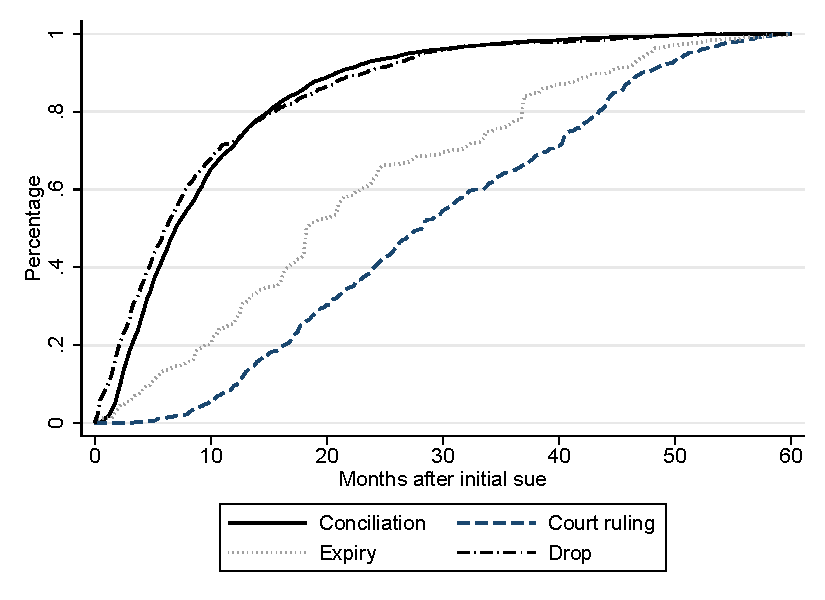
\includegraphics[width=0.7\textwidth]{caseending_overtime.pdf}
        \end{center}
 
 
    \scriptsize
%\begin{figurenotes} 
The figure uses the historical data (5005 casefiles) to plot the cumulative distribution of the duration of the case in months, by type of ending, for the 70 percent of cases concluded by the end of 2015. %Around two-thirds of cases that are settled have a duration of less than one year, and there are very few settlements more than two years after filing. Those ending by court ruling or expiry have much longer average duration.
    %{\scriptsize \textit{Do files: } \texttt{Fig3_caseending_overtime_rep.do}}
% \end{figurenotes}    
\end{figure}

\begin{figure}[!ht]

     \caption{Knowledge about Law and their Own Claims in Lawsuit}
        \label{Knowtheirclaimsfig}
     \begin{center}
        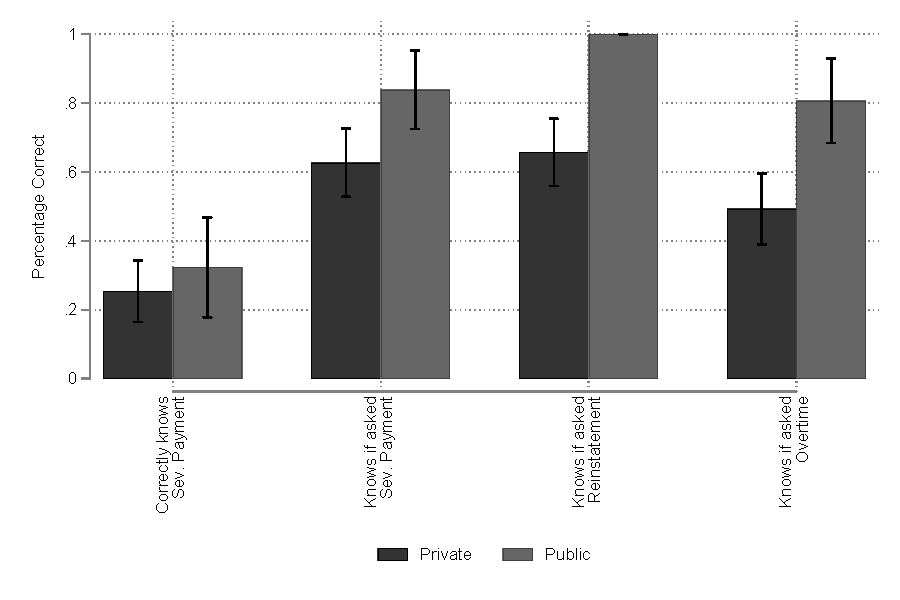
\includegraphics[width=0.7\textwidth]{paper/Figures/knows_all_byType.pdf}
        \end{center}
 
% \begin{figurenotes}
\scriptsize
\textit{Notes:} Data are from baseline survey of Phase 1. The figure shows averages of correct answers for several questions, grouped into: knowledge of the law (panel 1) and knowledge of the content of their own lawsuit (panels 2 to 4). The question for panel (1) is \textit{"In the case of unjustified dismissal, law gives you a constitutional indemnification: Do you know how many days of salary this represents?''}. Panels (2) to (4) correspond to the question: \textit{``Mark the benefits that you claimed in this suit: 1.Constitutional indemnification, 2.Medical insurance, 3.Reinstatement, 4.Overtime, 5.Premium for working Saturdays, 6. Aguinaldo (bonus), 7.Don't know''}. The figure indicates whether the respondent correctly answered items 2, 3 and 4.
        %{\scriptsize \textit{Do files: }  \texttt{knowledge_allbyType}}
% \end{figurenotes}        
\end{figure}

\begin{figure}[!ht]
   
    \caption{Calculator Treatment Format (example) - Phase 1}
       \label{calc_template_p1}
     \begin{center}
        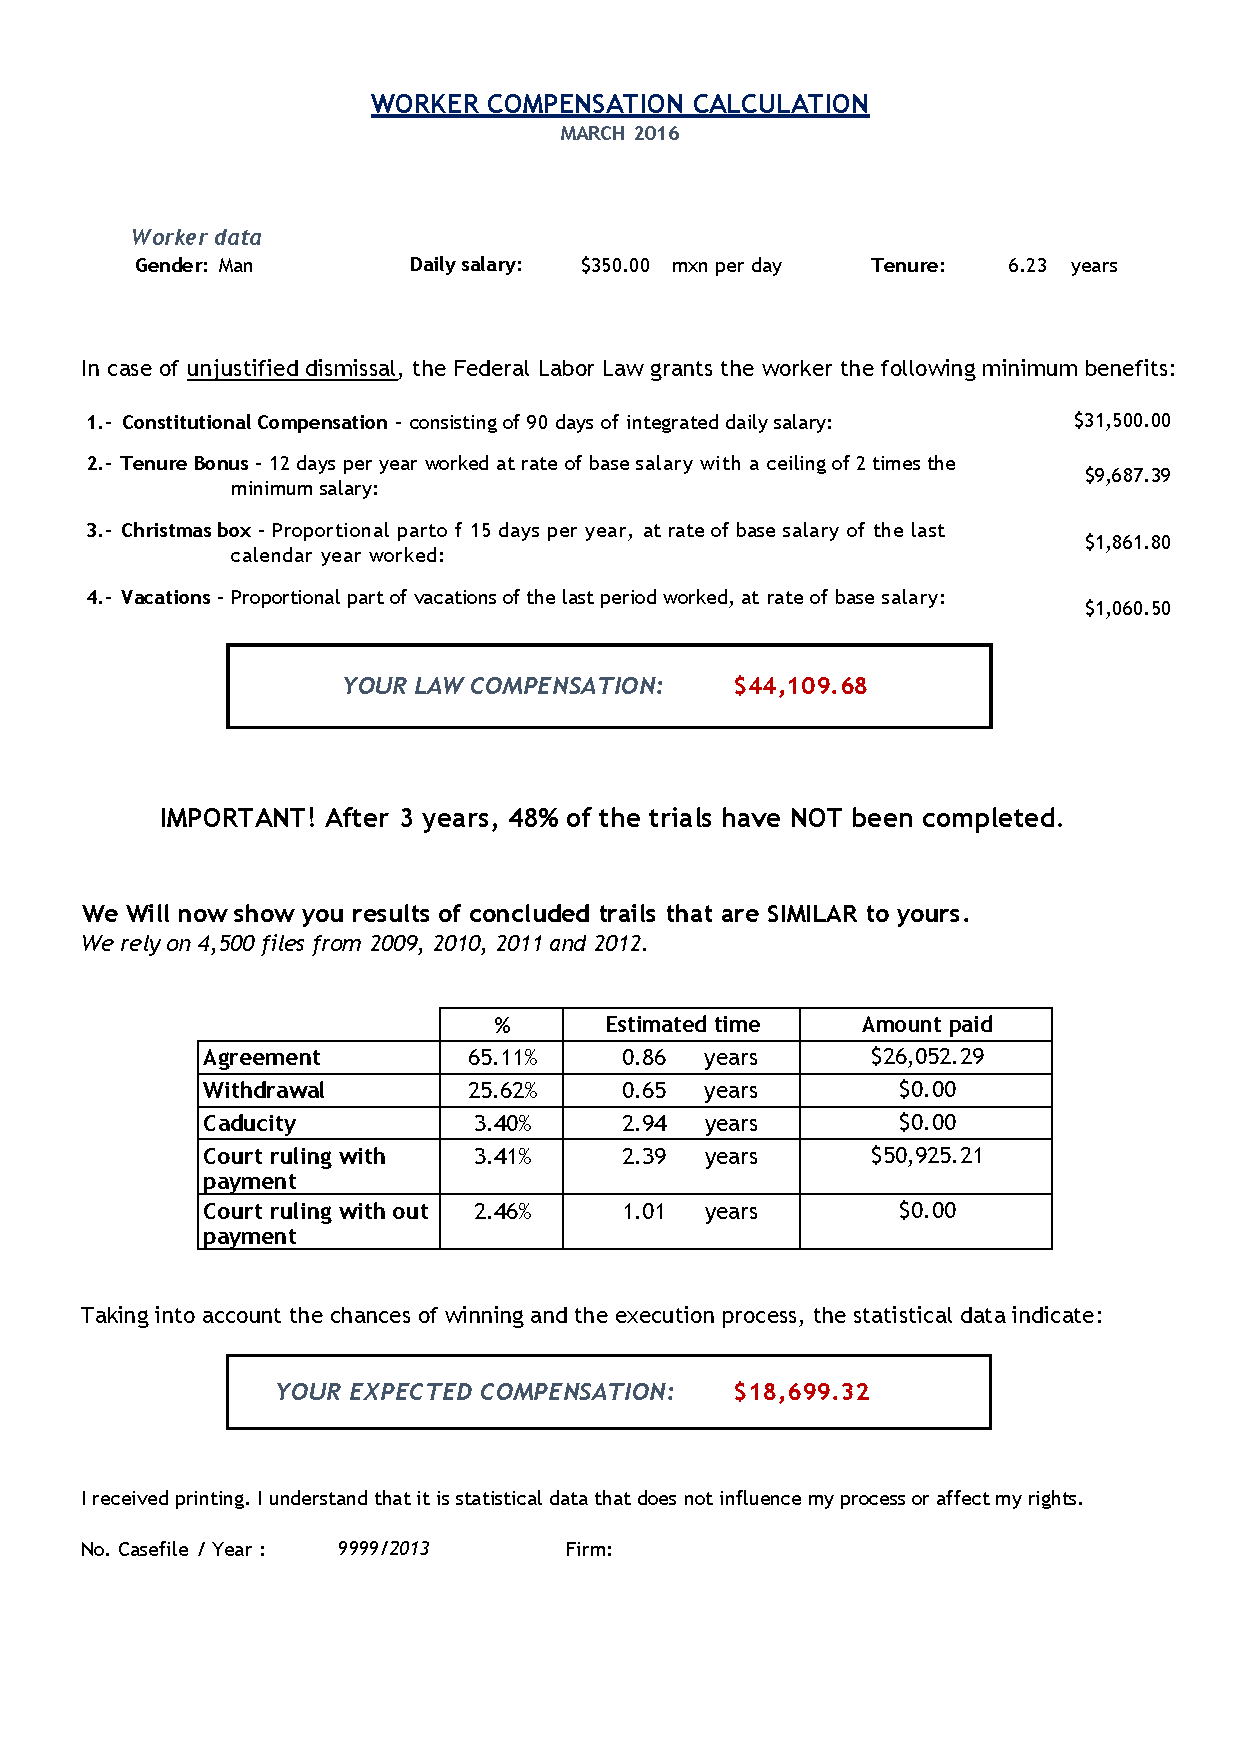
\includegraphics[width=0.75\textwidth]{calctreat_p1.pdf}
        \end{center}
            
 
% \begin{figurenotes}
\scriptsize
\textit{Notes:}The figure shows an example of the calculator use in Phase 1 treatments. The top half described the entitlement by law if the judge rules in favor of the plaintiff, based on data in the case filing. The second half shows what fraction of cases end which way, the average duration and amount for each ending, and the expected value ex-ante saliently in red in the bottom box. The worker and firm name are removed from the example shown here. Parties were told that this information comes from a statistical exercise based on completed historical cases, and that it gives average prediction based on variables of the initial lawsuit described in the calculator treatment.
 %   \end{figurenotes} 
\end{figure}




\begin{figure}[!ht]
    \caption{Calculator predictions}
        \label{calcpredictions}
    \begin{center}
 \begin{subfigure}{0.45\textwidth}
        \caption{PDF}
      \centering
        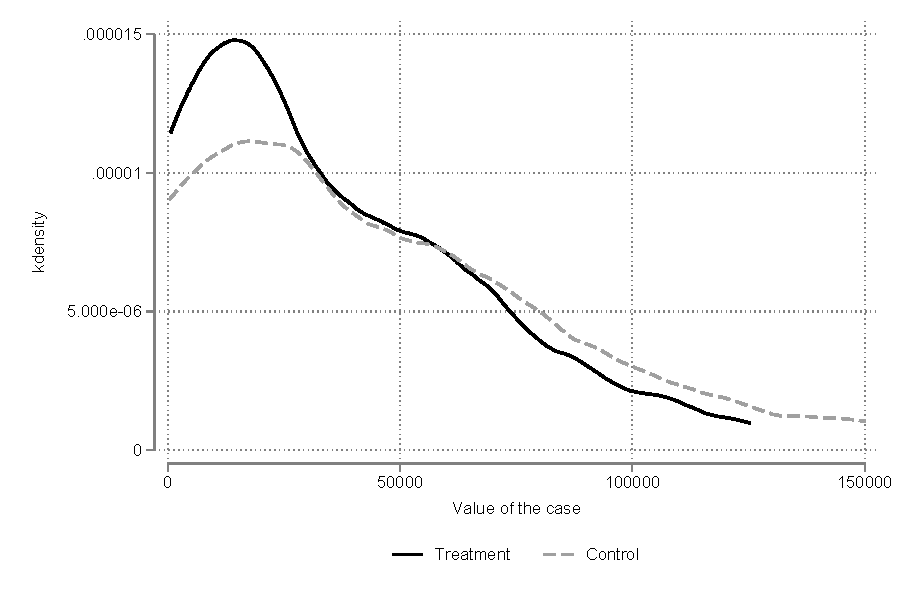
\includegraphics[width=\linewidth]{paper/Figures/pdf_valordecaso.pdf}
    \end{subfigure}
  \begin{subfigure}{0.45\textwidth}
        \caption{CDF}
        \centering
        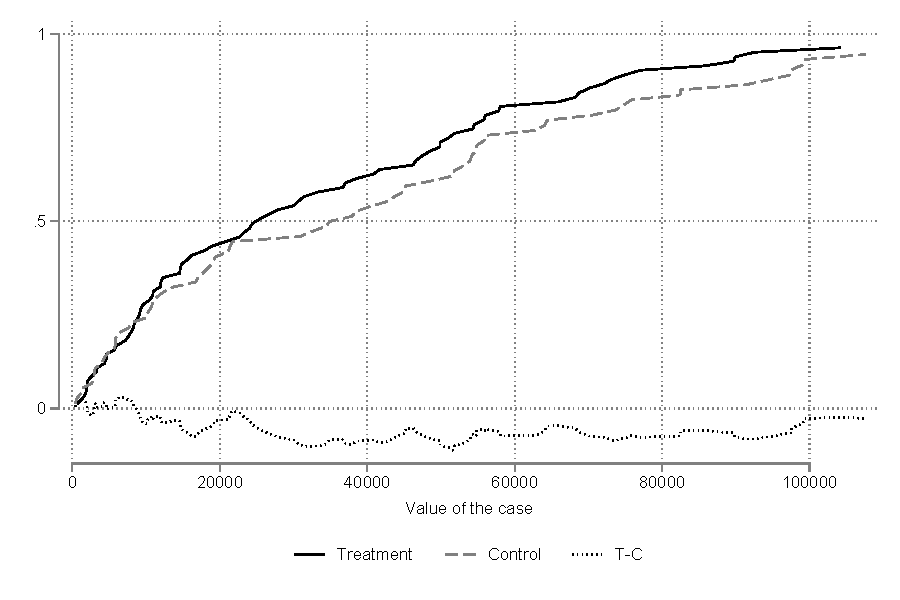
\includegraphics[width=\linewidth]{paper/Figures/cdf_valordecaso.pdf}
    \end{subfigure}
         \end{center}
              \scriptsize
             \textit{Notes: This figure shows the distribution of amounts predicted by the calculator for treatment and control cases ending in settlement. Panel (a) shows the distribution functions, while panel (b) shows the cumulative distribution function. } The dotted line at the bottom shows the net difference in the two distributions at each percentile. The two distributions are not statistically different from one another at conventional levels at any single point or in total.
            %  The dotted line below indicates the points where the difference in the distributions is significant.  Instead of a single global null hypothesis (that the two CDFs are identical), there is a continuum of individual null hypotheses of CDF equality at each point. 
        %\textit{Do file: valordecaso.do} \texttt{}   
\end{figure}

% \begin{figure}[!ht]
%     \caption{Calculator predictions for Settled Cases}
%         \label{CalculatorVSettlements}
%     \begin{center}
%         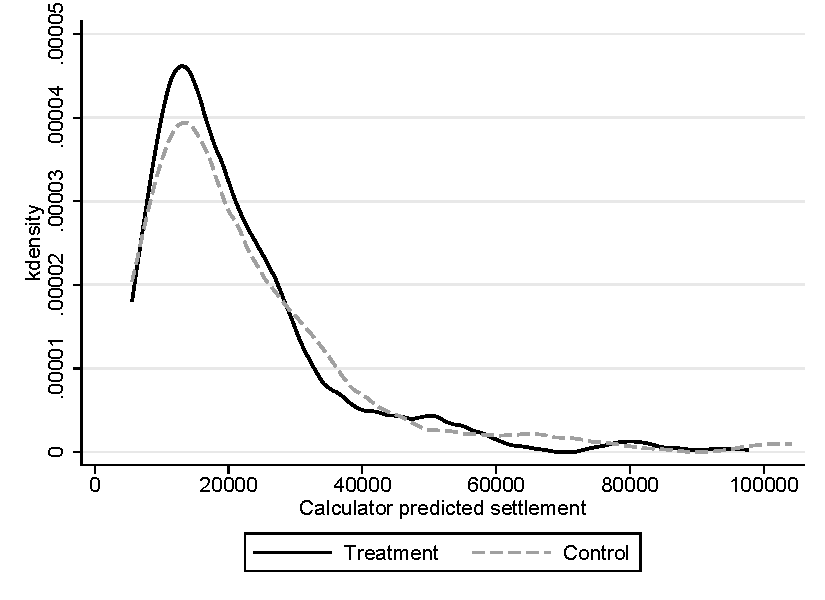
\includegraphics[width=0.6\textwidth]{paper/Figures/CalculatorVSettlements.pdf}
%          \end{center}
%               \scriptsize
%              \textit{Notes: This figure shows the distribution of settlement amounts predicted by the calculator for treatment and control cases ending in settlement. Data are truncated at the 99th percentile to compress the scale.}
%         %\textit{Do file: calculatorDistributionForSettled.do} \texttt{}   
% \end{figure}


\textbf{}

%\begin{figure}[!ht]
%    \caption{Case Duration}
%    \label{Duration_Cases}
%       \begin{center}
%   \begin{subfigure}{0.45\textwidth}
%        \caption{All Case Files}
%       \centering
%        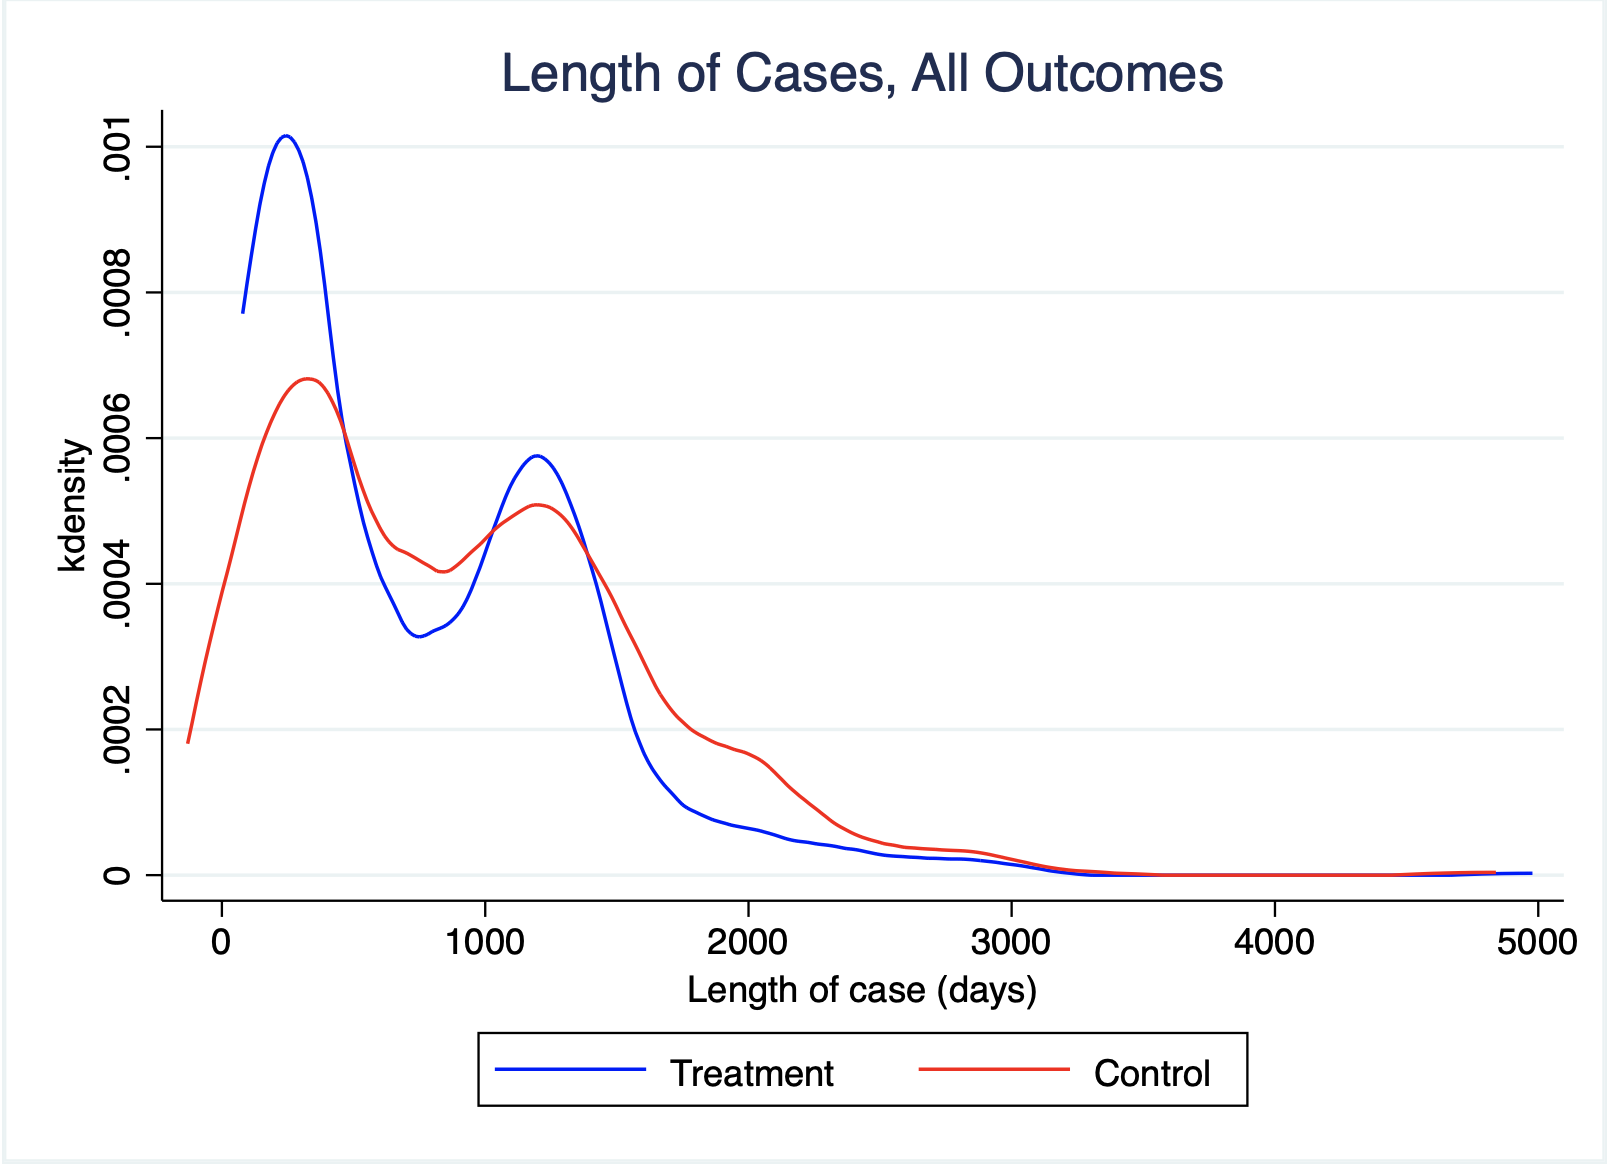
\includegraphics[width=\linewidth]{paper/Figures/Length_All.png}
%    \end{subfigure}
%    \\
%   \begin{subfigure}{0.45\textwidth}
%        \caption{Settlments}
%        \centering
%        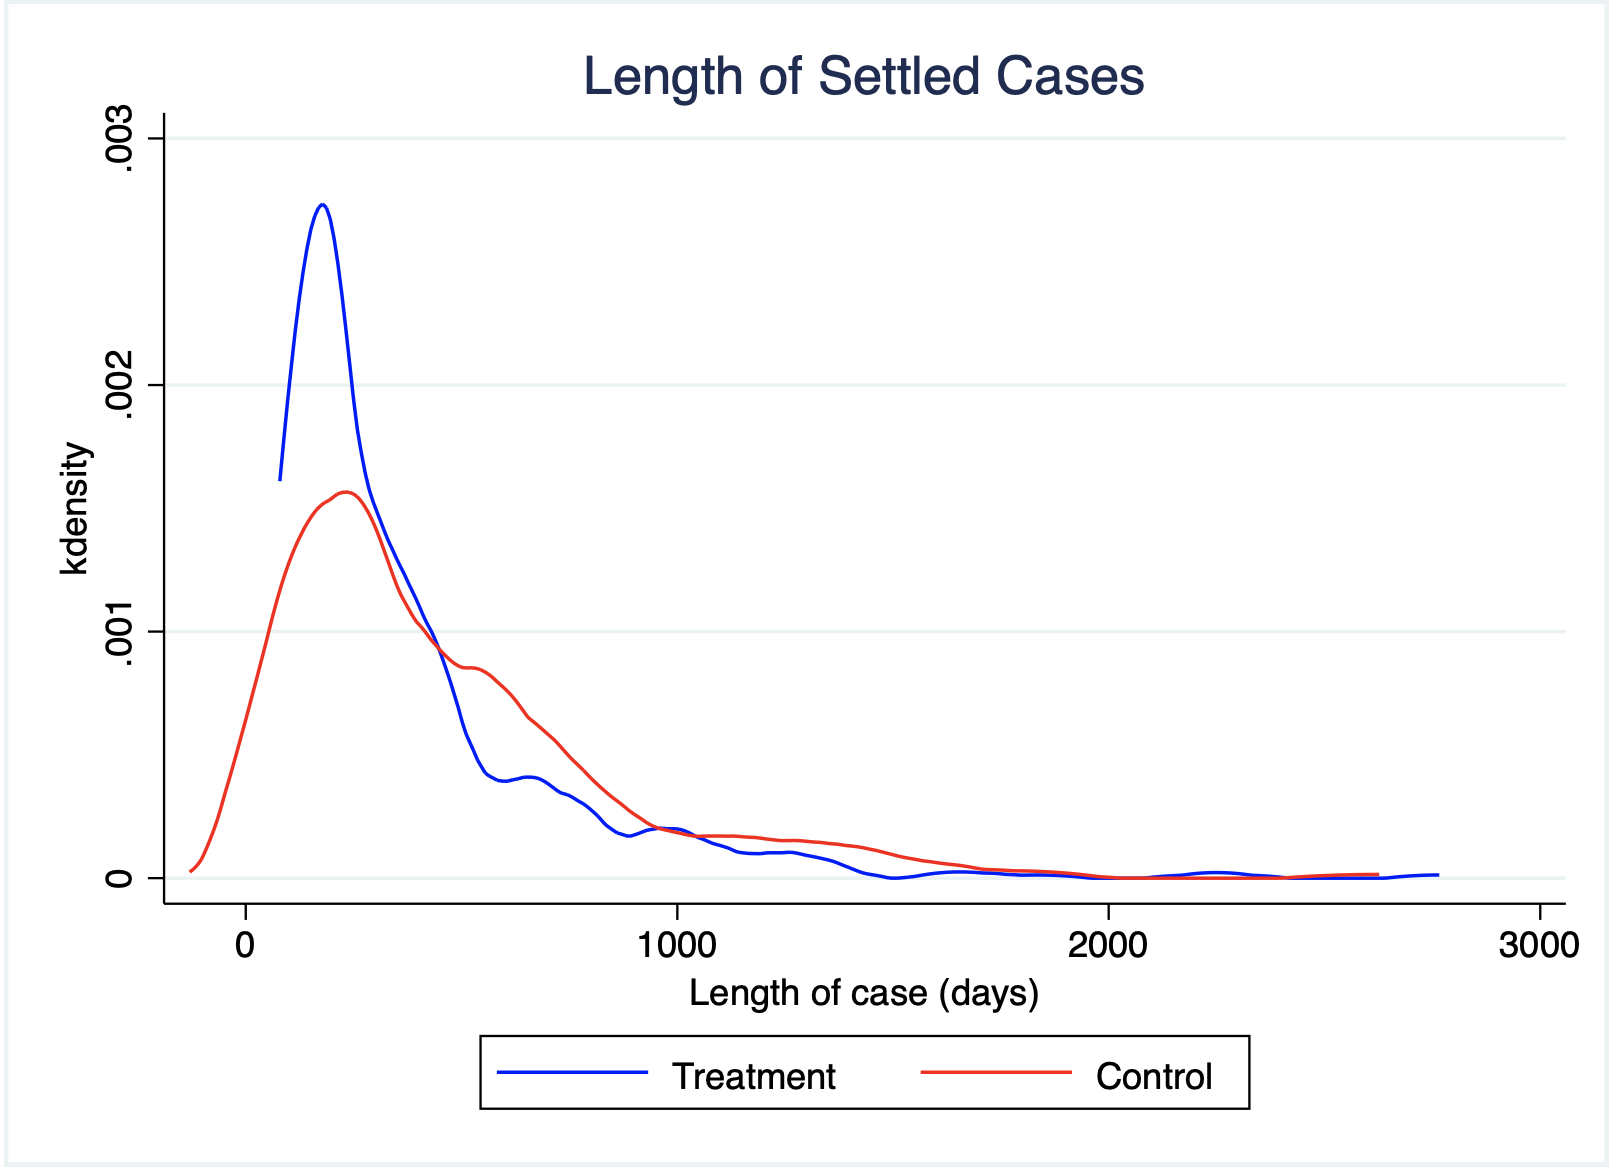
\includegraphics[width=\linewidth]{paper/Figures/Length_Settlements.png}
%    \end{subfigure}
%    \begin{subfigure}{0.45\textwidth}
%           \caption{Judgments}
%        \centering
%        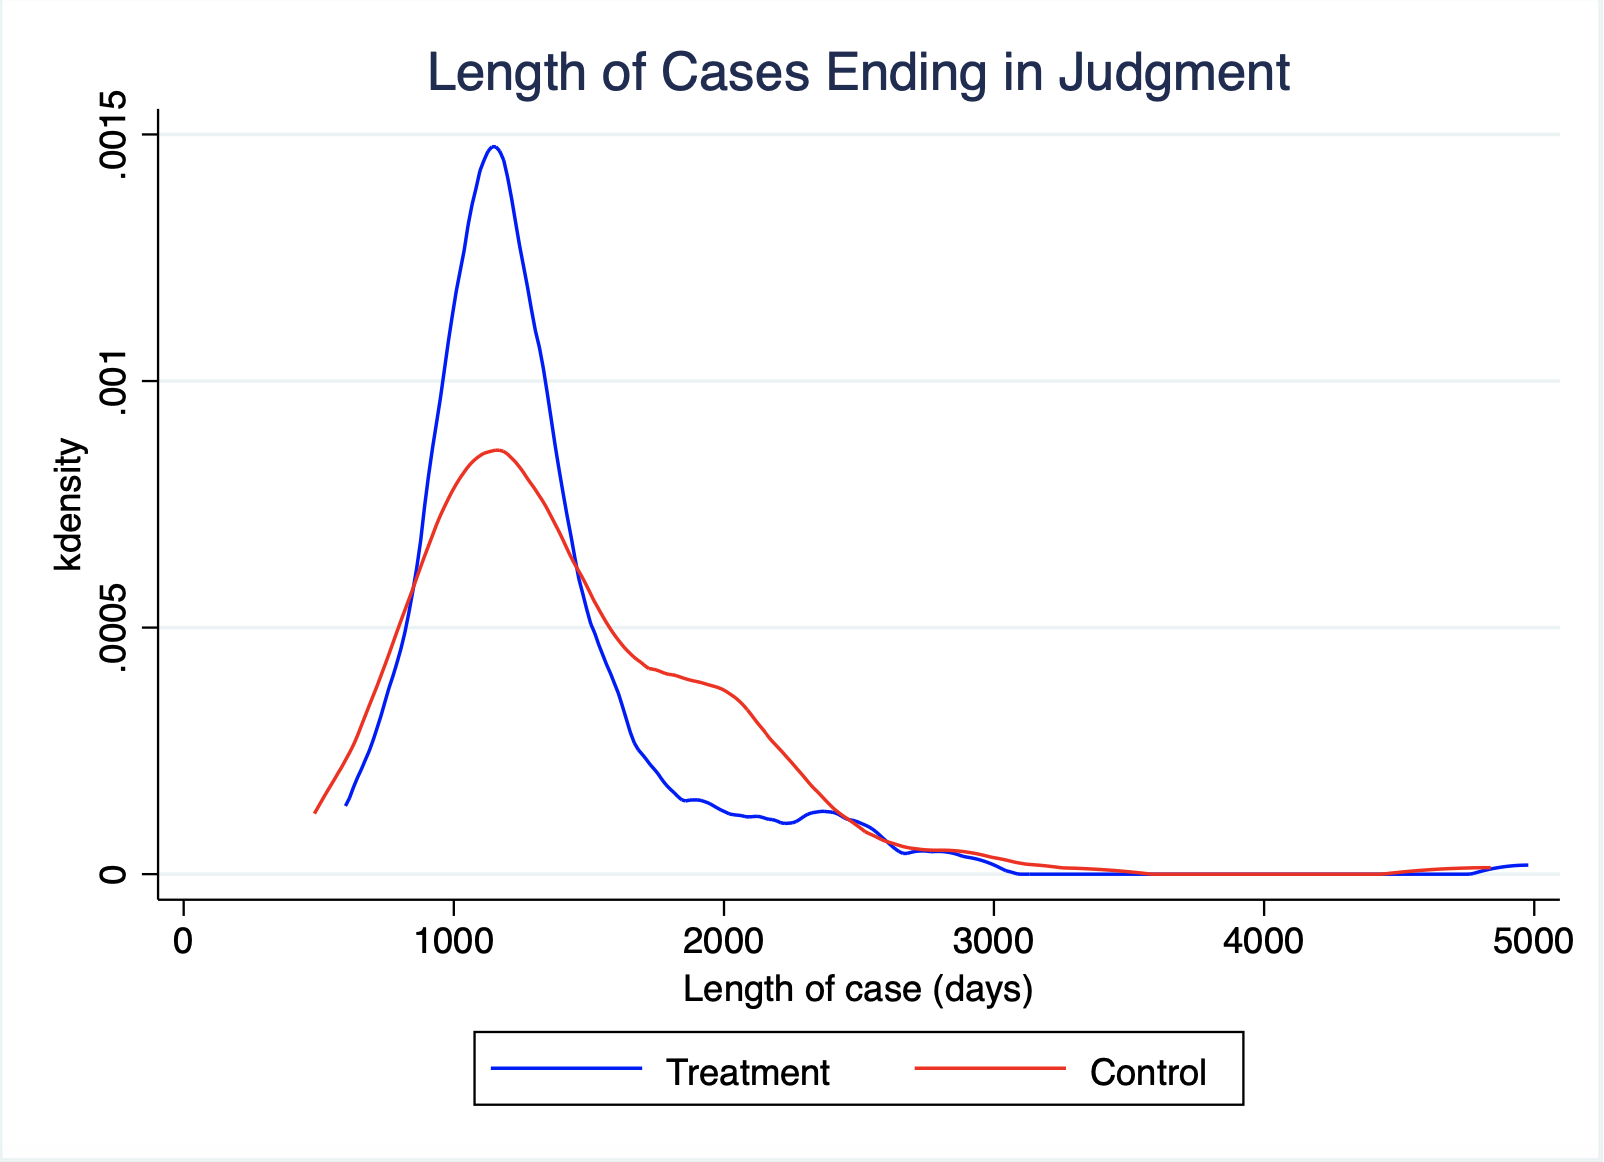
\includegraphics[width=\linewidth]{paper/Figures/Length_Judgments.png}
%        \end{subfigure}
   
%   \end{center}
%      \scriptsize \textit{Notes:} Case length, measured as the number of days from filing to final resolution, for 1,423 cases with any outcome (panel a), 679 cases ending in settlement (panel b) and 333 cases ending in court judgment (panel c). The data are plotted separately for cases assigned to treatment and control. Cases are limited to files with valid filing dates with a private lawyer.
    %   \scriptsize{ \textit{Do file: }  \texttt{oc\_comparison\_B.do}}
%\end{figure}

\begin{figure}[!ht]
    \caption{Unresolved Cases: Calculator Prediction Conditional on Court Win}
        \label{CalculatorCourtWin}
    \begin{center}
        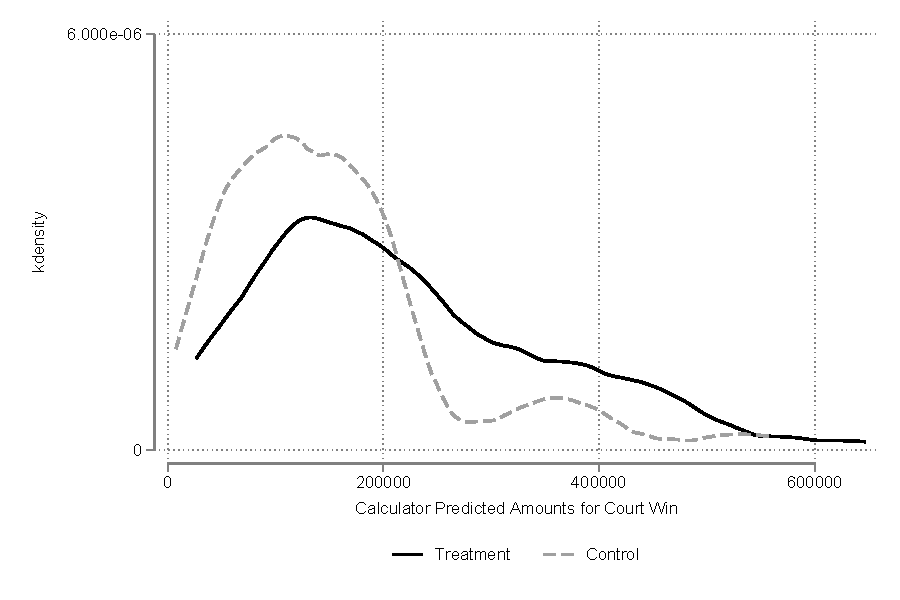
\includegraphics[width=0.6\textwidth]{paper/Figures/Calculator_CourtWin_Unresolved.pdf}
         \end{center}
              \scriptsize
             \textit{Notes:} This figure presents the distribution of recovery amounts predicted by the calculator, conditional on winning a judgment, for treatment and control cases that were unresolved at the time of last data access. Data are truncated at the 99th percentile to compress the scale. Note that the differences between predicted outcomes in treatment and control reflect in part the fact that more of the unresolved cases in the treatment group are from Phase 2, and hence higher-value cases. Figure \ref{Unresolved_Court_ByPhase} in \nameref{appendix_c} shows the distributions by phase. The patterns are similar though somewhat more muted.
        %\textit{Do file: } \texttt{caseValueKdensitiesdo}   
\end{figure}
%\textbf{}

\newpage

\FloatBarrier


\begin{center}
\large{\textbf{Information and Bargaining through Agents: Experimental Evidence from Mexico's Labor Courts}}

%\shortTitle{Information and Bargaining through Agents}

\textit{Joyce Sadka,  Enrique Seira, and Christopher Woodruff}

\Large{\textbf{Online Appendices}}
\end{center}

\section*{Appendix A}
\label{appendix_a}
\title{\Large{\textbf{Mexican Labor Law, Description of Data, and the Calculator}}}
\\

\setcounter{table}{0}
\renewcommand{\thetable}{A.\arabic{table}} 
\setcounter{figure}{0}
\renewcommand{\thefigure}{A.\arabic{figure}} 

The appendix is divided into four sections. The first describes the Mexican labor law and court procedures, the second provides some additional details on the administrative data, the third describes our surveys and response rates, and the fourth describes the calculator we use to make predicted outcomes for the cases in which we intervene. 

\subsection{Mexican Labor Law}

\textbf{Mexican labor Law:} On paper, Mexican labor law is protective of workers. For any employer-initiated separation that is not a '`justified dismissal,'' the law requires severance payment of a minimum of 90 days' wages and benefits. The law provides very few legal bases for a justified dismissal. For example, workers are owed severance if they are fired for low productivity or because of poor market conditions.  As an element of their lawsuit, workers may ask the court to order the firm to rehire them. If they win their case and the firm refuses to rehire them, then they are entitled to an additional severance payment equal to 20 days' wages for each year of tenure at the firm.\footnote{Certain categories of workers (those defined as '`at-will'') are also entitled to to 20 days' wages per year of tenure. An at-will worker is one who is employed in a position of confidence, for example, a driver or a personal security guard. The law recognizes that the employer may need to dismiss the worker if that confidence is broken.} 

\textbf{The Process:} In a firing lawsuit, an initial claim is filed by the worker or her lawyer, and an initial hearing date is set, generally two to three months after the date of filing. The defendant(s) must be notified of the filing and hearing date by a formal court summons that must be delivered in person by an employee of the court. The notification process typically takes 6 months.\footnote{In practice, notification involves substantial corruption, as the lawsuit cannot proceed without it.  \cite{KaplanSadka_notif} shows that when notifiers' work load is assigned randomly and control of case files is taken away from notifiers, rates of successful notification more than double.} Once notification of all defendants has taken place, a '`conciliation, demands, and answers'' hearing takes place. The principal demand in most firing lawsuits is either the base severance pay of 90 days or reinstatement of employment. 

If a settlement cannot be reached then the defendant must answer the lawsuit. Additional hearings are scheduled for presentation and viewing of evidence, after which the written record is closed. All proceedings are conducted by an administrative assistant to the judge. Hearings are transcribed into the case file. The file is passed on to the judge, who writes the final decision. Enforcement of judgments involving payments to the plaintiff is often challenging. A large proportion of firms do not pay the judgment voluntarily, and a seizure of assets must officially be performed by officers of the court. This is  followed by adjudication of liquid assets or sale of non-liquid assets to pay the worker the awarded amount. Given that an interval of six-months between hearings is typical, the fact that there are more than four hearings held in an average case, and the frequent postponement of scheduled hearings due to lack of notification, the average lawsuit continuing to a judge's decision takes over three years. This in spite of the law stipulating that lawsuits should have a maximum duration of 100 days. 

\textbf{Lawyers:} Once a case is filed, lawyers control the lawsuits almost completely. The presence of the parties themselves at the hearings is not compulsory, unless they are to be deposed as part of the evidentiary hearings. By law, workers who are not able to hire a private lawyer must be provided with free public legal assistance from labor lawyers in the public prosecutor's office. Public lawyers are paid a flat wage by the court and may not charge  clients anything further. A public lawyer handles as many as 400 cases concurrently, while administrative data suggest that a normal load for a private lawyer is at most 50 cases. So while public lawyers are generally well qualified, they have an incentive to finish cases quickly in order to reduce their workload. The general perception is that public lawyers do not use creative or aggressive litigation strategies that may have a positive payoff but imply longer cases or more work. 

Private lawyers must be licensed, but obtaining the license is fairly easy and otherwise lawyers are unregulated. Survey data indicate that 82 percent of workers are suing for the first time. Workers have little access to information about where to find a good private lawyer, and often opt for the first one that they run into, with little notion of that lawyer's reputation or previous record. The surveys show that 38 percent of plaintiffs using a private lawyer say that they found the lawyer either just outside the court or in one of the court corridors. Plentiful anecdotal evidence suggests that these '`informal lawyers'' are low-quality and may not serve their clients' best interests. 

Private plaintiff's lawyers typically charge an initial fee of about MXN\$2000 pesos (USD 100) to file the lawsuit and a contingency fee of about 30 percent of any amount collected by the plaintiff. In spite of the contingency fee, their incentives are not perfectly aligned to those of their clients. First, while plaintiffs are party to a single case, the lawyers manage a portfolio of many firing lawsuits with widely differing characteristics, against many different firms. With diversified risk, they may be more willing to take risks on any given case.   Second, filing a low-quality suit is cheap and easy and the lawyers may profit from collecting the filing fee even with no expectation of recovering anything on behalf of the worker.  The plaintiff must ratify settlements of the lawsuit in person, as well as acceptance or rejection of an offer of reinstatement, should the plaintiff's side receive one. Lawyers typically do not bring the plaintiffs to hearings nor do they provide them much detail on the developments in the lawsuit. As will be shown below, the physical presence of the worker at the hearing in which we intervene in the field experiment is crucial for the effectiveness of our intervention. 

 %\footnote{Private lawyers may have incentives to convince a worker to sue and not settle even when it is not in her interest to do so. The most common way of doing this is to inflate the claim by adding elements to it, even if in the end they won't stand up in court (e.g. lost wages, vacation pay, end of year bonus, and overtime), and by exaggerating the worker's salary, which is often paid by the firm totally or partially in an informal way.}
 
 \FloatBarrier
 
\subsection{Administrative Data}

The main source of administrative data are the initial case filings for the historical and experimental cases. For the experimental cases, we also collected data on the phase 1 and 2 case outcomes in December 2018 and in January and July  2020. The historical data are used to develop a predictive model of case outcomes. We then use this model and the data from each experimental case filing to predict outcomes for each case, as described in subsection \ref{calculator_method} below. Because we intervene in many cases at the time of their first hearing, we use only data from the initial case filing. The case files are available in hard copy, and we digitize the variables shown on Table \ref{variable_list}. 

\begin{table}[!ht]
    \caption{Casefile Variable}
    \label{variable_list}
    \begin{center}
        \scriptsize{% Table generated by Excel2LaTeX from sheet 'Variable_list'
\begin{tabular}{p{2.25cm}| p{12cm}}
\toprule
\rowcolor[rgb]{ .267,  .329,  .416} \textcolor[rgb]{ 1,  1,  1}{\textbf{VARIABLE}} & \textcolor[rgb]{ 1,  1,  1}{\textbf{DESCRIPTION}} \\
\midrule
\textbf{Tenure} & Employee's tenure with the employer. \\
\midrule
\textbf{Weekly hours} & Number of hours that the plaintiff worked on a weekly basis. \\
\midrule
\textbf{Reinstatement*} & The plaintiff claims reinstatement. \\
\midrule
\textbf{Severance pay*} & The plaintiff claims constitutional indemnity (three months of integrated salary) that the law dictates for unjustified dismissal. \\
\midrule
\textbf{Lost wages*} & The plaintiff claims lost wages/back pay. \\
\midrule
\textbf{Vacation pay*} & The plaintiff claims accrued vacation days not taken. \\
\midrule
\textbf{Overtime*} & The plaintiff claims overtime pay. \\
\midrule
\textbf{Twenty days compensation*} & The plaintiff claims the payment of compensation (20 days per year worked) that the law dictates for unjustified dismissal for a worker who has the right to be reinstated but the employer refuses to reinstate, or for an at-will employee who cannot ask for reinstatement. \\
\midrule
\textbf{Insurance- IMSSINFOSAR*} & The plaintiff claims the payment of employer contributions that were not made to these institutions, or retroactive registration in the institutions (SAR: retirement savings, IMSS: social security, INFONAVIT: worker's housing fund). \\
\midrule
\textbf{Co-defendant*} & At least one of the codefendants is the IMSS or INFONAVIT or SAR. \\
\midrule
\textbf{Total asked} & The total quantifiable peso amount of the worker's claim. \\
\midrule
\textbf{Minimum legal entitlement} & The quantifiable peso amount of the sum of severance pay, vacation and end of year bonuses of the last year of tenure at the firm. It is a conservative estimate of the minimum amount of money the worker is entitled to if she wins the lawsuit. \\
\bottomrule
\end{tabular}%
}
    \end{center}
     \scriptsize
    \textit{Notes:} 
Detailed description of variables used throughout the paper. Dummy variables are marked with \textbf{*}.
\end{table}


\FloatBarrier

\subsection{Survey Data}

We conducted surveys with participants at the hearings in Phases 1 and 2, and with dismissed workers approaching the court in Phase 3. The surveys in the first two phases had to be very short so that we did not delay the start of hearings. We use one survey instrument for plaintiffs, and another for the lawyers representing both plaintiffs and employers. Table \ref{ss_survey} shows summary statistics for workers and lawyer from phase 1. Table \ref{Table_compliance} shows compliance rates for both the surveys and treatments for the first two phases. We have no measure of noncompliance in phase 3. Every worker who completed the survey and was assigned to treatment received the calculator treatment. However, there were surely dismissed workers who approached the court but did not stop at our information booth. Since the workers approaching the court had no way of know if the given day was assigned to treatment or control, we have no reason to believe there is differential non-compliance across treatment groups on either observable or unobservable characteristics. Hence, non-compliance in phase 3 is an issue of external rather than internal validity.\footnote{Even if every dismissed worker approaching the court had fully complied with the experimental protocol, the sample would not be representative of all aggrieved workers dismissed from Mexico City employers, because many dismissed workers obtain information from public or private lawyers without coming to the court. However, we believe the sample is relevant for understanding the effect of information provision on the decision to file case or settle.}  

\begin{table}[!ht]
     \caption{Survey variables summary statistics}
     \label{ss_survey}
     \begin{center}
     \resizebox{16.5cm}{!}{
     \scriptsize{% Table generated by Excel2LaTeX from sheet 'surveySS'
\begin{tabular}{rrcccc}
\toprule
\multicolumn{6}{c}{\textbf{Panel A: worker characteristics}} \\
\midrule
      &       & Mean  &       &       & Mean \\
      &       & (SD)  &       &       & (SD) \\
      &       & N     &       &       & N \\
\midrule
\multicolumn{2}{l}{Age} & 44.4 & \multicolumn{2}{l}{More than secondary education} & 0.42 \\
\multicolumn{2}{r}{} & (13.2) & \multicolumn{2}{r}{} & (0.50) \\
\multicolumn{2}{r}{} & 102   & \multicolumn{2}{r}{} & 102 \\
\multicolumn{2}{l}{Firm had less than 50 employees} & 0.59  & \multicolumn{2}{l}{Was treated poorly/very poorly by former employer} & 0.55  \\
\multicolumn{2}{r}{} & (0.49) & \multicolumn{2}{r}{} & (0.50) \\
\multicolumn{2}{r}{} & 96    & \multicolumn{2}{r}{} & 102 \\
\multicolumn{2}{l}{Expected probability of winning trial} & 79.0   & \multicolumn{2}{l}{Mean / Median expected recovery (Pesos)} & 97,116 / 21,000 \\
\multicolumn{2}{r}{} & (21.3) & \multicolumn{2}{r}{} & (355,749) \\
\multicolumn{2}{r}{} & 102    & \multicolumn{2}{r}{} & 102 \\
\multicolumn{2}{l}{What would employer report as probability of winning?} & 48.7 & \multicolumn{2}{l}{Expected duration (years)} & 3.64 \\
\multicolumn{2}{r}{} & (34.1) & \multicolumn{2}{r}{} & (9.76) \\
\multicolumn{2}{r}{} & 102   & \multicolumn{2}{r}{} & 102 \\
\multicolumn{2}{l} {Percentage paid to lawyer} & 28.3  & \multicolumn{2}{l} {Has changed lawyer during trial} & 0.09 \\
\multicolumn{2}{r}{} & (11.1) & \multicolumn{2}{r}{} & (0.29) \\
\multicolumn{2}{r}{} & 57   & \multicolumn{2}{r}{} & 102 \\
\multicolumn{2}{r}{} &       & \multicolumn{2}{r}{} &  \\
\midrule
\midrule
\multicolumn{6}{c}{\textbf{Panel B: lawyer characteristics}} \\
\midrule
      &       & \multicolumn{2}{c}{Worker's lawyer} & \multicolumn{2}{c}{Employer's lawyer} \\
\midrule
      &       & \multicolumn{2}{c}{Mean} & \multicolumn{2}{c}{Mean} \\
      &       & \multicolumn{2}{c}{(SD)} & \multicolumn{2}{c}{(SD)} \\
\multicolumn{2}{r}{} & \multicolumn{2}{c}{N} & \multicolumn{2}{c}{N} \\
\midrule
\multicolumn{2}{l}{Age} & \multicolumn{2}{c}{37.8} & \multicolumn{2}{c}{36.6} \\
\multicolumn{2}{r}{} & \multicolumn{2}{c}{(12.4)} & \multicolumn{2}{c}{(11.0)} \\
\multicolumn{2}{r}{} & \multicolumn{2}{c}{231} & \multicolumn{2}{c}{223} \\
\multicolumn{2}{l}{Tenure} & \multicolumn{2}{c}{9.25} & \multicolumn{2}{c}{18.7} \\
\multicolumn{2}{r}{} & \multicolumn{2}{c}{(8.88)} & \multicolumn{2}{c}{(143.3)} \\
\multicolumn{2}{r}{} & \multicolumn{2}{c}{181} & \multicolumn{2}{c}{193} \\
\multicolumn{2}{l}{More than 100 historical cases} & \multicolumn{2}{c}{0.49} & \multicolumn{2}{c}{0.61} \\
\multicolumn{2}{r}{} & \multicolumn{2}{c}{(0.50)} & \multicolumn{2}{c}{(0.49)} \\
\multicolumn{2}{r}{} & \multicolumn{2}{c}{231} & \multicolumn{2}{c}{223} \\
\multicolumn{2}{l}{More than 30 current lawsuits} & \multicolumn{2}{c}{0.60} & \multicolumn{2}{c}{0.68} \\
\multicolumn{2}{r}{} & \multicolumn{2}{c}{(0.49)} & \multicolumn{2}{c}{(0.47)} \\
\multicolumn{2}{r}{} & \multicolumn{2}{c}{231} & \multicolumn{2}{c}{223} \\
\multicolumn{2}{l}{Less than 50 employees} & \multicolumn{2}{c}{0.65} & \multicolumn{2}{c}{0.46} \\
\multicolumn{2}{r}{} & \multicolumn{2}{c}{(0.48)} & \multicolumn{2}{c}{(0.50)} \\
\multicolumn{2}{r}{} & \multicolumn{2}{c}{173} & \multicolumn{2}{c}{151} \\
\multicolumn{2}{l}{Percentage paid to lawyer} & \multicolumn{2}{c}{29.7} & \multicolumn{2}{c}{} \\
\multicolumn{2}{r}{} & \multicolumn{2}{c}{(7.79)} & \multicolumn{2}{c}{} \\
\multicolumn{2}{r}{} & \multicolumn{2}{c}{172} & \multicolumn{2}{c}{} \\
\multicolumn{2}{l}{Expected probability of winning trial} & \multicolumn{2}{c}{72.2} & \multicolumn{2}{c}{70.5} \\
\multicolumn{2}{r}{} & \multicolumn{2}{c}{(20.1)} & \multicolumn{2}{c}{(21.5)} \\
\multicolumn{2}{r}{} & \multicolumn{2}{c}{231} & \multicolumn{2}{c}{223} \\
\multicolumn{2}{l}{Mean / Median expected recovery (Pesos)} & \multicolumn{2}{c}{237,958 / 35,000} & \multicolumn{2}{c}{66,885 / 11,000} \\
\multicolumn{2}{r}{} & \multicolumn{2}{c}{(1,482,120)} & \multicolumn{2}{c}{(285,657)} \\
\multicolumn{2}{r}{} & \multicolumn{2}{c}{231} & \multicolumn{2}{c}{223} \\
\multicolumn{2}{l}{Expected duration (years)} & \multicolumn{2}{c}{3.94} & \multicolumn{2}{c}{4.17} \\
\multicolumn{2}{r}{} & \multicolumn{2}{c}{(2.30)} & \multicolumn{2}{c}{(2.54)} \\
\multicolumn{2}{r}{} & \multicolumn{2}{c}{231} & \multicolumn{2}{c}{223} \\
\bottomrule
\bottomrule
\end{tabular}%
}
     }
     \end{center}
     \scriptsize
     \textit{Notes:} Summary statistics of survey variables for Pilot 1 participants. The parties were surveyed before the case. The plaintiff was surveyed if present and the plaintiff's lawyer was surveyed otherwise. The firm was almost never present, so the lawyer was surveyed from the defendant's side. The number of responses varies across questions due to item non-responses. 
 \end{table}
 % Do file: surveyP1SS.do

\begin{landscape}
\begin{table}[!ht]
    \caption{Compliance Rate}
    \label{Table_compliance}
    \begin{subtable}{1\textwidth}
      \centering
        \caption{Phase 1}
        \scriptsize{% Table generated by Excel2LaTeX from sheet 'Compliance'
\begin{tabular}{lrcccccccccccc}
\toprule
\multicolumn{1}{c}{Group} & \multicolumn{1}{c}{N} & \multicolumn{4}{c}{Compliance with treatment} & \multicolumn{4}{c}{Compliance with baseline survey} & \multicolumn{4}{c}{Compliance with exit survey} \\
\midrule
\midrule
      &       & Plaintiff & Defendant & Both  & Any   & Plaintiff & Defendant & Both  & Any   & Plaintiff & Defendant & Both  & Any \\
\midrule
Control & 321   & -     & -     & -     & -     & 50.78 & 35.51 & 8.72  & 77.57 & 39.88 & 24.3  & 5.61  & 58.57 \\
Calculator & 315   & 77.65 & 73.03 & 75.81 & 79.72 & 48.25 & 33.65 & 12.38 & 69.52 & 38.63 & 25.86 & 9.66  & 54.83 \\
\bottomrule
\end{tabular}%
}
    \end{subtable}%
    
    \bigskip
    \begin{subtable}{1\textwidth}
      \centering
        \caption{Phase 2}
        \scriptsize{% Table generated by Excel2LaTeX from sheet 'complianceP2'
\begin{tabular}{lrrrrrrrrr}
\toprule
Group & \multicolumn{1}{l}{N} & \multicolumn{4}{c}{Compliance with treatment} & \multicolumn{4}{c}{Compliance with survey} \\
\midrule
\midrule
      &       & \multicolumn{1}{l}{Plaintiff} & \multicolumn{1}{l}{Defendant} & \multicolumn{1}{l}{Both} & \multicolumn{1}{l}{Any} & \multicolumn{1}{l}{Plaintiff} & \multicolumn{1}{l}{Defendant } & \multicolumn{1}{l}{Both } & \multicolumn{1}{l}{Any} \\
\midrule
\midrule
Control & 329   & \multicolumn{1}{l}{-} & \multicolumn{1}{l}{-} & \multicolumn{1}{l}{-} &       & \multicolumn{1}{l}{-} & \multicolumn{1}{l}{-} & \multicolumn{1}{l}{-} & \multicolumn{1}{l}{-} \\
Calculator & 762   & 72.7  & 63.78 & 49.08 & 87.4  & 54.33 & 48.29 & 49.08 & 87.4 \\
\bottomrule
\end{tabular}%
}
    \end{subtable}
    
      \bigskip
    \begin{subtable}{1\textwidth}
      \centering
        \caption{\% Shows up}
        \scriptsize{% Table generated by Excel2LaTeX from sheet 'show_up'
\begin{tabular}{lcccc}
\toprule
      & \multicolumn{2}{c}{Phase 1} & \multicolumn{2}{c}{Phase 2} \\
\midrule
\midrule
      & Control & Calculator & Control & Calculator \\
\midrule
\midrule
\multicolumn{1}{p{4.055em}}{Employee } & 0.193 & 0.197 & 0.122 & 0.165 \\
Emp Lawyer & 0.847 & 0.832 & 0.85  & 0.853 \\
Firm Lawyer & 0.738 & 0.762 & 0.434 & 0.444 \\
\bottomrule
\bottomrule
\end{tabular}%
}
    \end{subtable}
            \scriptsize
           \\
           \\
           \\
  \textit{Notes:} 
  Compliance rate for each phase, both for treatment and survey. Each panel shows the percentage compliance with treatment and survey for plaintiff' side, defendant's side, both, and any. In phase 1, we did not measure compliance with treatment at the party level but rather at the casefile level, so that for example the 74.16 under the column "both" for compliance with treatment means that among the casefiles for which both parties showed up to the hearing, we were able to give the calculator to at least one of the parties in 74.16 percent of the cases. Also, in phase 1 we had an exit survey in addition to the baseline survey. In phase 2, we did measure compliance with the treatment by party. On the other hand, note from panel (b) that since in phase 2 control days were days that no implementing personnel were present in the subcourts, we have neither treatment nor survey compliance for the control group. Panel (c) shows from the court's administrative data who shows up to the hearings for each of the two phases, split by employee, employee lawyer, and firm lawyer.
    % \textit{Scripts: } \texttt{complianceTable.do, ComplianceP2Tables.do, showUp.do}
\end{table}
\end{landscape}







\begin{table}[!ht]
  \caption{Balance table}
    \label{balance_table}
    \begin{center}
    \scriptsize{% Table generated by Excel2LaTeX from sheet 'Balance'
\begin{tabular}{lccccccccc}
\toprule
      & \multicolumn{3}{c}{Phase 1} & \multicolumn{3}{c}{Phase 2} & \multicolumn{2}{c}{Phase 1/2} &  \\
\midrule
\midrule
      & C     & T     & p-value & C     & T     & p-value & C     & T     & p-value \\
\midrule
\midrule
At will worker & 0.12  & 0.1   & 0.64  & 0.1   & 0.07  & 0.2   & 0.11  & 0.08  & 0.09* \\
Tenure at firm & 4.85  & 4.56  & 0.58  & 4.97  & 4.11  & 0.07* & 4.91  & 4.22  & 0.04** \\
Public Lawyer & 0.1   & 0.12  & 0.56  & 0.06  & 0.06  & 0.76  & 0.08  & 0.08  & 0.84 \\
\% Severance pay & 0.82  & 0.85  & 0.31  & 0.81  & 0.79  & 0.54  & 0.82  & 0.81  & 0.75 \\
Daily wage & 875.16 & 624.24 & 0.03** & 617.35 & 600.52 & 0.85  & 740.05 & 606.57 & 0.06* \\
\% Tenure bonus & 0.79  & 0.85  & 0.06* & 0.8   & 0.78  & 0.55  & 0.8   & 0.8   & 0.85 \\
Entitlement & 97526.49 & 71391.91 & 0.03** & 63189.71 & 68890.8 & 0.5   & 78992.76 & 69519.73 & 0.18 \\
Presence employee & 0.19  & 0.2   & 0.91  & 0.16  & 0.19  & 0.13  & 0.17  & 0.19  & 0.3 \\
Presence emp law & 0.85  & 0.83  & 0.59  & 0.92  & 0.89  & 0.14  & 0.88  & 0.87  & 0.52 \\
Presence firm & 0.03  & 0.02  & 0.23  & 0.01  & 0.02  & 0.22  & 0.02  & 0.02  & 0.8 \\
Presence firm law & 0.74  & 0.76  & 0.49  & 0.79  & 0.78  & 0.83  & 0.76  & 0.78  & 0.53 \\
\midrule
\midrule
Observations & 321   & 315   & 0.58  & 328   & 768   & 0.2   & 649   & 1083  & 0.11 \\
\bottomrule
\end{tabular}%
}
    \end{center}
     \scriptsize
    \textit{Notes:} 
    Balance table on basic and strategic variables. The first three columns show phase 1, with means for each variable in the control, and calculator treatment groups toether with a p-value for the null of equality. The next three columns show the control and treatment for phase 2, and finally the last three columns combine both phases. *, **, and *** indicates a difference that is significant at the 10\%, 5\%, and 1\% level, respectively, as compared with the control group.\\
    
     To identify outliers for these variables, we follow \cite{BILLOR2000279}, and use STATA's command \texttt{bacon}. Using this methodology we identified 5 outliers, and as luck would have it, all 5 are in the control group (and all in phase 1). Removing these 5 observations is enough to achieve balance. Main results do not change when removing this 5 observations.
     
    % \textit{Do file: } \texttt{balance_corrected.do}
\end{table}


\subsection{The Calculator}
\label{calculator_method}

As described in the paper, one of the treatment arms required giving workers information about predicted outcomes for their case. In this subsection we describe the variables and machine-learning models we use to develop these predictions. Since the objective of the project was to provide the parties with the most accurate predictions possible, we considered several different models for each outcome of interest. The models were estimated using 70 percent of the data and then tested on the remaining 30 percent. We based the predictions on the model that yielded the lowest error in the test sample. Among the models we considered are the most common machine learning models, since these have shown in other settings to be very flexible and improve prediction accuracy.

We want to predict a series of outcomes, some of which are continuous and some of which are discrete. Different models are appropriate for these two types of outcomes, so we organize our discussion by first describing the discrete outcomes of interest and the models tested for those outcomes, and then describe the continuous outcomes of interest and the models we tested for those outcomes. We then describe the calculator templates used in both the first and second phase of the project. 

 For the calculators used in both phases, and for both the continuous and discrete models, we fed the models with the same set of input variables, all from the initial case filing. This is because, for operational reasons we could not use procedures that occur after the filing of the lawsuit, such as evidence submission. Also, the court wanted us to develop a parsimonious calculator that could be used in pre-judicial conciliation meetings prior to the plaintiff filing suit.


\subsubsection*{Discrete outcome models}

The expected payment made to the plaintiff is a function of which party prevails and the amount transferred conditional on the outcome. There are five ways a case can end:


\begin{enumerate}
    \item \textbf{Settlement:} The case may end with a voluntary agreement between the parties where the  the plaintiff accepts a sum of money to cease the lawsuit and renounce the legal right to sue again for the same reason. To be valid, these settlements must be registered at the court, and therefore included in our administrative data.  
    
    \item \textbf{Court ruling with positive compensation:} Cases may proceed to a ruling by a judge that decides which side is wins the lawsuit and how much should be paid to the plaintiff. We classify an outcome as Court ruling with positive compensation if the case ends in a ruling by the judge and the worker actually collects a positive amount.\footnote{Because court rulings with positive collection are uncommon (3.3 percent of cases) we face the the problem of unbalancedness of our court rulings sample. To deal with this problem we used a Synthetic Minority Over-Sampling Technique (see \href{http://jair.org/media/953/live-953-2037-jair.pdf}{Chawla et.al., 2002}) and did a 80-20 train vs.~test split on our data.}
    
    \item \textbf{Court ruling with zero compensation:}
    The judge may also rule in the defendant's favor. In that event the worker receives nothing. However, the worker may also receive nothing if the judge rules in her favor, but she is unable to recover any of the judgment amount from the defendant. Defendants use a variety of strategies to avoid paying judgments, so the “win but collect nothing” outcome is not uncommon. The court records that we digitized did not allow us to differentiate between these two outcomes. We do not see this as an important shortcoming since from the point of view of the plaintiff what matters is the amount she receives.
   
    \item \textbf{Dropped:} A case can be dropped by the plaintiff at any time during the legal proceedings. The difference between dropped and settlement is that it can be done unilaterally by the plaintiff and no payment to the defendant is registered. Our understanding is that when cases are dropped it is because the plaintiff has little evidence to support the case. It is a decision of the plaintiff and not a mandate by the court.
    
    \item \textbf{Expiry:} Finally, a labor suit may expire if the court requires information to continue the procedure, including items of evidence presented by one of the parties that the court needs to view before concluding the hearings procedure if proofs are not provided in a span of 4 months.

\end{enumerate}

In our historical data of cases filed in 2011 and completed by the end of 2015, 63.3 percent end in settlement, 2.0 percent in a court ruling with positive collection, 6.6 percent with a court ruling with nothing collected, 20.3 percent expire and 7.6 percent are dropped.


We want to estimate the probability that a case with characteristics $X_i$ ends in each of the five ways described above. We have a choice of estimating a single multinomial model or separate bivariate outcome models. We chose the bivariate option for simplicity. But to ensure that the  probabilities summed to one, we set the probability of expiry equal one minus the sum of the probabilities of the other four outcomes.\footnote{We also estimated a multinomial model. The results were similar, which is why we chose the bivariate models for simplicity.} We therefore estimated models for four bivariate outcomes, using each the following methods: (a) Logistic Regression, (b) Probit, (c) Random Forest\footnote{We performed grid search in order to find the best hyperparameter setting. We compared 7 different models with the number of trees ranging between 900 and 1500. Our final model resulted in a Random Forest of 1200 CARTs, which yielded an 86 percent accuracy rate on test classification.}, (d) Single-hidden-layer Neural Network (20 nodes in the hidden layer and 10\% weight decay), (e) Gradient Boosting.\footnote{This was implemented with off the shelf models in R : e1071, randomForest, neuralnet, caTools, mboost.}  Models were estimated in a random sample training set made of 70 percent of the observation. The remaining 30 percent was used as a test set. For each model hyperparameters were chosen to minimize mean square error in the test set (MSE-T) using cross-validation. Once hyperparameters for each model were chosen, we chose among those optimized models bases on their mean square error. For each of the 5 discrete outcomes we want to predict we kept the model with the highest correlation between Y and $\hat{Y}$ in the test set.\footnote{For the outcome of settlement, we find that the correlation between Y and $\hat{Y}$ is very slightly higher for Random Forest than for Logit, but we use the Logit model because it was simpler to implement in the field.} Table \ref{ml_models_comparison_disc} shows the accuracy rate for each of these 5 outcomes and for each of the 5 models, highlighting in grey the one chosen. The correlations range from 0.61 to 0.93 for the models selected. 





 \begin{table}[H]
     \caption{Fit assessment of discrete calculator models}
     \label{ml_models_comparison_disc}
 \begin{subtable}{0.85\textwidth}
     \caption*{Phase 1: Discrete outcomes}
     \raggedleft
     \scriptsize{\begin{tabular}{lcccccc}
\toprule
                     & N    & Logit & Probit & Random Forest & Neural Network & Gradient Boosting \\
\midrule
\midrule
Settlement           & 2075 & \cellcolor[rgb]{ .929,  .929,  .929} 0.61  & 0.61   & 0.62        & 0.57           & 0.40              \\
Losing court ruling  & 2075 & 0.67  & 0.69   & \cellcolor[rgb]{ .929,  .929,  .929} 0.74          & 0.65           & 0.62              \\
Winning court ruling & 2075 & 0.67  & 0.69   & \cellcolor[rgb]{ .929,  .929,  .929} 0.75         & 0.70           & 0.67              \\
Expiry               & 2075 & \cellcolor[rgb]{ .929,  .929,  .929} 0.93  & 0.93   & 0.93          & 0.93           & 0.93              \\
Drop                 & 2075 & \cellcolor[rgb]{ .929,  .929,  .929} 0.78  & 0.78   & 0.78          & 0.74           & 0.78             \\
\bottomrule
\end{tabular}}
 \end{subtable}%
   
     \bigskip
 \begin{subtable}{1\textwidth}
       \centering
         \caption*{Phases 2 and 3: Discrete outcomes}
         \scriptsize{\begin{tabular}{lcccccc}
\toprule
                     & N    & Logit & Probit & Random Forest & Neural Network & Gradient Boosting \\
\midrule
\midrule
Accuracy           & 432 &  0.71  & 0.72   & \cellcolor[rgb]{ .929,  .929,  .929} 0.89  & 0.80   & 0.75 \\
\bottomrule
\end{tabular}}
 \end{subtable}
 \\
 \\
 \\
 \scriptsize
   \textit{Notes:} Some statistics on the predictive power of the models considered for both -Phase 1 and Phase 2- calculator calibration processes. Statistics for models chosen for each problem are shown in bold. We show $Corr(y, \hat{y})$ for continuous outcomes. We considered random forests both for continuous and categorical outcome variables, using the algorithm's regression and classification methods, respectively.
%     \textit{RScripts: } \texttt{calc\_predictions.R}
 \end{table}

To assess which variables are the most correlated we find the elasticity between each of the covariates and the predictions of the models selected for each of the outcomes. 

\begin{figure}[H]
    \caption{Variable importance for discrete models}
    \label{PredictorsDiscrete1}
    \begin{center}
    \begin{subfigure}{0.475\textwidth}
        \caption{Settlement}
        \centering
        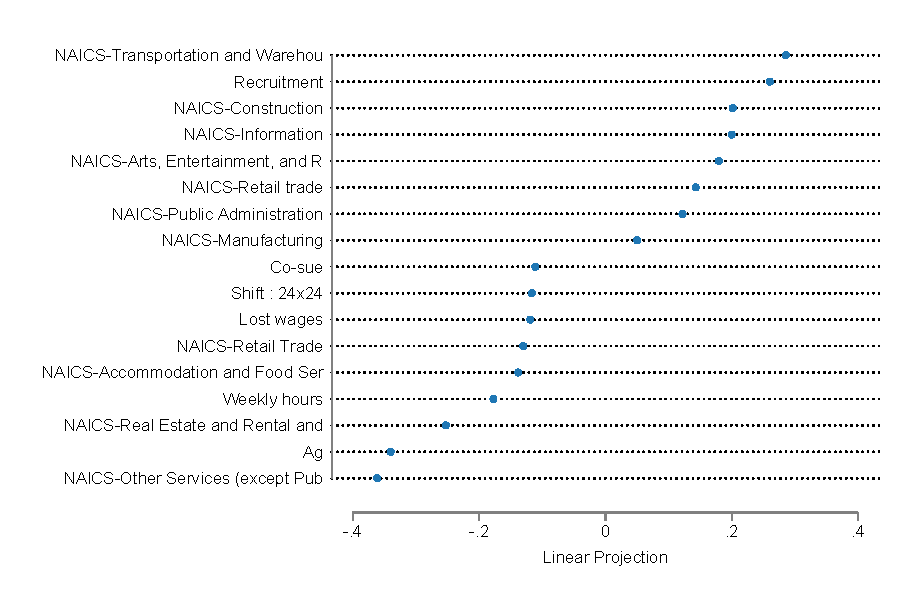
\includegraphics[width=\textwidth]{paper/Figures/coef1_m1.pdf}
    \end{subfigure}
    \begin{subfigure}{0.475\textwidth}
        \caption{Losing court ruling}
        \centering
        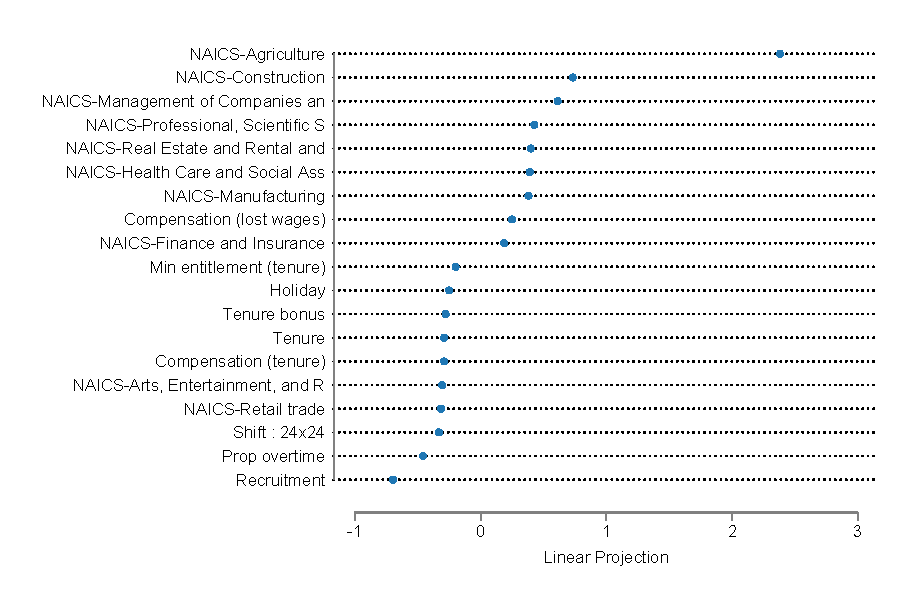
\includegraphics[width=\textwidth]{paper/Figures/coef1_m2.pdf}
    \end{subfigure}
    \begin{subfigure}{0.475\textwidth}
        \caption{Winning court ruling}
        \centering
        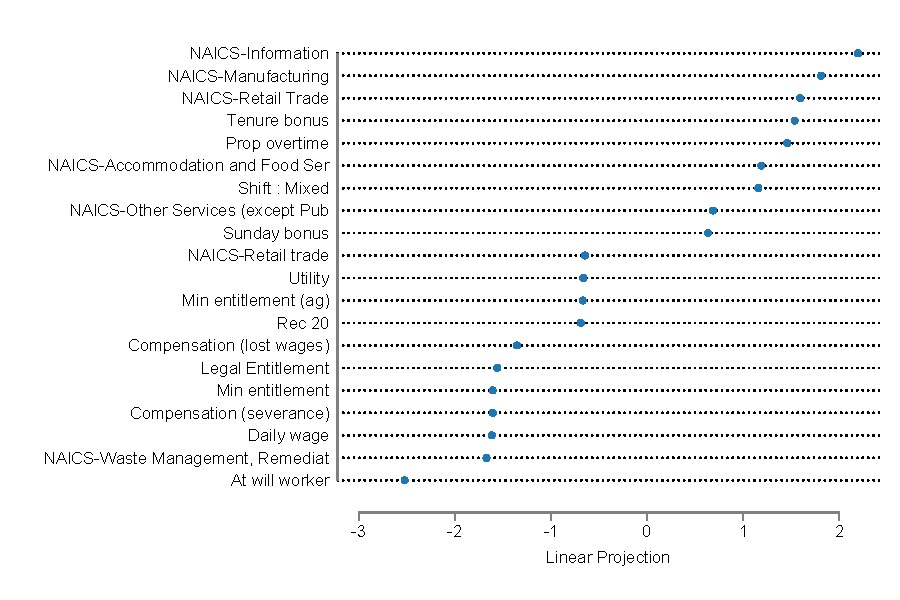
\includegraphics[width=\textwidth]{paper/Figures/coef1_m3.pdf}
    \end{subfigure}
    \begin{subfigure}{0.475\textwidth}
        \caption{Drop}
        \centering
        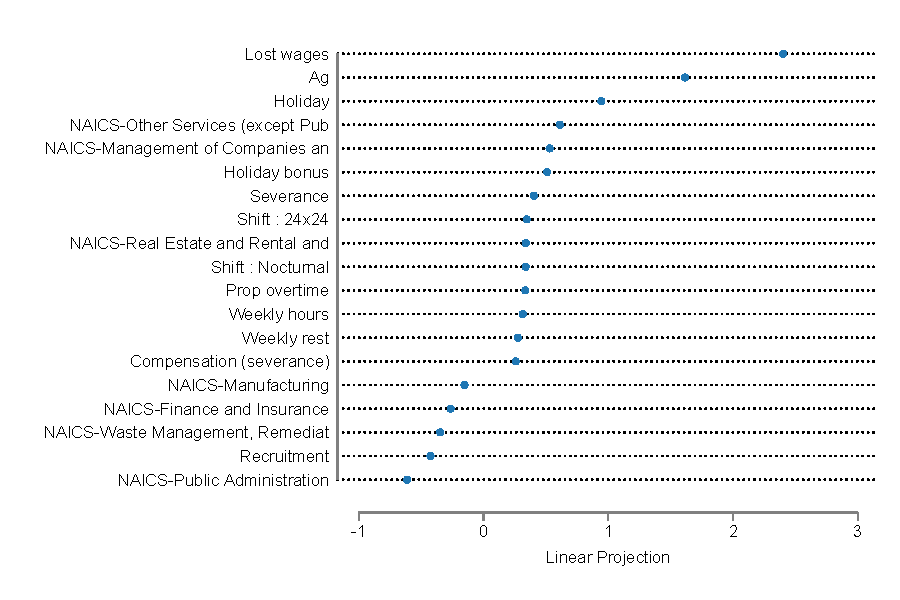
\includegraphics[width=\textwidth]{paper/Figures/coef1_m4.pdf}
    \end{subfigure}  
    \begin{subfigure}{0.475\textwidth}
        \caption{Winning on court ruling (Phase 2 \& 3)}
        \centering
        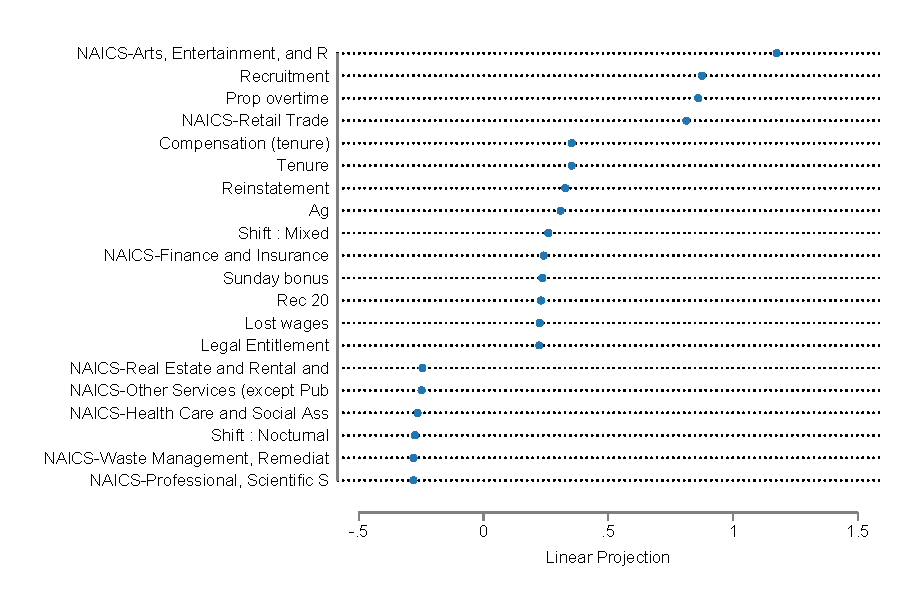
\includegraphics[width=\textwidth]{paper/Figures/coef1_m5.pdf}
    \end{subfigure}      
    \end{center}
     \scriptsize   This figure shows the main features and the role they play in each of the above models. We estimate the effect of this features on the predictions made by this models : $\log{\widehat{pr_i}} = \alpha + \beta_j \log{X_{i,j}} + \epsilon$. Note that we are leaving out all but the variable in question. Qualitatively, these betas can be used to assess the elasticity of the prediction function with the features, they can be interpreted as the elasticity of the partial effect of variable $X_{j}$ on the model's prediction. We only plot the 20 (out of 72) most important features defined as the ones with the biggest estimates in absolute value.   
          %\footnotesize{ \textit{Do file: }  \texttt{coefplots.do}}
\end{figure}






\subsection*{Continuous outcome variables}
Several relevant outcomes are continuous variables. We focus on three continuous variables to be provided to the parties: 

\begin{enumerate}
\item \textit{Amount collected conditional on a positive payment:} This is the peso amount actually collected by the plaintiff in the each of the two outcomes where they payments are positive: settlement and judgment in favor of the plaintiff, with recovery. The other endings all result in zero payments. 
\item \textit{Probability of Positive Recovery:} From the historical data for each casefile we know if the worker in fact was paid a positive amount or not (i.e. won the case in the court ruling and could indeed collect, or settled and got a positive amount).
\item \textit{Duration of the case:} The number of months from the filing of the case to the date when it ended. As a significant share of the cases were not resolved by the end of 2015, we discuss censoring below.
\end{enumerate}

For the continuous outcomes, we estimated a set of four different models for each of the two prediction problems.\footnote{Considering both regular and logarithmic models that would be eight different models for each outcome. The logarithmic models help to tackle the skewness of our dependent variable.} The four models were: (a) OLS regression, (b) GLM Boosting, (c) Random Forest\footnote{We perfomed grid search in order to find the best hyperparameter setting. We compared 7 different models with the number of trees ranging between 900 and 1500. Our final model resulted in a Random Forest of 1200 CARTs, which yielded an 86\% accuracy rate on test classification.}, (d) Ridge Regression\footnote{This was done with the libraries in R: e1071, randomForest, neuralnet, caTools, mboost.} \footnote{We also run the OLS and Random Forest models using logged data. In phase 2, we changed the models we estimated to include Kernel regression, running both OLS and Kernel in levels and logs. We do not present here the Boosted, Random Forest and Ridge regressions. The $corr(\hat{y^{j}},\hat{y^{k}})$ between the predicted values of model $j$ and model $k$ for the union of all models is above 0.8 for all models.}. As with the discrete variables, for each model the hyperparameters were chosen to minimize mean square error in the test set (MSE-T) using cross-validation. Once hyperparameters for each model were chosen, we chose among those optimized models based on their Mean Absolute Percentage Deviation (MAPD). 

Finally we also wanted to predict the duration of the trial from initial suit to termination. We used the data with models similar to those described for the amount collected. However, for phase 2 the predictions from these models were very noisy: the models could not beat a simple average within each type of ending, so we decided to present the simple average within each type of termination rather than a model as a function of observables. 

As with the discrete outcomes, Table \ref{ml_models_comparison_cont} shows the accuracy rate for settlement and duration outcomes and for each of the six models, highlighting in grey the ones chosen. The correlations range from 0.61 to 0.76 for the models selected for total compensation, but from 0.08 to 0.93 for the five duration outcomes. 
\\


\begin{landscape}
\begin{center}
  \begin{table}[H]
     \caption{Fit assessment of continuous calculator models}
     \label{ml_models_comparison_cont}
 \begin{subtable}{0.85\textwidth}
     \caption*{Phase 1: Continuous outcomes}
     \raggedleft
     \scriptsize{\begin{tabular}{lccccccc}
\toprule
 Ending type & N & Regression & Log-regression & Boosted regression & Random Forest & Log-Random Forest & Ridge Regression \\ 
\midrule
\midrule
\multicolumn{8}{c}{Total Compensation} \\ 
\midrule
Settlement  & 1236 & 0.61 & 0.55  & 0.61 & 0.63 & \cellcolor[rgb]{ .929,  .929,  .929} 0.61 & 0.61  \\
Court Ruling   & 66   & 0.70 & \cellcolor[rgb]{ .929,  .929,  .929} 0.76  & 0.70 & 0.49 & 0.28  & 0.67  \\ 
\midrule
\multicolumn{8}{c}{Duration} \\ 
\midrule
Settlement  & 1236 & 0.07 & 0.07  & \cellcolor[rgb]{ .929,  .929,  .929} 0.08 & 0.05 & 0.07   & 0.07  \\
Losing court ruling  & 49   & \cellcolor[rgb]{ .929,  .929,  .929} 0.93 & 0.94  & 0.93 & 0.87 & 0.81   & 0.93  \\
Winning court ruling & 66   & 0.64 & 0.65  & 0.64 & 0.47 & 0.44   & \cellcolor[rgb]{ .929,  .929,  .929} 0.65  \\
Expiry & 118  & 0.35 & 0.34  & \cellcolor[rgb]{ .929,  .929,  .929} 0.37 & 0.29 & 0.39   & 0.42  \\
Drop   & 468  & 0.20 & 0.16  & 0.19 & 0.13 & \cellcolor[rgb]{ .929,  .929,  .929} 0.17   & 0.05 \\
\bottomrule 
\end{tabular}
}
 \end{subtable}%
   
     \bigskip
 \begin{subtable}{1\textwidth}
       \centering
         \caption*{Phases 2 and 3: Continuous outcomes}
         \scriptsize{\begin{tabular}{lccccc}
\toprule
  Ending type  & N & Regression & Kernel regression & Log-regression & Log-kernel regression \\
\midrule
\midrule
\multicolumn{6}{c}{Total Compensation} \\ 
\midrule
Settlement   & 3130 & 0.59    & 0.46     &  \cellcolor[rgb]{ .929,  .929,  .929} 0.69     & 0.63     \\
Court ruling & 105  & \cellcolor[rgb]{ .929,  .929,  .929} 0.44    & 0.30     & 0.18     & -0.06   \\
\bottomrule
\end{tabular}}
 \end{subtable}
 
  \scriptsize
   \textit{Notes:} Some statistics on the predictive power of the models considered for both -Phase 1 and Phase 2- calculator calibration processes. Statistics for models chosen for each problem are shown in bold. We show $Corr(y, \hat{y})$ for continuous outcomes. We considered random forests both for continuous and categorical outcome variables, using the algorithm's regression and classification methods, respectively.
%     \textit{RScripts: } \texttt{calc\_predictions.R}
 \end{table}
 \end{center}
\end{landscape}


\begin{figure}[H]
    \caption{Variable importance for continuous models (total compensation)}
    \label{}
    \begin{center}
    \begin{subfigure}{0.475\textwidth}
        \caption{Settlement}
        \centering
        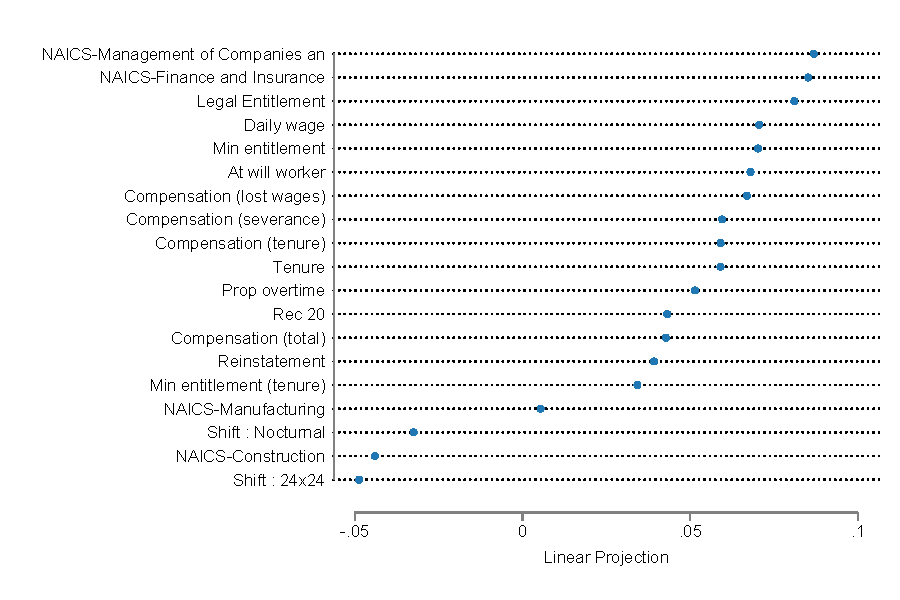
\includegraphics[width=\textwidth]{paper/Figures/coef1_m6.pdf}
    \end{subfigure}
    \begin{subfigure}{0.475\textwidth}
        \caption{Court ruling}
        \centering
        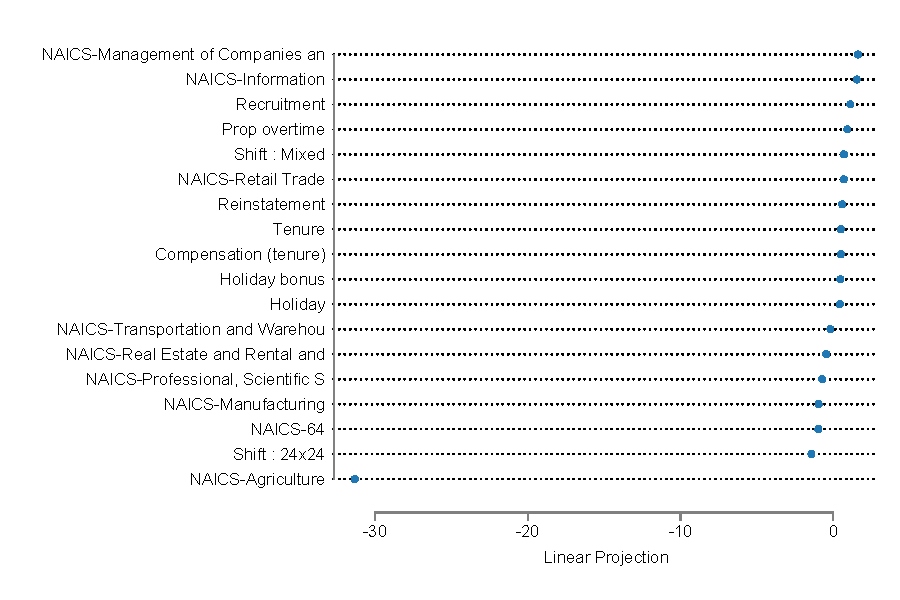
\includegraphics[width=\textwidth]{paper/Figures/coef1_m7.pdf}
    \end{subfigure}
   \begin{subfigure}{0.475\textwidth}
        \caption{Settlement (Phase 2 \& 3)}
        \centering
        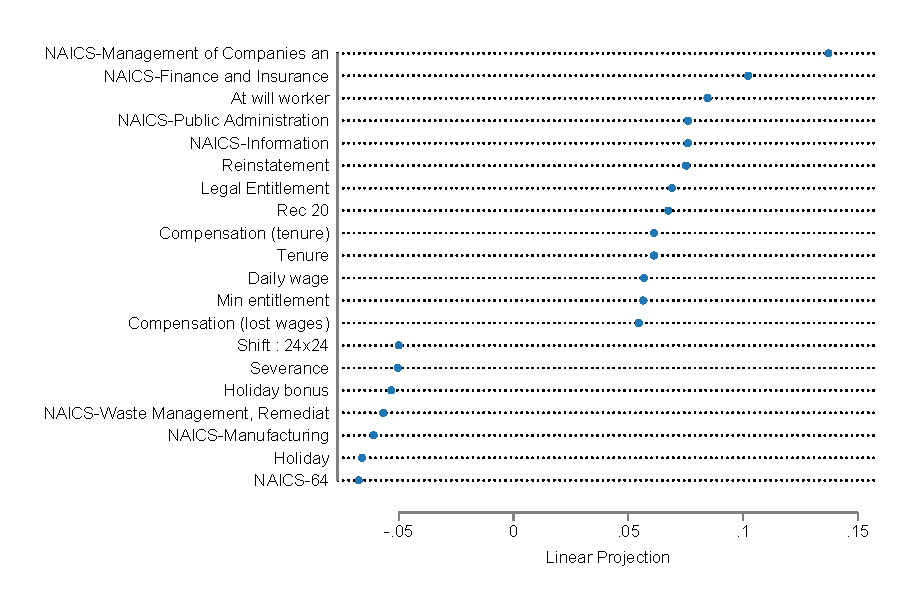
\includegraphics[width=\textwidth]{paper/Figures/coef1_m8.pdf}
    \end{subfigure}
    \begin{subfigure}{0.475\textwidth}
        \caption{Court ruling (Phase 2 \& 3)}
        \centering
        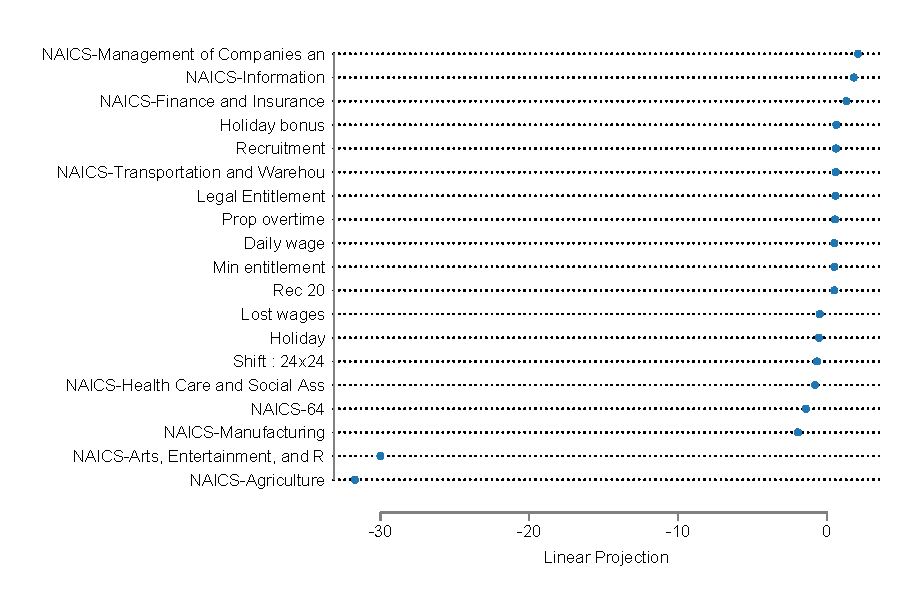
\includegraphics[width=\textwidth]{paper/Figures/coef1_m9.pdf}
    \end{subfigure}     
    \end{center}
     \scriptsize   This figure shows the main features and the role they play in each of the above models. We estimate the effect of this features on the predictions made by this models : $\log{\widehat{pr_i}} = \alpha + \beta_j \log{X_{i,j}} + \epsilon$. Note that we are leaving out all but the variable in question. Qualitatively, these betas can be used to assess the elasticity of the prediction function with the features, they can be interpreted as the elasticity of the partial effect of variable $X_{j}$ on the model's prediction.
     We only plot the 20 (out of 72) most important features defined as the ones which exhibit the higher correlation in absolute value. 
          %\footnotesize{ \textit{Do file: }  \texttt{coefplots.do}}
\end{figure}




\begin{figure}[H]
    \caption{Variable importance for continuous models (duration)}
    \label{PredictorsCont2}
    \begin{center}
    \begin{subfigure}{0.475\textwidth}
        \caption{Settlement}
        \centering
        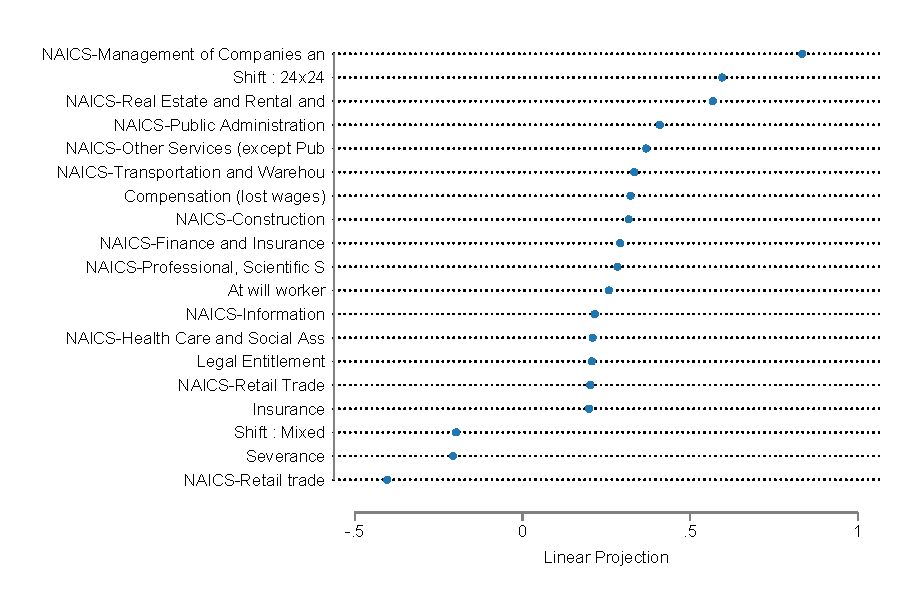
\includegraphics[width=\textwidth]{paper/Figures/coef1_m10.pdf}
    \end{subfigure}
    \begin{subfigure}{0.475\textwidth}
        \caption{Losing court ruling}
        \centering
        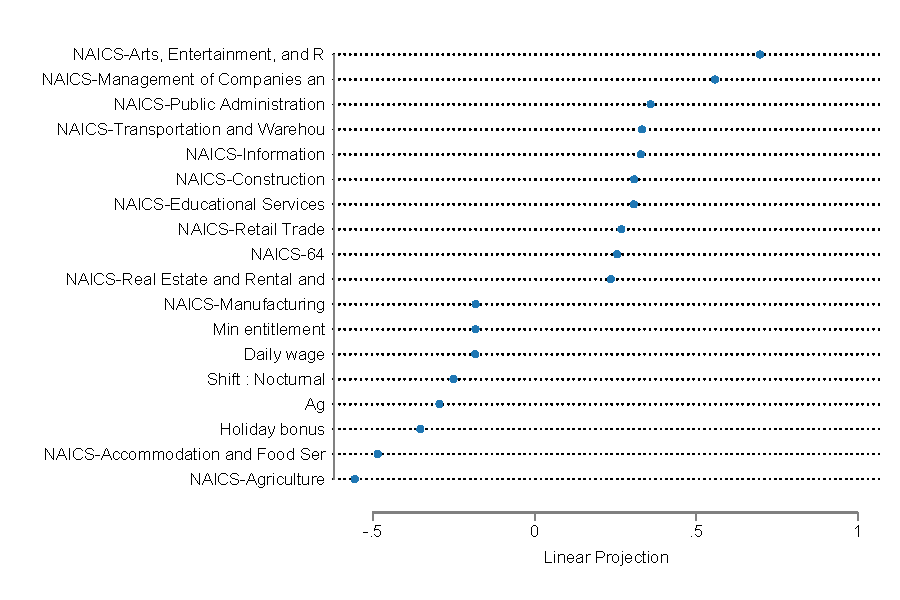
\includegraphics[width=\textwidth]{paper/Figures/coef1_m11.pdf}
    \end{subfigure}
   \begin{subfigure}{0.475\textwidth}
        \caption{Winning court ruling}
        \centering
        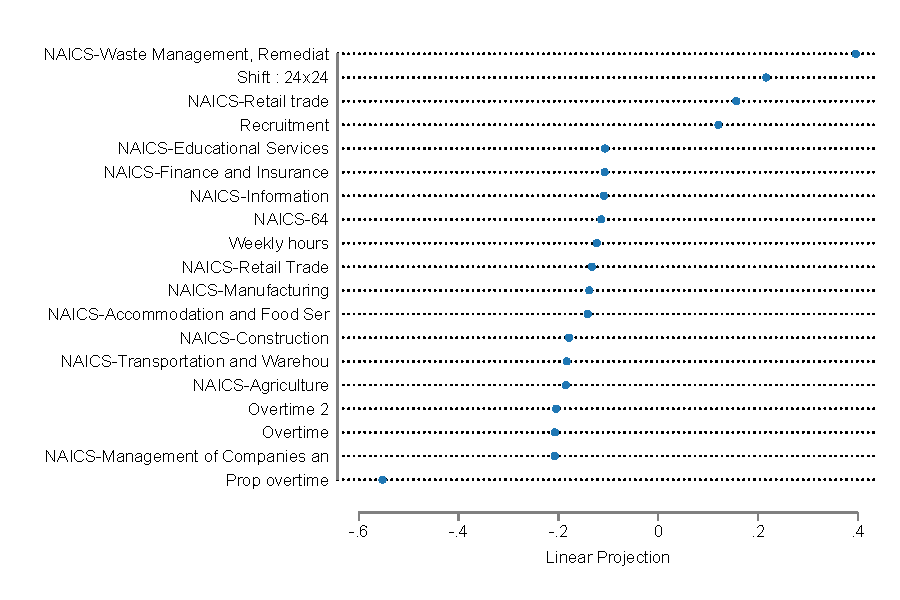
\includegraphics[width=\textwidth]{paper/Figures/coef1_m12.pdf}
    \end{subfigure}
    \begin{subfigure}{0.475\textwidth}
        \caption{Expiry }
        \centering
        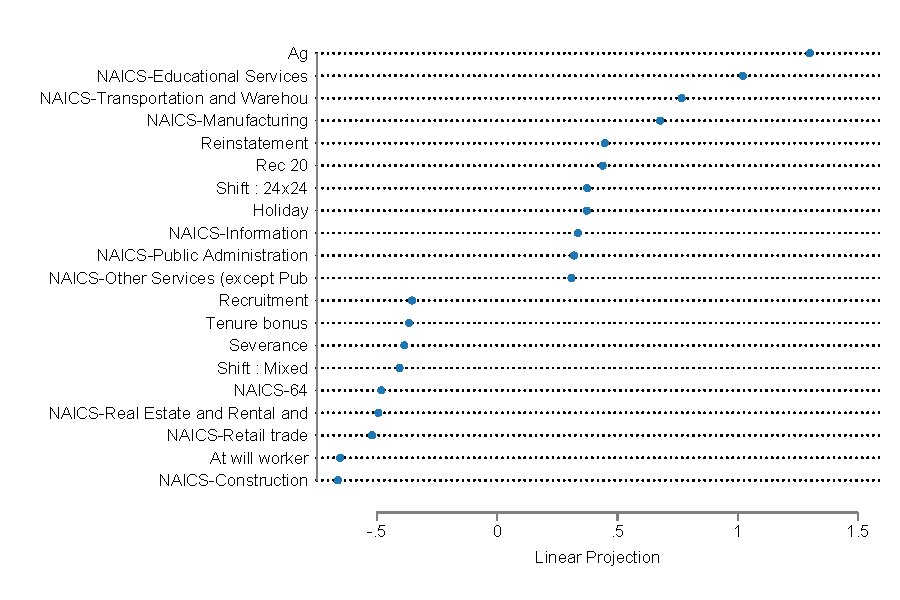
\includegraphics[width=\textwidth]{paper/Figures/coef1_m13.pdf}
    \end{subfigure}     
        \begin{subfigure}{0.475\textwidth}
        \caption{Drop }
        \centering
        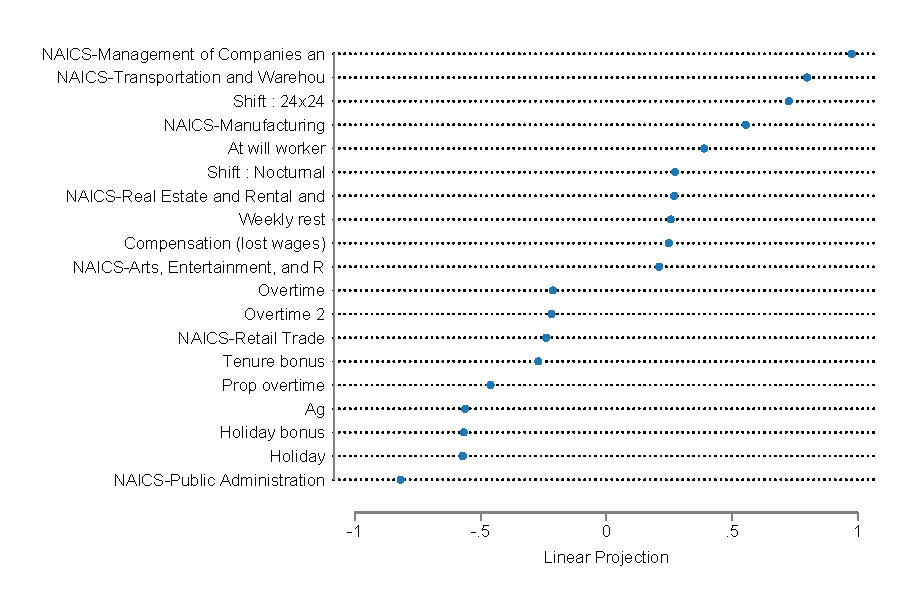
\includegraphics[width=\textwidth]{paper/Figures/coef1_m14.pdf}
    \end{subfigure}     
    \end{center}
     \scriptsize This figure shows the main features and the role they play in each of the above models. We estimate the effect of this features on the predictions made by this models : $\log{\widehat{pr_i}} = \alpha + \beta_j \log{X_{i,j}} + \epsilon$. Note that we are leaving out all but the variable in question. Qualitatively, these betas can be used to assess the elasticity of the prediction function with the features, they can be interpreted as the elasticity of the partial effect of variable $X_{j}$ on the model's prediction.  We only plot the 20 (out of 72) most important features defined as the ones with the biggest estimates in absolute value.  
          %\footnotesize{ \textit{Do file: }  \texttt{coefplots.do}}
\end{figure}


\subsection*{Other issues: Censoring}

All of the models are estimated on a sample of cases filed in 2011 and completed by the end of 2015. The fact that the sample contains only the cases that were resolved could introduce a bias in the prediction of outcomes of ongoing cases. For example, if we are interested in the probability of winning \textit{eventually} and if cases with larger expected payouts take longer to resolve, then excluding the unresolved cases may produce an underestimate of the average payments in all cases.  

We are aware of this bias and it was communicated to the parties when the calculator information was provided. Although we cannot know how large the bias is, we performed two exercises that suggest it is not large. First, we compare characteristics of ongoing cases with those of the historical cases used in the models. In Figure \ref{covariate_distribution} we show that the two sets of cases are similar. The second exercise compares the characteristics of completed and continuing lawsuits within the historical data. To do this we drew a random sample of 956 cases filed in 2011 that were not finished by 2015 (i.e. this represents the complement of our historical dataset). We compare these 956 cases to the completed cases used to develop the models. Figure \ref{FinishedUnfinished} reports the results. There are no significant differences between these two samples, and the magnitude of the measured differences are all very small. 

\begin{figure}[H]
\caption{Covariate distribution comparison : Historical and Phase 1 data}
\label{covariate_distribution}
    \begin{center}
        \begin{subfigure}{0.7\textwidth}
            \caption*{Continuous variables}
            \centering
            \includegraphics[width=0.7\textwidth]{paper/Figures/covariates_continous.tiff}
        \end{subfigure}
        \begin{subfigure}{0.7\textwidth}
            \caption*{Categorical variables}
            \centering
            \includegraphics[width=0.7\textwidth]{covariates_categorical.tiff}
        \end{subfigure}
        \end{center}
          {\scriptsize \textit{Notes: } Covariate distributions comparisons. We compare between -used to calibrate our calculator- and Phase 1 data.  All continuous variables are plotted in logs. Color guide is the same for both variable types. Plots for continuous variables show the p-value of a Kolmogorov–Smirnov test in the subtitle. In the categorical covariates plot, we show significance of a two-sided t-test of differences in means between samples.}
    % {\scriptsize \textit{Script: } \texttt{covariate\_plots.R , covariate\_plots\_hd.R }}
        \end{figure}
        
        
 \begin{figure}[H]
        \caption{Covariate distribution comparison : Historical data: Ended and not ended cases}
        \label{FinishedUnfinished}
        \begin{center}
             \begin{subfigure}{\textwidth}
            \caption*{Continuous variables}
            \centering
            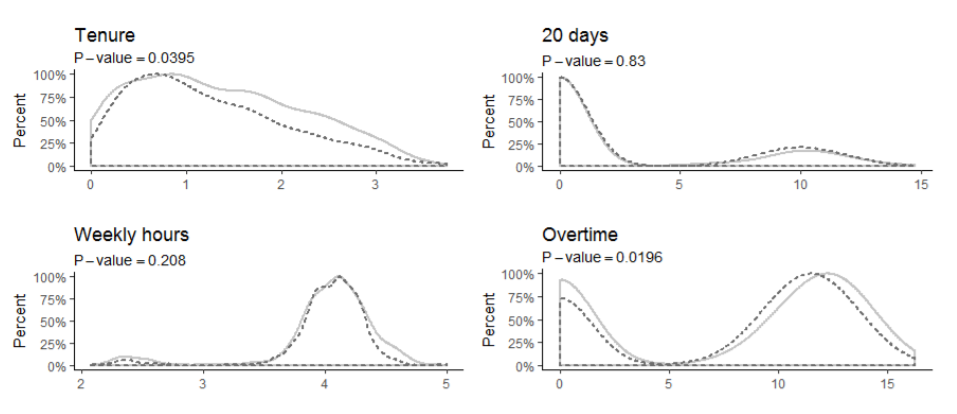
\includegraphics[width=0.7\textwidth]{covariates_hdsample_continous.PNG}
        \end{subfigure}
        \begin{subfigure}{0.7\textwidth}
            \caption*{Categorical variables}
            \centering
            \includegraphics[width=0.7\textwidth]{covariates_hdsample_categorical.tiff}
        \end{subfigure}
    \end{center}
    {\scriptsize \textit{Notes: } Covariate distributions comparisons between historical data cases: ended and not ended after 3 years. All continuous variables are plotted in logs. Color guide is the same for both variable types. Plots for continuous variables show the p-value of a Kolmogorov–Smirnov test in the subtitle. In the categorical covariates plot, we show significance of a two-sided t-test of differences in means between samples.}
    % {\scriptsize \textit{Script: } \texttt{covariate\_plots.R , covariate\_plots\_hd.R }}
\end{figure}


%\begin{figure}[!ht]
%    \caption{Compensation histograms - Historical Data}
%    \label{hist_npv_hd}
%    \begin{center}
%        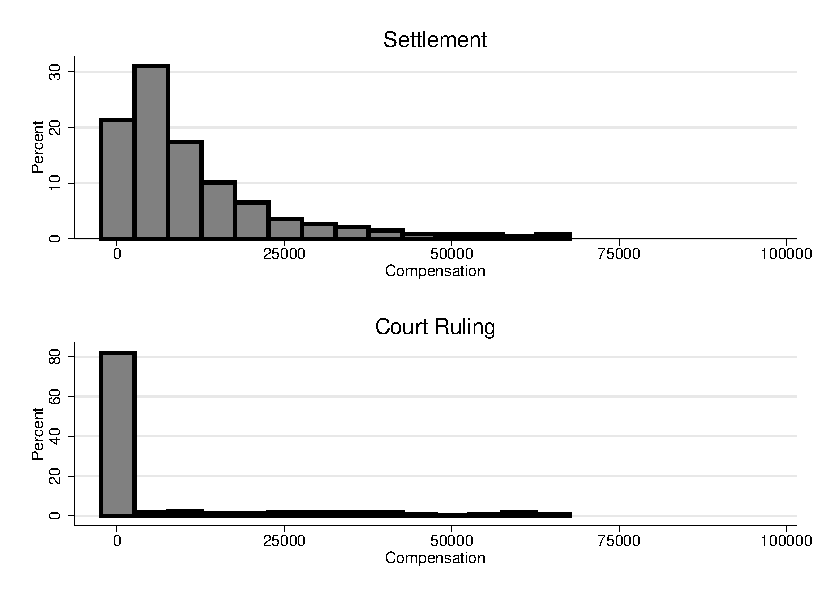
\includegraphics[width=0.5\textwidth]{hist_npv_hd.pdf}
%        \end{center}
%        {\scriptsize \textit{Notes:} Distribution of compensation %in present value at the time of suing with a monthly %interest rate of $3.43$, with a $30$ percent cost, and an %initial fee of MXN\$2000 pesos for private lawyers and %deflated into June 2016 pesos. }
%        % \textit{Do File: } \texttt{histograms\_npv\_hd.do}
%\end{figure}


\FloatBarrier
\newpage
\section*{Appendix B}
\label{appendix_b}
%Isaac Meza
\setcounter{table}{0}
\renewcommand{\thetable}{B.\arabic{table}} 
\setcounter{figure}{0}
\renewcommand{\thefigure}{B.\arabic{figure}} 

\title{\Large{\textbf{The Effect of Agency on Settlement Rates}}}

We aim to write down a simple model that aims to illuminate why agency issues plausibly the underlying cause of the patterns in treatment we find on Tables \ref{Treatment_effects} and \ref{te_bylawyer}. The treatment is effective only when plaintiffs are present to receive it directly. Moreover, this pattern is driven by cases where the plaintiff is represented by a private lawyer. These basic facts could be explained by several models, and we do not claim that the simple and highly stylized framework we write down here is the only way to rationalize them.

Private lawyers almost always receive a share of whatever the plaintiff collects. We should expect the contingency payment contract to align incentives with regard to effort at least partially. We focus instead on differences in incentives over the decision to settle or proceed with the case.  The parties differ in their ability to diversify risks and are also likely to have different discount rates. Our framework focuses on these differences, and shows why they may lead to differences in preferences over taking a certain payoff now (i.e., a settlement) or an uncertain payoff later (i.e., a court judgment). 

 We start with three utility functions, $\left(U_w(x), U_l(x), U_f(x)\right)$, defined over the amount awarded to plaintiffs for the plaintiff ($w$), the plaintiff's lawyer ($l$), and the firms($f$)\footnote{We will assume that $U(0)=0$, $U^{\prime}(x)>0$ and $U^{\prime\prime}(x)\leq 0$, so that $U$ is risk averse or risk neutral. We can think of the 30 percent of any recovery that the plaintiffs' lawyers typically receive as being already reflected in their utility function.}, and subjective distributions $g_k(x)$ for $k=\{w,l,f\}$ for the amount that party $k$ recovers (pays) in a trial. We define the \emph{settlement range} between the plaintiff and defendant as $I_{w,f}:=\left\{x\;\;|\;\;\mathbb{E}_wU_w\leq x\leq\mathbb{E}_fU_f\right\}$, where expectations are taken with respect to $g_k(x)$ and the utility functions incorporate attitudes toward risk over uncertain outcomes. If the utility over outcomes differs for plaintiffs and their lawyers, then we can also define a similar settlement range between firms and plaintiff's lawyers as $I_{l,f}:=\left\{x\;\;|\;\;\mathbb{E}_lU_l\leq x\leq\mathbb{E}_fU_f\right\}$. 

We show three claims that follow from this simple framework.

\begin{claim}
\label{claim1}
Suppose $g_w(x)=g_l(x)=g_f(x):=g(x)$  and 
\[A_{U_w}(x)\geq A_{U_l}(x)\geq A_{U_f}(x)\quad ;\;\forall\;x\in \operatorname{supp} g \]
where $A_{U}(x)-\frac{U^{\prime\prime}(x)}{U^{\prime}(x)}$ is the Arrow-Pratt measure of risk aversion. Suppose further that $U_w^{\prime}(x)\leq U_l^{\prime}(x)\leq U_f^{\prime}(x)$ in a neighbourhood of $0$. Then $\emptyset\neq I_{l,f}\subseteq I_{w,f}$. That is, the worker is more willing to settle than her lawyer.
\end{claim}

\textit{Proof of claim (\ref{claim1}):}
It will suffice to prove that $\mathbb{E}_wU_w\leq \mathbb{E}_lU_l\leq \mathbb{E}_fU_f$. 

Now, 
\begin{align*}
A_{U_w}(x)\geq A_{U_l}(x)\; \Longleftrightarrow & \; \frac{U_w^{\prime\prime}(x)}{U_w^{\prime}(x)}\leq \frac{U_l^{\prime\prime}(x)}{U_l^{\prime}(x)} \\
\Longleftrightarrow \; & \frac{d}{dx}\ln(U_w^{\prime}(x))\leq \frac{d}{dx}\ln(U_l^{\prime}(x))\\
\;\Longleftrightarrow & \int_0^{y}\frac{d}{dx}\ln(U_w^{\prime}(x))dx\leq \int_0^{y}\frac{d}{dx}\ln(U_l^{\prime}(x))dx \;\;\forall\; y\in\;\operatorname{supp}g\\
\Longleftrightarrow \; & \ln(\frac{U_w^{\prime}(y)}{U_w^{\prime}(0)})\leq \ln(\frac{U_l^{\prime}(y)}{U_l^{\prime}(0)})\;\;\forall\; y\in\;\operatorname{supp}g\\
\; \Longleftrightarrow & \frac{U_w^{\prime}(y)}{U_w^{\prime}(0)}\leq \frac{U_l^{\prime}(y)}{U_l^{\prime}(0)}\;\;\forall\; y\in\;\operatorname{supp}g \\
\Longrightarrow \; & U_w^{\prime}(y)\leq U_l^{\prime}(y)\;\;\forall\; y\in\;\operatorname{supp}g
\end{align*}

As $U(0)=V(0)$ the last inequality tells us that
\[U_w(x)\leq U_l(x)\;\;\forall\; x\in\;\operatorname{supp}g\]
 which together with the fact that all parties follow the same subjective distribution leads to 
 \[\mathbb{E}_wU_w\leq \mathbb{E}_lU_l\]
 The other inequality is proved analogously.


Claim 1 says that even with the same subjective $g(x)$ for all parties, if plaintiffs are more risk averse than defendants\footnote{Since the workers typically have much lower incomes and have recently lost a job, and since both the plaintiff's lawyers and the firms typically manage several cases simultaneously, we believe this is a reasonable assumption. With a slightly more complex model, we can get the same result even with the same utility function for the lawyer and the worker, if lawyers are able to diversify across multiple cases. Since, on average, lawyers surveyed in phase 1 reported having more than 100 open cases, we think it is safe to say that lawyers are far more diversified than workers.} then the settlement range between the worker and firm is non empty. Moreover, if the worker is more risk averse than her lawyer, then the settlement range between the firm and the plaintiff's lawyer is a subset of the settlement range between the firm and the plaintiff. Therefore, the worker will be willing to accept some settlement offers that her lawyer will want to reject. The difference in the circumstances governing risk creates a potential conflict of interest between the plaintiff and her own lawyer. 

\begin{claim}
\label{claim2}
Assume additionally that $g^o_w \succeq_{FOSD} g_w$. Then $I_{w^o,f} \subseteq I_{w,f}$. That is, overconfidence shrinks the settlement range.
\end{claim}

\textit{Proof of claim (\ref{claim2}):}
As $g^o_w$ first-order stochastically dominates $g_w$ then 
\[\mathbb{E}_{g^o_w}U\geq \mathbb{E}_{g_w}U\]
for all weakly increasing $U$. From this the claim follows directly.


Claim 2 relaxes the assumption of the same expectations over outcomes to allow for overconfidence. We show that if the worker is overconfident (i.e. $g_w^o$ first-order stochastically  dominates $g_w$) then the settlement range shrinks. Indeed, if the parties are sufficiently optimistic, the settlement range will be empty. Our surveys in phase 3 indicate that workers are wildly optimistic before filing a case. Because most workers are suing for the first time, while their lawyers have typically handled a large number of cases, the lawyers have the ability to guide workers toward realistic expectations or maintain their initial overconfidence. The misalignment between the worker and her lawyer generated by Claim 1 gives an incentive for the lawyer to inflate the expectations of the worker. 

\begin{claim}
\label{claim3}
Let the worker have a prior distribution $g_w$, and let the calculator be a signal with distribution $S$. Suppose further that the signal satisfies  $g_w \succeq_{FOSD} S$ and that the agent is Bayesian. If we denote the posterior by $\hat{g}_w$, then $I_{w,f} \subseteq I_{\hat{w},f}$. That is, after updating the settlement range increases.
\end{claim}
%\footnote{We say that the agent is Bayesian if he follow a \emph{Bayesian rule} according to definition in \textit{Shmaya \& Yariv. Foundations for Bayesian Updating.}}

\textit{Proof of claim (\ref{claim3}):}
We will prove that  $g_w \succeq_{FOSD} \hat{g}_w \succeq_{FOSD} S$, combining this fact with Claim \ref{claim2} will yield the desired result.

As the agent is Bayesian, then by Theorem 1 in \textit{Foundations for Bayesian Updating} we can write $\hat{g}_w=\alpha g_w+(1-\alpha)S$ for some $\alpha\in [0,1]$. Then,

\[\mathbb{E}_{\hat{g}_w}U=(1-\alpha)\mathbb{E}_{g_w}U+\alpha \mathbb{E}_{S}U\leq(1-\alpha)\mathbb{E}_{S}U+\alpha \mathbb{E}_{S}U= \mathbb{E}_{S}U\]
for all weakly increasing $U$. As $S$ is dominated by $g_w$, this yields the desired inequality.


Claim 3 introduces the calculator as a signal received by Bayesian updaters, and shows that when initially overconfident workers get the calculator, their settlement range increases to $\hat{I}_{w,f}$, leading to more settlements.

The effect of the three claims can be illustrated in the following figure, which shows the effect of overconfidence and differences in the ability to diversify risk on the settlement range over which parties might bargain a resolution to the case.  

\begin{figure}[H]
   \caption{Illustration of claims}
   \label{figure}
\begin{center}
 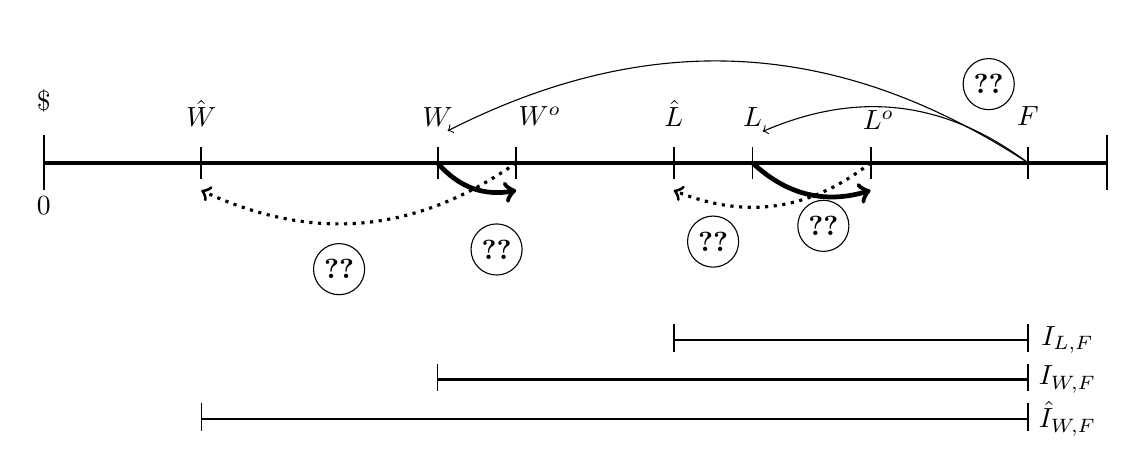
\begin{tikzpicture}
    \draw[line width=0.5mm] (0,0) -- (13.5,0) node [below] {};
    \foreach \x in {0,13.5}
    \draw[line width=0.3mm] (\x, 0.35) -- node[pos=-0.25] (point\x) {} (\x, -0.35);
    
    \foreach \x in {2, 5, 6, 8, 9, 10.5, 12.5}
    \draw[line width=0.25mm] (\x, 0.2) -- node[pos=-0.35] (point\x) {} (\x, -0.2);
    % node's content --- access them as point1...point5
    \path (point0) node [above] {$\$$};
    \path (0,-0.3) node [below] {$0$};
    \path (point2) node [above] {$\hat{W}$};
    \path (point5) node [above] {$W$};
    \path (6.3,0.35) node [above] {$W^o$};
    \path (point8) node [above] {$\hat{L}$};
    \path (point9) node [above] {$L$};
    \path (10.6,0.3) node [above] {$L^o$};
    \path (12.5,0.35) node [above] {$F$};
    
    \path (12.5,0) edge[black, bend right, ->] (point9);
    \path (12.5,0) edge[black, bend right, ->] (point5);
    \draw (12,1) node[circle,draw, inner sep=2pt](c1) {$\ref{claim1}$};
    
    \path (5,0) edge[black, line width=0.6mm, bend right, below, ->] (6,-0.35);
    \draw (5.75,-1.1) node[circle,draw, inner sep=2pt](c2) {$\ref{claim2}$};
    
    \path (9,0) edge[black, line width=0.6mm, bend right, below, ->] (10.5,-0.35);
    \draw (9.9,-0.8) node[circle,draw, inner sep=2pt](c2) {$\ref{claim2}$}; 
    
    \path (6,0) edge[black, line width=0.4mm, dotted, bend left, below, ->] (2,-0.35);
    \path (3.75,-1.35) node[circle,draw, inner sep=2pt]  {$\ref{claim3}$};

    
    \path (10.5,0) edge[black, line width=0.4mm, dotted, bend left, below, ->] (8,-0.35);
    \draw (8.5,-1.0) node[circle,draw, inner sep=2pt] {$\ref{claim3}$};  

    
    \draw[line width=0.3mm] (8,-2.25) -- (12.5,-2.25) node [below] {};
    \foreach \x in {8,12.5}
    \draw[line width=0.2mm] (\x, -2.05) -- node[pos=-0.25] {} (\x, -2.4);
    \path (13,-2.25) node  {$I_{L,F}$};
    
    \draw[line width=0.3mm] (5,-2.75) -- (12.5,-2.75) node [below] {};
    \foreach \x in {5,12.5}
    \draw[line width=0.2mm] (\x, -2.55) -- node[pos=-0.25] {} (\x, -2.9);
    \path (13,-2.75) node  {$I_{W,F}$}; 
    
    
    \draw[line width=0.3mm] (2,-3.25) -- (12.5,-3.25) node [below] {};
    \foreach \x in {2,12.5}
    \draw[line width=0.2mm] (\x, -3.05) -- node[pos=-0.25] {} (\x, -3.4);
    \path (13,-3.25) node  {$\hat{I}_{W,F}$}; 
    
  \end{tikzpicture}
 \end{center}

\scriptsize
    \textit{Notes:} 
    To simplify the notation we will simply write the subindex $i\in \lbrace W, L , F\rbrace$ to denote $\mathbb{E}_iU_i$. The arrows describe the conclusion on each of the claims: Initially with the same subjective probability but with different degrees of risk aversion, the expected utility of the different parties differ. This is Claim \ref{claim1}. Claim \ref{claim2} tells us that for overconfident individuals (here denoted by $W^o$), their expected utility increases. Finally, Claim \ref{claim3} is about the updating process for lawyers and workers, assuming that the calculator reduces the overconfidence. The conclusion is that after updating, the settlement range increases.  The last intervals denote the \emph{settlement range}, the first one for the lawyer and the last two before and after updating, when the employee is present. 
\end{figure} 









\FloatBarrier
%%%%%%%%%%%%%%%%%%%%%%%%%%%%%%%%%%%%%%%%%%%%%%%
%           APPENDIX
%%%%%%%%%%%%%%%%%%%%%%%%%%%%%%%%%%%%%%%%%%%%%%%

% APPENDIX TABLES
\newpage
\section*{Appendix C}
\label{appendix_c}

\setcounter{table}{0}
\renewcommand{\thetable}{C.\arabic{table}} 
\setcounter{figure}{0}
\renewcommand{\thefigure}{C.\arabic{figure}} 

\subsection{Tables}

\begin{table}[!ht]
    \caption{Amount asked (log), amount won (log), and probability of winning - Historic Data}
    \label{Table_Reg_winnings_log}
    \begin{center}

        \scriptsize{% Table generated by Excel2LaTeX from sheet 'TableReg1_log'
\begin{tabular}{lcccc}
\toprule
      & \multicolumn{4}{c}{Panel A : All cases} \\
\midrule
\midrule
      & Total asked & Amount Won & Won/asked & Prob winning \\
\midrule
\midrule
Public Lawyer & -0.62*** & 0.0011 & 0.055** & 1.65 \\
      & (0.033) & (0.22) & (0.024) & (2.33) \\
Constant & 2.76*** & 5.48*** & 1.06*** & 75.6*** \\
      & (0.19) & (0.97) & (0.10) & (9.67) \\
      &       &       &       &  \\
\midrule
Observations & 4866  & 4866  & 4866  & 4866 \\
BVC   & YES   & YES   & YES   & YES \\
Dummy Industry & YES   & YES   & YES   & YES \\
R-squared & 0.74  & 0.036 & 0.043 & 0.020 \\
DepVarMean & 11.7  & 6.40  & 0.21  & 65.3 \\
\midrule
\midrule
      &       &       &       &  \\
\midrule
      & \multicolumn{4}{c}{Panel B : Settlement} \\
\midrule
\midrule
      & Total asked & Amount Won & Won/asked & Prob winning \\
\midrule
\midrule
Public Lawyer & -0.67*** & -0.20*** & 0.087*** & 0.018 \\
      & (0.041) & (0.053) & (0.020) & (0.37) \\
Constant & 2.63*** & 6.59*** & 1.52*** & 99.4*** \\
      & (0.25) & (0.31) & (0.11) & (2.15) \\
      &       &       &       &  \\
\midrule
Observations & 3077  & 3077  & 3077  & 3077 \\
BVC   & YES   & YES   & YES   & YES \\
Dummy Industry & YES   & YES   & YES   & YES \\
R-squared & 0.74  & 0.37  & 0.11  & 0.0068 \\
DepVarMean & 11.7  & 9.70  & 0.27  & 99.6 \\
\midrule
\midrule
      &       &       &       &  \\
\midrule
      & \multicolumn{4}{c}{Panel C: Court ruling} \\
\midrule
\midrule
      & Total asked & Amount Won & Won/asked & Prob winning \\
\midrule
\midrule
Public Lawyer & -0.44*** & -0.22 & 0.027 & -0.59 \\
      & (0.12) & (0.81) & (0.29) & (7.59) \\
Constant & 2.14*** & 0.63  & 1.86** & 7.23 \\
      & (0.68) & (3.14) & (0.84) & (27.5) \\
      &       &       &       &  \\
Observations & 422   & 422   & 422   & 422 \\
BVC   & YES   & YES   & YES   & YES \\
Dummy Industry & YES   & YES   & YES   & YES \\
R-squared & 0.78  & 0.13  & 0.065 & 0.13 \\
DepVarMean & 11.7  & 2.74  & 0.37  & 24.2 \\
\bottomrule
\bottomrule
\end{tabular}%
}
    \end{center}
    \scriptsize
%\begin{figurenotes}
   This table shows OLS regressions of log total amount asked in the initial labor suit, the amount actually won, the ratio of these two, and the probability of the worker recovering a positive amount. Panel A includes all our historical data files (i.e. for all types of case ending), Panel B focuses on cases ending in settlement, and Panel C on those ending in court ruling. All regressions control for our basic variable controls (gender, at will worker, tenure at the firm, daily wage, weekly hours worked), as well as industry dummies in which firm operates in. We have 4866 observations instead of 5005 since there are some missing values in the controls.
     %\textit{Do file: } \texttt{reg_amount.do}
%   \end{figurenotes}     
\end{table}


\begin{table}[!ht]
    \caption{Balance of casefiles having negative recovery amount.}
    \label{negative_returners}
    \begin{center}
    \scriptsize{% Table generated by Excel2LaTeX from sheet 'negative_returners_balance'
\begin{tabular}{lccccc}
\toprule
      & Gender & At will worker & Tenure & Daily wage & Weekly hours \\
\midrule
\midrule
      & (1)   & (2)   & (3)   & (4)   & (5) \\
\midrule
\midrule
Negative NPV & -0.035** & -0.034 & -0.006*** & -0.000 & 0.002*** \\
      & (0.014) & (0.028) & (0.001) & (0.000) & (0.001) \\
Constant & 0.417*** & 0.404*** & 0.428*** & 0.402*** & 0.279*** \\
      & (0.017) & (0.016) & (0.017) & (0.016) & (0.035) \\
      &       &       &       &       &  \\
\midrule
Observations & 4503  & 4492  & 4470  & 4484  & 4425 \\
R-squared & 0.014 & 0.013 & 0.017 & 0.013 & 0.017 \\
F stat & 13.022 & 12.109 & 15.139 & 11.902 & 15.373 \\
Court dummies & YES   & YES   & YES   & YES   & YES \\
\bottomrule
\bottomrule
\end{tabular}%
}
    \end{center}
     \scriptsize
    \textit{Notes:} Each column regresses a characteristic of the case against a dummy variable indicating that the plaintiff recovered an amount less than the MXN\$2000 initial filing fee. The sample is all cases from the historical data using private lawyers.  
         
    %\textit{Do file: } \texttt{negReturnHD.do}
\end{table}


%\begin{table}[!ht]
%   \caption{Treatment description - Phase 1}
%    \label{treatment_description}
%    \begin{center}
%    \scriptsize{\input{paper/Tables/Experiment_description2.tex}}
%    \end{center}
%     \scriptsize
%    \textit{Notes:} This is a short description of the kind of treatment received by each treatment group.
%\end{table}

%\begin{table}[!ht]
%    \caption{Settlements against duration - historical Data}
%    \label{settlement_time}
%    \begin{center}
%    \scriptsize{% Table generated by Excel2LaTeX from sheet 'settlementq_time'
\begin{tabular}{lcccccc}
\toprule
      & \multicolumn{2}{c}{Settlement amount} & \multicolumn{2}{c}{Settlement amt discounted} & \multicolumn{2}{c}{Calculator prediction} \\
\midrule
\midrule
      & (1)   & (2)   & (3)   & (4)   & (5)   & (6) \\
\midrule
\midrule
Months  & 1202.9*** &       & -166.3** &       & 180.0*** &  \\
      & (166.8) &       & (70.37) &       & (30.82) &  \\
2 Quintil &       & 4052.7** &       & 1754.3 &       & 1576.3*** \\
      &       & (1859.3) &       & (1676.1) &       & (460.2) \\
3 Quintil &       & 1622.4 &       & -1767.8 &       & 1451.0** \\
      &       & (2015.3) &       & (1705.6) &       & (565.7) \\
4 Quintil &       & 8663.2*** &       & 44.58 &       & 3029.1*** \\
      &       & (2348.7) &       & (1808.5) &       & (595.2) \\
5 Quintil &       & 21982.6*** &       & -3474.0* &       & 3990.9*** \\
      &       & (3299.9) &       & (1882.0) &       & (718.8) \\
Constant  & 10907.8*** & 15396.9*** & 15841.8*** & 14649.2*** & 9544.0*** & 9331.9*** \\
      & (4229.2) & (4326.9) & (2953.9) & (3018.0) & (1031.9) & (1076.7) \\
      &       &       &       &       &       &  \\
\midrule
Observations  & 3080  & 3080  & 3080  & 3080  & 3081  & 3081 \\
R-squared & 0.24  & 0.23  & 0.22  & 0.22  & 0.66  & 0.65 \\
BVC   & YES   & YES   & YES   & YES   & YES   & YES \\
\bottomrule
\bottomrule
\end{tabular}%
}
%    \end{center}
%     \scriptsize
%    \textit{Notes:} 
%    This table focuses on the sample of cases from the historical data (HD) that settled at any point in time (3080 cases out of 5005). Each column is a different regression. All regressions control for the basic variables of the case (BVC) which are described in Panel B of Table 1. Columns 1 and 2 have as a dependent variable the settlement amount in pesos the worker actually got in the settlement. Column 1 regresses this amount on a counter for the number of months that elapsed from the initial filing until the settlement. Column 2 breaks this elapsed time in quintiles dummies. Columns 3 and 4 discount the peso amount at a 3.43 monthly rate. This rate was calculated by matching our sample to that of the MxFls survey and obtaining the elicited time discount rate for similar individuals (using gender, age, education, daily wage, and weekly hours), and taking the median. Columns 5 and 6 use the prediction from our ``calculator'', that is, the amount they would get on average given the initial case characteristics, with no discounting.
    %\textit{Do file: } \texttt{settlementq\_time.do}
%\end{table}

\begin{table}[!ht]
    \caption{Balance regression on characteristics conditional on employee present}
    \label{ep_balance}
    \begin{center}
    \scriptsize{% Table generated by Excel2LaTeX from sheet 'ep_balance'
\begin{tabular}{rccccc}
\toprule
      & Control & Calculator & Observations & R-squared & p-value (calculator = 0) \\
\midrule
\midrule
\multicolumn{1}{l}{Public Lawyer} & 0.223*** & 0.034 & 312   & 0.042 & 0.492 \\
      & (0.043) & (0.049) &       &       &  \\
\multicolumn{1}{l}{Gender} & 0.162* & -0.256** & 312   & 0.080 & 0.0395 \\
      & (0.0890) & (0.121) &       &       &  \\
\multicolumn{1}{l}{At will worker} & 0.0197 & -0.0351 & 312   & 0.049 & 0.742 \\
      & (0.0965) & (0.106) &       &       &  \\
\multicolumn{1}{l}{Tenure} & 0.189 & -0.286* & 306   & 0.068 & 0.0814 \\
      & (0.133) & (0.161) & .     &       &  \\
\multicolumn{1}{l}{Daily wage} & 0.0659 & -0.0975 & 307   & 0.006 & 0.493 \\
      & (0.141) & (0.141) &       &       &  \\
\multicolumn{1}{l}{Weekly hours} & 0.0230 & -0.0203 & 306   & 0.136 & 0.863 \\
      & (0.0755) & (0.117) &       &       &  \\
\bottomrule
\bottomrule
\end{tabular}%
}
    \end{center}
     \scriptsize
    \textit{Notes:} The table shows results of regressions with the specification $y_i = \alpha_t + \beta T_i + \epsilon_{i}$. The sample is limited to the cases in which the plaintiff was present at the hearing.  Each columns represents a different regression with the indicated independent variable. The regressions all include subcourt fixed effects. 
         
    %\textit{Do file: } \texttt{ep\_balance.do}
\end{table}




\begin{table}[!ht]
    \caption{Employee presence}
    \label{pactor_reg}
    \begin{center}
    \scriptsize{% Table generated by Excel2LaTeX from sheet 'pactor_reg'
\begin{tabular}{lccc}
\toprule
      & \multicolumn{3}{c}{Employee Present} \\
\midrule
\midrule
      & Phase 1 & Phase 2 & Phase 1/2 \\
\midrule
\midrule
      & (1)   & (2)   & (3) \\
\midrule
\midrule
Female & -0.066* & 0.000 & -0.023 \\
      & (0.035) & (0.023) & (0.019) \\
Public Lawyer & 0.317*** & 0.508*** & 0.416*** \\
      & (0.066) & (0.059) & (0.045) \\
At will worker & -0.063 & 0.013 & -0.016 \\
      & (0.049) & (0.042) & (0.032) \\
Tenure (years) & 0.004 & 0.005** & 0.005*** \\
      & (0.003) & (0.002) & (0.002) \\
Daily wage & -0.000 & -0.000 & -0.000 \\
      & (0.000) & (0.000) & (0.000) \\
Weeky hours & -0.002** & -0.003*** & -0.003*** \\
      & (0.001) & (0.001) & (0.001) \\
Age   &       & -0.001 &  \\
      &       & (0.003) &  \\
Constant & 0.313*** & 0.303*** & 0.298*** \\
      & (0.062) & (0.066) & (0.045) \\
      &       &       &  \\
\midrule
Observations & 520   & 1026  & 1546 \\
R-squared & 0.090 & 0.124 & 0.105 \\
DepVarMean & 0.208 & 0.183 & 0.191 \\
p-value & 0.000 & 0.000 & 0.000 \\
p-value w/o PL & 0.014 & 0.001 & 0.000 \\
\bottomrule
\bottomrule
\end{tabular}%
}
    \end{center}
    \scriptsize
    \textit{Notes:} OLS of employee presence against basic variable controls as predictors. Last two rows shows the p-value testing the quality of all basic variables ( \& without public lawyer) respectively.
     
    % \textit{Do file: } \texttt{pEmployeePresence.do}
\end{table}

\begin{table}[!ht]
    \caption{Expectations Relative to Prediction}
    \label{prediction_cases}
   % \scriptsize{% Table generated by Excel2LaTeX from sheet 'prediction_cases_pooled'
\begin{tabular}{lcccc}
\toprule
      & \multicolumn{2}{c}{Expectation} & \multicolumn{2}{c}{Relative OC} \\
\midrule
\midrule
      & Probability & Amount & Probability & Amount \\
\midrule
      & (1)   & (2)   & (3)   & (4) \\
\midrule
\midrule
Employee's Lawyer & 4.52  & 5902.2 & 0.22  & -0.097 \\
      & (3.46) & (12555.8) & (0.14) & (0.53) \\
Firm's Lawyer & -27.4*** & -27573.0** & -0.96*** & -0.38 \\
      & (3.34) & (12083.0) & (0.13) & (0.50) \\
Constant & 75.0*** & 74788.7*** & 1.64*** & 0.73* \\
      & (2.86) & (10219.5) & (0.11) & (0.43) \\
      &       &       &       &  \\
\midrule
Observations & 2214  & 1859  & 1952  & 1632 \\
File Fixed Effects & YES   & YES   & YES   & YES \\
R-squared & 0.83  & 0.89  & 0.96  & 0.89 \\
p-value:Emp Law & 0     & 0     & 0     & 0 \\
p-value:Firm Law & 0     & 0     & 0     & 0.1 \\
\bottomrule
\bottomrule
\end{tabular}%
}
   \begin{center}
    \scriptsize{% Table generated by Excel2LaTeX from sheet 'prediction_cases_pooled_panels'
\begin{tabular}{lccccc}
\toprule
\multicolumn{6}{c}{\textbf{Panel A}} \\
\midrule
      & \multicolumn{2}{c}{Expectation} &       & \multicolumn{2}{c}{Relative OC} \\
\cmidrule{2-3}\cmidrule{5-6}      & Probability & Amount &       & Probability & Amount \\
\midrule
      & (1)   & (2)   &       & (3)   & (4) \\
\midrule
\midrule
Employee's Lawyer ($\beta_1$) & 0.070 & 11410.9 &       & 0.28  & -0.17 \\
      & (0.044) & (13314.9) &       & (0.18) & (0.71) \\
Firm's Lawyer ($\beta_2$) & -0.25*** & -21804.2* &       & -0.86*** & -0.51 \\
      & (0.042) & (12614.9) &       & (0.17) & (0.67) \\
Constant (employee $\alpha$) & 0.74*** & 66755.3*** &       & 1.70*** & 1.00* \\
      & (0.036) & (10791.5) &       & (0.15) & (0.58) \\
      &       &       &       &       &  \\
\midrule
Observations & 1274  & 1104  &       & 1177  & 1032 \\
File Fixed Effects & YES   & YES   &       & YES   & YES \\
R-squared & 0.79  & 0.91  &       & 0.96  & 0.89 \\
p-value:Emp Law & 0     & 0     &       & 0     & 0 \\
p-value:Firm Law & 0     & 0     &       & 0     & 0.04 \\
\midrule
\midrule
      &       &       &       &       &  \\
\midrule
\multicolumn{6}{c}{\textbf{Panel B}} \\
\midrule
      & \multicolumn{2}{c}{Expectation} &       & \multicolumn{2}{c}{Relative OC} \\
\cmidrule{2-3}\cmidrule{5-6}      & Probability & Amount &       & \multicolumn{2}{c}{Amount} \\
\midrule
      & (1)   & (2)   &       & (3)   & (4) \\
\midrule
\midrule
Mean  & 0.885*** & 58,077*** &       & 1.713*** & 1.315*** \\
      & (0.00288) & (1,794) &       & (0.0729) & (0.0619) \\
Standar deviation & 0.166 & 74471 &       & 3.026 & 2.570 \\
      &       &       &       &       &  \\
\midrule
Observations & 3,330 & 1,723 &       & 1,723 & 1,723 \\
Ignores prob. (\%) & 13.08 &       &       &       &  \\
Standard deviation & 0.166 & 74471 &       & 3.026 & 2.570 \\
Reference &       &       &       & Mid prediction & Max prediction \\
\bottomrule
\bottomrule
\end{tabular}%
}
    \end{center}
% \begin{figurenotes}
    \scriptsize
\textit{Notes:} The table regresses measures of expectation elicited in the baseline survey on dummies of who is the respondent of the survey. For some cases we could elicit the expectation of more than one party (employee, employee's lawyer, firm's lawyer). The omitted variable is the employee dummy, so the interpretation of the employee's lawyer and firm's lawyer coefficients are relative to the employee who is captured in the constant. It combines two phases in one singled pooled dataset. Each column represents a different regression. The first column use elicited probability of winning as a dependent variable. The exact question is: \textit{``How likely is it that you will win the lawsuit if it ends in a court judgment?''}. The second column use the peso amount (undiscounted) that they expect to recover conditional on winning. The exact wording of the survey question is: \textit{``in case you win the lawsuit, what amount are you most likely to win?''}.  All columns include casefile fixed effects, avoiding the comparison across casefiles. The bottom of the table present the p-values of two null hypothesis:  $\alpha + \beta_1=0$, and $\alpha + \beta_2=0$, telling us whether the employee's lawyer, or firm's lawyer are more or less confident. Last 2 columns use a measure of ``overconfidence'', which compares the subjective expectation vs the personalized calculator prediction. Relative OC is computed as $\frac{expectation-prediction}{prediction}$, where expectation refers to the expectation measured in the baseline survey.
    %\textit{Do file: } \texttt{prediction\_cases\_pooled.do, ExpectationsFromP3forPrediction_cases_pooles_panelB.do}
 %  \end{figurenotes}    
\end{table}

%Old version of other PSM tabel?
%\begin{table}[!ht]
%    \caption{Comparison of settlement amounts}
%    \label{match_table_lr}
%     \begin{center}
%      \centering
%        \scriptsize{% Table generated by Excel2LaTeX from sheet 'NN_match_lr'
\begin{tabular}{lcccc|cc}
\toprule
\multicolumn{7}{c}{Treatment effect. Nearest-neighbor matching} \\
\midrule
\midrule
      & \multicolumn{6}{c}{Phase 1/2} \\
\midrule
\midrule
      & \multicolumn{4}{c|}{Variable matching} & \multicolumn{2}{c}{PSM} \\
\midrule
\midrule
      & (1)   & (2)   & (3)   & (4)   & (5)   & (6) \\
\midrule
ATE   & 6154  & 8867** & 6893* & 9852** & 8079* & 11829** \\
      & (5303) & (4302) & (5310) & (4328) & (6691) & (5345) \\
\% ATE & 81    & 116   & 90    & 129   & 106   & 155 \\
Baseline mean & \multicolumn{6}{c}{7622} \\
Obs   & \multicolumn{6}{c}{89} \\
Obs HD & \multicolumn{6}{c}{414} \\
Bias adjustment & NO    & NO    & YES   & YES   & -     & - \\
Matches & [1-1] & [1-3] & [1-1] & [1-3] & [1-1] & [1-3] \\
\bottomrule
\bottomrule
\end{tabular}%
}
%    \end{center}%
%  \scriptsize
%    \textit{Notes:}
 %  This table is a robustness check considering all cases settled up to December 2018, contrary to cases settled on the same day as Table \ref{match_table}.  See the notes to \ref{match_table} for further details. 
 
   %\textit{Do file: } \texttt{settlement\_conciliator\_matching\_lr.do}
%\end{table}

\begin{table}[!ht]
    \caption{First stage and robustness for the control function regression}
    \label{table_fs_cf}
    \begin{center}
    \scriptsize{% Table generated by Excel2LaTeX from sheet 'fs_treatment_effects'
\begin{tabular}{lcccccccccc}
\toprule
      & \multicolumn{7}{c}{Settlement}                        &       & \multicolumn{2}{c}{Emp present} \\
\cmidrule{2-8}\cmidrule{10-11}      & Probit &       & \multicolumn{2}{c}{OLS} &       & \multicolumn{2}{c}{Probit} &       & OLS   & Probit \\
\cmidrule{2-2}\cmidrule{4-5}\cmidrule{7-8}\cmidrule{10-11}      & (1)   &       & (2)   & (3)   &       & (4)   & (5)   &       & (6)   & (7) \\
\midrule
\midrule
Calculator  & 0.121 &       &       &       &       &       &       &       & 0.0288 & 0.108 \\
      & (0.0950) &       &       &       &       &       &       &       & (0.0175) & (0.0680) \\
Emp present (EP) & 0.723*** &       &       &       &       &       &       &       &       &  \\
      & (0.163) &       &       &       &       &       &       &       &       &  \\
Calculator\#EP & 0.257 &       &       &       &       &       &       &       &       &  \\
      & (0.189) &       &       &       &       &       &       &       &       &  \\
\multicolumn{1}{r}{9:30} &       &       & -0.0496 & -0.0397 &       & -0.218 & -0.213 &       & -0.0410 & -0.133 \\
      &       &       & (0.0410) & (0.0389) &       & (0.168) & (0.227) &       & (0.0401) & (0.138) \\
\multicolumn{1}{r}{10:00} &       &       & -0.0604* & -0.0130 &       & -0.279** & -0.0755 &       & -0.0878*** & -0.326*** \\
      &       &       & (0.0312) & (0.0295) &       & (0.135) & (0.167) &       & (0.0317) & (0.115) \\
\multicolumn{1}{r}{10:30} &       &       & -0.0471 & -0.0423 &       & -0.226 & -0.272 &       & -0.0474 & -0.157 \\
      &       &       & (0.0398) & (0.0389) &       & (0.159) & (0.220) &       & (0.0376) & (0.131) \\
\multicolumn{1}{r}{11:00} &       &       & -0.0744** & -0.0311 &       & -0.354** & -0.189 &       & -0.0649* & -0.224* \\
      &       &       & (0.0321) & (0.0298) &       & (0.141) & (0.172) &       & (0.0334) & (0.121) \\
\multicolumn{1}{r}{11:30} &       &       & -0.0904** & -0.0440 &       & -0.412** & -0.264 &       & -0.129*** & -0.503*** \\
      &       &       & (0.0414) & (0.0417) &       & (0.176) & (0.218) &       & (0.0406) & (0.174) \\
\multicolumn{1}{r}{12:00} &       &       & -0.0648* & -0.0248 &       & -0.301** & -0.182 &       & -0.0419 & -0.138 \\
      &       &       & (0.0373) & (0.0380) &       & (0.152) & (0.201) &       & (0.0353) & (0.119) \\
\multicolumn{1}{r}{12:30} &       &       & 0.306** & 0.293* &       & 0.672* & 0.654 &       & -0.0142 & -0.0297 \\
      &       &       & (0.137) & (0.155) &       & (0.395) & (0.427) &       & (0.122) & (0.435) \\
      &       &       &       &       &       &       &       &       &       &  \\
\midrule
Observations & 1700  &       & 1723  & 1401  &       & 1700  & 1348  &       & 1732  & 1732 \\
R-squared & 0.149 &       & 0.080 & 0.101 &       & 0.0870 & 0.119 &       & 0.037 & 0.0427 \\
Control Mean & \multicolumn{7}{c}{0.116}                             &       & \multicolumn{2}{c}{0.174} \\
$H_0 : Z=0$ (p-value) &       &       & 0.0323 & 0.191 &       & 0.0331 & 0.202 &       & 0.0670 & 0.0844 \\
Conditional on EP=0 &       &       &       & \checkmark &       &       & \checkmark &       &       &  \\
\bottomrule
\bottomrule
\end{tabular}%
}
    \end{center}
     \scriptsize
    \textit{Notes:} The first column repeats the regression in column 5 of \ref{Treatment_effects} using a probit specification rather than a linear probability model. Column (2) is a `reduced form' OLS regression, and column (3) conditions on employee \emph{not} being present. This serves as a test that time of the hearing does not affect settlement for reasons other than the plaintiff's presence. In the bottom panel we included the p-value for the null that the instrumental variables are equal to zero. Columns (4)-(5) are analogous to columns(2)-(3) but with a probit specification. The sixth column is a OLS first stage for employee present, and column (7) is the probit FS used in the control function of table \ref{Treatment_effects}. See the notes to \ref{Treatment_effects} for further details. 
         
    %\textit{Do file: } \texttt{fs_treatment_effects.do}
\end{table}

% \begin{table}[!ht]
%     \caption{Presence of each party at time of hearing}
%     \label{table_fs_cf}
%     \begin{center}
%     \scriptsize{% Table generated by Excel2LaTeX from sheet 'presence_time_hearing'
\begin{tabular}{lccc}
\toprule
      & Emp present & Employee's Lawyer & Defendant \\
\midrule
      & (1)   & (2)   & (3) \\
\midrule
\midrule
\multicolumn{1}{r}{9:30} & -0.0387 & -0.0438 & -0.0236 \\
      & (0.0400) & (0.0352) & (0.0356) \\
\multicolumn{1}{r}{10:00} & -0.0877*** & 0.00589 & -0.0555 \\
      & (0.0329) & (0.0254) & (0.0347) \\
\multicolumn{1}{r}{10:30} & -0.0503 & -0.0146 & -0.0692* \\
      & (0.0373) & (0.0317) & (0.0406) \\
\multicolumn{1}{r}{11:00} & -0.0677* & -0.0177 & -0.0730** \\
      & (0.0346) & (0.0282) & (0.0371) \\
\multicolumn{1}{r}{11:30} & -0.128*** & -0.0374 & -0.0789 \\
      & (0.0402) & (0.0387) & (0.0487) \\
\multicolumn{1}{r}{12:00} & -0.0279 & 0.00838 & -0.150*** \\
      & (0.0358) & (0.0281) & (0.0419) \\
\multicolumn{1}{r}{12:30} & -0.0433 & 0.114*** & -0.0365 \\
      & (0.121) & (0.0195) & (0.136) \\
Constant (9:00) & 0.243*** & 0.886*** & 0.837*** \\
      & (0.0275) & (0.0195) & (0.0235) \\
      &       &       &  \\
\midrule
Observations & 1732  & 1732  & 1732 \\
R-squared & 0.009 & 0.004 & 0.011 \\
DepVarMean & 0.186 & 0.876 & 0.773 \\
F p-value & 0.0614 & 1.49e-35 & 0.0487 \\
\bottomrule
\bottomrule
\end{tabular}%
}
%     \end{center}
%      \scriptsize
%     \textit{Notes:} This table shows the correlation between attendance to hearing of each party involved and the time of hearing.
         
%     %\textit{Do file: } \texttt{presence\_time\_hearing.do}
% \end{table}



\begin{table}[!ht]
    \caption{Time of hearing balance table}
    \label{pactor_balance}
    \begin{center}
    \scriptsize{% Table generated by Excel2LaTeX from sheet 'balance_instrument'
\begin{tabular}{lcccccc}
\toprule
      & Tenure & Public Lawyer & \% severance pay & Daily wage & \% tenure bonus & Entitlement \\
\midrule
      & (1)   & (2)   & (3)   & (4)   & (5)   & (6) \\
\midrule
\midrule
\multicolumn{1}{r}{9:30} & -0.346 & 0.0145 & -0.0666* & 6.814 & -0.0151 & 8909.1 \\
      & (0.623) & (0.0228) & (0.0391) & (91.44) & (0.0428) & (10278.3) \\
\multicolumn{1}{r}{10:00} & -0.648 & 0.0374* & -0.0600** & 81.40 & -0.0328 & 11390.7 \\
      & (0.445) & (0.0204) & (0.0298) & (92.32) & (0.0318) & (9100.5) \\
\multicolumn{1}{r}{10:30} & -0.596 & 0.0325 & -0.00204 & -13.54 & 0.0265 & 1243.9 \\
      & (0.498) & (0.0244) & (0.0370) & (88.12) & (0.0342) & (8802.9) \\
\multicolumn{1}{r}{11:00} & -0.382 & 0.0235 & -0.0613* & 146.9 & -0.0439 & 16760.3 \\
      & (0.491) & (0.0214) & (0.0363) & (109.7) & (0.0367) & (10639.8) \\
\multicolumn{1}{r}{11:30} & -0.759 & 0.00113 & -0.0702 & -36.98 & -0.0501 & -3711.1 \\
      & (0.507) & (0.0223) & (0.0453) & (118.4) & (0.0479) & (11996.4) \\
\multicolumn{1}{r}{12:00} & -0.531 & 0.0522** & -0.0637 & -61.97 & -0.0163 & -4735.1 \\
      & (0.582) & (0.0249) & (0.0389) & (75.50) & (0.0369) & (7210.8) \\
\multicolumn{1}{r}{12:30} & -0.0313 & -0.0551*** & -0.158 & -164.6 & -0.219* & -12849.4 \\
      & (1.148) & (0.0145) & (0.139) & (149.1) & (0.122) & (14470.0) \\
Constant (9:00) & 4.920*** & 0.0551*** & 0.858*** & 627.0*** & 0.819*** & 67822.2*** \\
      & (0.358) & (0.0145) & (0.0229) & (57.20) & (0.0247) & (5456.1) \\
      &       &       &       &       &       &  \\
\midrule
Observations & 1585  & 1635  & 1634  & 1613  & 1635  & 1617 \\
R-squared & 0.002 & 0.005 & 0.006 & 0.004 & 0.005 & 0.004 \\
F p-value & 0.741 & 1.06e-18 & 0.240 & 0.455 & 0.123 & 0.323 \\
\bottomrule
\bottomrule
\end{tabular}%
}
    \end{center}
    \scriptsize
    \textit{Notes:} This table assess balance in covariates for the distinct times of hearing, which is the variable we use as instrument for employee presence in the control function.
     
    % \textit{Do file: } \texttt{balance_instrument.do}
\end{table}


%Commented table
\begin{comment}
\begin{table}[!ht]
    \caption{Treatment Effects with different end mode outcomes}
    \label{te_end_mode}
    \begin{center}
    \scriptsize{% Table generated by Excel2LaTeX from sheet 'treatment_effects_end_mode'
\begin{tabular}{lcccc}
\toprule
      & \multicolumn{4}{c}{Phase 1/2 (Long run)} \\
\midrule
      & Settlement & \multicolumn{1}{p{4.835em}}{Court ruling\newline{}w/ payment} & \multicolumn{1}{p{4.055em}}{Court ruling\newline{}w/o payment} & Drop / Settle \\
\midrule
\midrule
      & (1)   & (2)   & (3)   & (4) \\
\midrule
\midrule
Control (constant) & 0.47*** & 0.083*** & 0.14*** & 0.20*** \\
      & (0.045) & (0.023) & (0.034) & (0.035) \\
Calculator & 0.0025 & -0.0030 & -0.022 & 0.0073 \\
      & (0.025) & (0.013) & (0.029) & (0.022) \\
Emp present (EP) & 0.072 & 0.010 & -0.077* & 0.041 \\
      & (0.051) & (0.031) & (0.043) & (0.041) \\
Calculator\#EP & 0.12* & -0.016 & -0.010 & -0.072 \\
      & (0.066) & (0.036) & (0.052) & (0.046) \\
      &       &       &       &  \\
\midrule
Observations & 1726  & 1726  & 1726  & 1726 \\
R-squared & 0.082 & 0.0047 & 0.13  & 0.012 \\
Court dummies  & YES   & YES   & YES   & YES \\
DepVarMean & 0.45  & 0.059 & 0.22  & 0.14 \\
IntVarMean & 0.56  & 0.059 & 0.17  & 0.13 \\
\bottomrule
\bottomrule
\end{tabular}%
}
    \end{center}
     \scriptsize
    \textit{Notes:} 
         This table indicates the treatment effects for both experimental phases taking different type of ending outcomes. See the notes to \ref{Treatment_effects} for further details.
    %\textit{Do file: } \texttt{treatment\_effects\_end_\mode.do }
\end{table}
\end{comment}

\begin{table}[!ht]
    \caption{Heterogeneity in treatment effects}
    \label{te_heterogeneity}
    \begin{center}
    \scriptsize{% Table generated by Excel2LaTeX from sheet 'te_heterogeneity'
\begin{tabular}{lccccccccc}
\toprule
Interaction var & \multicolumn{3}{c}{Daily wage} & \multicolumn{3}{c}{Tenure} & \multicolumn{3}{c}{Weekly hours} \\
\midrule
\midrule
      & Phase 1 & Phase 2 & Phase 1/2 & Phase 1 & Phase 2 & Phase 1/2 & Phase 1 & Phase 2 & Phase 1/2 \\
\midrule
      & (1)   & (2)   & (3)   & (4)   & (5)   & (6)   & (7)   & (8)   & (9) \\
\midrule
\midrule
Control (Constant) & 0.051*** & 0.076 & 0.081** & 0.051*** & 0.096** & 0.069* & 0.069*** & 0.10** & 0.10*** \\
      & (0.017) & (0.045) & (0.035) & (0.018) & (0.042) & (0.036) & (0.022) & (0.044) & (0.032) \\
Calculator & 0.090** & 0.041 & 0.00091 & 0.080** & 0.042* & 0.014 & 0.053 & 0.027 & 0.0022 \\
      & (0.039) & (0.027) & (0.019) & (0.036) & (0.021) & (0.020) & (0.043) & (0.038) & (0.026) \\
Interaction Var (Int) & 0.049 & 0.084 & 0.037 & 0.042 & 0.047 & 0.056** & 0.012 & 0.017 & -0.022 \\
      & (0.032) & (0.060) & (0.038) & (0.030) & (0.041) & (0.027) & (0.032) & (0.044) & (0.024) \\
Calculator\#Int & -0.073 & 0.0028 & 0.027 & -0.062 & -0.011 & -0.00026 & 0.0054 & 0.033 & 0.026 \\
      & (0.060) & (0.065) & (0.044) & (0.055) & (0.043) & (0.032) & (0.056) & (0.063) & (0.041) \\
Emp present (EP) &       &       & 0.047 &       &       & 0.16*** &       &       & 0.024 \\
      &       &       & (0.050) &       &       & (0.050) &       &       & (0.072) \\
Calculator\#EP   &       &       & 0.30*** &       &       & 0.21*** &       &       & 0.26*** \\
      &       &       & (0.078) &       &       & (0.067) &       &       & (0.093) \\
EP\#Int &       &       & 0.15* &       &       & 0.0045 &       &       & 0.16 \\
      &       &       & (0.078) &       &       & (0.074) &       &       & (0.096) \\
Calculator\#EP\#Int &       &       & -0.24** &       &       & -0.13 &       &       & -0.13 \\
      &       &       & (0.10) &       &       & (0.093) &       &       & (0.13) \\
      &       &       &       &       &       &       &       &       &  \\
\midrule
Observations & 540   & 1073  & 1613  & 538   & 1047  & 1585  & 536   & 1080  & 1616 \\
R-squared & 0.013 & 0.060 & 0.13  & 0.010 & 0.053 & 0.14  & 0.0090 & 0.053 & 0.13 \\
DepVarMean & 0.10  & 0.21  &       & 0.097 & 0.21  &       & 0.10  & 0.20  &  \\
\midrule
\midrule
      &       &       &       &       &       &       &       &       &  \\
\midrule
Interaction var & \multicolumn{3}{c}{Gender} & \multicolumn{3}{c}{Public Lawyer} & \multicolumn{3}{c}{Entitlement} \\
\midrule
\midrule
      & Phase 1 & Phase 2 & Phase 1/2 & Phase 1 & Phase 2 & Phase 1/2 & Phase 1 & Phase 2 & Phase 1/2 \\
\midrule
      & (10)  & (11)  & (12)  & (13)  & (14)  & (15)  & (16)  & (17)  & (18) \\
\midrule
\midrule
Control (Constant) & 0.075*** & 0.084* & 0.087*** & 0.064*** & 0.11*** & 0.096*** & 0.053*** & 0.055 & 0.066* \\
      & (0.021) & (0.043) & (0.031) & (0.016) & (0.028) & (0.027) & (0.020) & (0.042) & (0.034) \\
Calculator & 0.074* & 0.068** & 0.012 & 0.055* & 0.043* & 0.014 & 0.066* & 0.057* & 0.0033 \\
      & (0.038) & (0.025) & (0.018) & (0.029) & (0.023) & (0.016) & (0.036) & (0.029) & (0.019) \\
Interaction Var (Int) & -0.0017 & 0.067 & 0.023 & 0.092 & 0.041 & -0.027 & 0.039 & 0.11** & 0.064* \\
      & (0.034) & (0.043) & (0.023) & (0.059) & (0.11) & (0.041) & (0.033) & (0.049) & (0.035) \\
Calculator\#Int & -0.053 & -0.052 & 0.0068 & -0.030 & -0.030 & 0.0034 & -0.027 & -0.020 & 0.021 \\
      & (0.059) & (0.040) & (0.027) & (0.082) & (0.12) & (0.035) & (0.054) & (0.062) & (0.042) \\
Emp present (EP) &       &       & 0.12** &       &       & 0.12** &       &       & 0.094 \\
      &       &       & (0.057) &       &       & (0.046) &       &       & (0.057) \\
Calculator\#EP   &       &       & 0.24*** &       &       & 0.23*** &       &       & 0.24*** \\
      &       &       & (0.065) &       &       & (0.067) &       &       & (0.087) \\
EP\#Int &       &       & 0.051 &       &       & 0.10  &       &       & 0.078 \\
      &       &       & (0.089) &       &       & (0.099) &       &       & (0.093) \\
Calculator\#EP\#Int &       &       & -0.17 &       &       & -0.27** &       &       & -0.13 \\
      &       &       & (0.11) &       &       & (0.11) &       &       & (0.13) \\
      &       &       &       &       &       &       &       &       &  \\
Observations & 548   & 1087  & 1635  & 548   & 1087  & 1635  & 530   & 1087  & 1617 \\
R-squared & 0.012 & 0.051 & 0.13  & 0.015 & 0.049 & 0.13  & 0.011 & 0.064 & 0.14 \\
DepVarMean & 0.10  & 0.20  &       & 0.10  & 0.20  &       & 0.096 & 0.20  &  \\
\bottomrule
\bottomrule
\end{tabular}%
}
    \end{center}
         \scriptsize
 \textit{Notes:} We test for heterogeneity of treatment effects by interacting treatment with the variable shown in the column header. For each test, the first column uses the sample from phase 1, the second from phase 2, and the third from the combined sample. For example, the third column in the top panel shows that, in the combined sample, plaintiffs with higher daily wages (as reported in the case file) were marginally significantly less likely to settle when the plaintiff was present and provided the calculator information. 
    %\textit{Do file: } \texttt{te\_heterogeneity.do}
\end{table}


\begin{table}[!ht]
    \caption{Treatment Effects with placebo arm - Phase 1}
    \label{Table_effects_placebo}
    \begin{center}
    \scriptsize{% Table generated by Excel2LaTeX from sheet 'te_placebos'
\begin{tabular}{lll}
\toprule
      & \multicolumn{2}{c}{Months after treatment} \\
\midrule
      & \multicolumn{2}{c}{Same day} \\
\midrule
\midrule
      & \multicolumn{1}{c}{(1)} & \multicolumn{1}{c}{(2)} \\
\midrule
\midrule
Control (Constant) & \multicolumn{1}{c}{0.072***} & \multicolumn{1}{c}{0.041***} \\
      & \multicolumn{1}{c}{(0.015)} & \multicolumn{1}{c}{(0.013)} \\
Calculator   & \multicolumn{1}{c}{0.044*} & \multicolumn{1}{c}{0.016} \\
      & \multicolumn{1}{c}{(0.024)} & \multicolumn{1}{c}{(0.020)} \\
Placebo  & \multicolumn{1}{c}{-0.011} & \multicolumn{1}{c}{0.0058} \\
      & \multicolumn{1}{c}{(0.020)} & \multicolumn{1}{c}{(0.018)} \\
Placebo ctrl & \multicolumn{1}{c}{-0.032*} & \multicolumn{1}{c}{-0.017} \\
      & \multicolumn{1}{c}{(0.017)} & \multicolumn{1}{c}{(0.014)} \\
Emp present (EP) &       & \multicolumn{1}{c}{0.16***} \\
      &       & \multicolumn{1}{c}{(0.053)} \\
Calculator\#\#EP &       & \multicolumn{1}{c}{0.15*} \\
      &       & \multicolumn{1}{c}{(0.086)} \\
Plaecbo\#\#EP &       & \multicolumn{1}{c}{-0.050} \\
      &       & \multicolumn{1}{c}{(0.077)} \\
Placebo ctrl\#\#EP &       & \multicolumn{1}{c}{0.047} \\
      &       & \multicolumn{1}{c}{(0.076)} \\
      &       &  \\
\midrule
Observations  & 1668  & 1668 \\
R-squared & 0.012 & 0.096 \\
DepVarMean & 0.064 & 0.064 \\
InteractionVarMean &       & 0.13 \\
Calc=Placebo & 0.017 & 0.62 \\
Calc=Conc=Placebo=0 & 0.070 & 0.43 \\
=Placebos & 0.10  & 0.12 \\
\bottomrule
\bottomrule
\end{tabular}%
}
    \end{center}
     \scriptsize
    \textit{Notes:} The table reports regressions using the full sample and including variables indicating that the case received a placebo treatment, as described in the text. 
         
    %\textit{Do file: } \texttt{tePlacebo.do}
\end{table}




%\begin{table}[!ht]
%    \caption{Unconfoundedness assessment}
%    \label{Unconfoundedness_assess}
%    \begin{subtable}{1\textwidth}
%      \centering
%        \caption{Balance in matching covariates}
%        \scriptsize{% Table generated by Excel2LaTeX from sheet 'balance_match'
\begin{tabular}{lccc}
\toprule
      & Control & Treatment & p-value \\
\midrule
\midrule
Entitlement by law & 60234.96 & 52476.71 & 0.09 \\
      & (3400.38) & (3136.25) &  \\
Public lawyer & 0.08  & 0.08  & 0.99 \\
      & (0.01) & (0.02) &  \\
Woman & 0.45  & 0.46  & 0.78 \\
      & (0.02) & (0.03) &  \\
At will worker & 0.07  & 0.05  & 0.21 \\
      & (0.01) & (0.01) &  \\
Tenure & 3.82  & 3.35  & 0.15 \\
      & (0.25) & (0.21) &  \\
Daily wage & 535.31 & 466.8 & 0.13 \\
      & (32.76) & (31.65) &  \\
Weekly hours & 58.5  & 56.48 & 0.07 \\
      & (0.81) & (0.74) &  \\
\midrule
Observations & 416   & 307   &  \\
\bottomrule
\bottomrule
\end{tabular}%
}
%    \end{subtable}%
    
%    \bigskip
%    \begin{subtable}{1\textwidth}
%      \centering
%        \caption{Pseudo treatment effect}
%        \scriptsize{% Table generated by Excel2LaTeX from sheet 'unconfoundedness_match'
\begin{tabular}{lccc}
\toprule
\multicolumn{4}{c}{Pseudo treatment effect. Nearest-neighbor matching} \\
\midrule
\midrule
      & \multicolumn{3}{c}{Phase 1/2} \\
\midrule
\midrule
      & Entitlement & Daily wage & Tenure \\
\midrule
\midrule
      & (1)   & (2)   & (3) \\
\midrule
ATE   & -163.4 & -1    & -0.3 \\
      & (1102.8) & (11.8) & (.2) \\
\% ATE & -0.27 & -0.19 & -7.83 \\
Baseline mean & 60342.9 & 536.2 & 3.8 \\
Obs   & \multicolumn{3}{c}{307} \\
Obs HD & \multicolumn{3}{c}{415} \\
Bias adjustment & YES   & YES   & YES \\
Matches & [1-3] & [1-3] & [1-3] \\
\bottomrule
\bottomrule
\end{tabular}%
}
%    \end{subtable}
    
%            \scriptsize
         
%  \textit{Notes:} Panel (a) shows the balance in basic variables in the matched sample constructed using 1:3 matching on covariates. This corresponds to the sample used in the regression reported in columns 3 and 4, panel (a) of Table \ref{match_table}. Panel (b) uses the same sample and tests for unconfoundedness by measuring the effect of treatment on three pre-determined variables. If the matched sample represents a valid counterfactual for the treatment group, we should expect that the ATE is not significantly different from zero, which is what all three columns show. Results from both panels are robust to using instead the sample obtained from matching on the propensity score. 
   
    %\textit{Scripts: } %\texttt{settlement\_conciliator\_matching.do}
%\end{table}

%\begin{center}
%\begin{table}[!ht]
%    \caption{Comparison of Settlement Amounts}
%    \label{match_table}
%    \scriptsize{% Table generated by Excel2LaTeX from sheet 'NN_match'
\begin{tabular}{lcccc|cc}
\toprule
\multicolumn{7}{c}{Treatment effect. Nearest-neighbor matching} \\
\midrule
\midrule
      & \multicolumn{6}{c}{Phase 1/2} \\
\midrule
\midrule
      & \multicolumn{4}{c|}{Variable matching} & \multicolumn{2}{c}{PSM} \\
\midrule
\midrule
      & (1)   & (2)   & (3)   & (4)   & (5)   & (6) \\
\midrule
ATE   & 3522* & 4853*** & 4290*** & 5736*** & 6646*** & 5835*** \\
      & (2031) & (1844) & (2047) & (1853) & (1805) & (1500) \\
\% ATE & 46    & 64    & 56    & 75    & 87    & 77 \\
Baseline mean & \multicolumn{6}{c}{7598} \\
Obs   & \multicolumn{6}{c}{307} \\
Obs HD & \multicolumn{6}{c}{415} \\
Bias adjustment & NO    & NO    & YES   & YES   & -     & - \\
Matches & [1-1] & [1-3] & [1-1] & [1-3] & [1-1] & [1-3] \\
\bottomrule
\bottomrule
\end{tabular}%
}
%\begin{figurenotes}

% This table investigates whether our treatments affected settlement amounts adversely for the workers. The table compares the settlement amount for cases that settled on the day of treatment in either the calculator or conciliator treatment with the settlement amount in a matched sample from the historical dataset (HD) that were decided by a judge's ruling. This panel combines phase 1 and 2. In columns 1 through 4, we match nearest-neighbors using direct covariate matching. Columns 1 and 3 use samples of one match for each treatment observation, while columns 2 and 4 match the three nearest neighbors. Columns 2 and 4 include the adjustment for bias induced by any remaining imbalance in continuous covariates as described in \cite{abadie_imbens_2011} and \cite{Imbens2015}. Columns 5 and 6 instead match on propensity score, with column 5 using one nearest neighbor and column 6 using three nearest neighbors. Variables used in matching are: public lawyer, gender, at will worker, tenure, daily wage \& weekly hours, and the amount of the plaintiff's entitlement according to the law. Counterfactual and settlement quantities are brought to present value at the time the case was filed using a monthly interest rate of $3.43$. Recovery amounts in cases using private lawyers are adjusted for the median lawyer share of $30\%$ of the award, and an initial fee of MXN\$2000 pesos. 
 %\textit{Do file: } \texttt{settlement_conciliator_matching_lr.do}
%  \end{figurenotes} 
%\end{table}
%\end{center}


\begin{table}[!ht]
\caption{Treatment generated updating in probability - Phase 1}
\label{update_rel_oc}
  
    \begin{subtable}{0.9\textwidth}
      \centering
        \caption{Overconfidents}
        \scriptsize{% Table generated by Excel2LaTeX from sheet 'update_reg_theta_rel_oc'
\begin{tabular}{lccc}
\toprule
      & \multicolumn{3}{c}{Relative updating} \\
\midrule
\midrule
      & Employee & Emp Lawyer & Firm Lawyer \\
\midrule
      & (1)   & (2)   & (3) \\
\midrule
\midrule
Calculator & -0.45** & 0.63  & -0.48 \\
      & (0.21) & (3.92) & (0.62) \\
Constant  & -1.63** & -15.9 & 1.24* \\
      & (0.58) & (11.1) & (0.72) \\
      &       &       &  \\
\midrule
Observations & 30    & 79    & 58 \\
Basic Variable Controls  & YES   & YES   & YES \\
Other controls & YES   & YES   & YES \\
R-squared & 0.45  & 0.11  & 0.095 \\
Update (mean) & -0.18 & 2.58  & 0.65 \\
Update (SD) & 0.46  & 16.2  & 2.07 \\
\bottomrule
\bottomrule
\end{tabular}%
}
    \end{subtable}%
    
    \bigskip
    \begin{subtable}{0.9\textwidth}
      \centering
        \caption{Underconfidents}
        \scriptsize{% Table generated by Excel2LaTeX from sheet 'update_reg_theta_rel_uc'
\begin{tabular}{lccc}
\toprule
      & \multicolumn{3}{c}{Relative updating} \\
\midrule
\midrule
      & Employee & Emp Lawyer & Firm Lawyer \\
\midrule
      & (1)   & (2)   & (3) \\
\midrule
\midrule
Calculator & 14.5  & -2.59 & 0.042 \\
      & (15.6) & (1.97) & (0.36) \\
Constant  & -167.5* & 3.11  & -2.46** \\
      & (72.1) & (5.50) & (1.07) \\
      &       &       &  \\
\midrule
Observations & 20    & 56    & 32 \\
Basic Variable Controls  & YES   & YES   & YES \\
Other controls & YES   & YES   & YES \\
R-squared & 0.97  & 0.15  & 0.16 \\
Update (mean) & 18.1  & 2.20  & -0.23 \\
Update (SD) & 77.9  & 9.27  & 0.98 \\
\bottomrule
\bottomrule
\end{tabular}%
}
    \end{subtable} 
     \scriptsize
    \\
    \\
    \\
\textit{Notes:} 
This table presents the treatment effect of the calculator on relative expectation updating, defined as $\frac{exitsurvey-initialsurvey}{initialsurvey}$.  Sample is restricted to over-confident cases (i.e. \textit{initial survey}$>$\textit{calculator prediction}) for Panel A, while it is restricted to under-confident cases for Panel B. For both panels, column 1 presents the results for surveyed employees, column 2 the results for surveyed employee's lawyer and table 3 the results for the firm's lawyer. All regressions include basic variables as controls (Public lawyer, Gender, At will worker, Tenure, Daily wage \& Weekly hours).

%All regressions include basic variables as controls (Public %lawyer, Gender, At will worker, Tenure, Daily wage \& Weekly %hours). Sample is restricted to over-confident cases (i.e. %$initial survey>calculator prediction$) for Panel A, while it is %restricted to underconfidents for Panel B. Other controls refer %to repeated, player, level of anger and education level. It is %important to note that scpecification is not robust to other %controls.  Relative updating is computed as %$\frac{exitsurvey-initialsurvey}{initialsurvey}$.

% \textit{Do files: } \texttt{update\_reg\_theta\_rel\_oc.do, update\_reg\_theta\_rel\_uc.do}
\end{table}

\begin{table}[!ht]
    \caption{Duration of Cases by Treatment}
    \label{Duration_table}
    \begin{center}
    \scriptsize{% Table generated by Excel2LaTeX from sheet 'duration'
\begin{tabular}{lccc}
\toprule
\multicolumn{4}{c}{Case duration in months} \\
\midrule
      & OLS   & COX   & COX \\
\midrule
      & (1)   & (2)   & (3) \\
\midrule
Calculator & 17.480 & -0.073 & -0.041 \\
      & (26.680) & (0.065) & (0.101) \\
Emp present (EP) & -59.887 & 0.133 & 0.013 \\
      & (51.101) & (0.132) & (0.210) \\
Calculator\#EP & -111.731* & 0.318* & -0.071 \\
      & (63.117) & (0.183) & (0.277) \\
      &       &       &  \\
\midrule
Observations  & 1,549 & 1,549 & 816 \\
R-squared & 0.427 &       &  \\
DepVarMean & 0.174 &       &  \\
Casefile Controls & Yes   & Yes   & Yes \\
Includes settled & Yes   & Yes   & No \\
\bottomrule
\bottomrule
\end{tabular}%
}
    \end{center}
     \scriptsize

\textit{Notes:} The table shows the duration of cases in phases 1 and 2, measured in days from the date of filing to the date of the final resolution. All regressions control for the age of the case at the time of treatment, and include dummies for phase 2 and the subcourt where the case was heard. Column (1) is an OLS regression. \\

Columns (2) and (3) are Cox proportional hazards models: For a baseline hazard function ($\lambda_0(t)$) of case ending, we assume that covariates are multiplicatively related to the hazard. 
$$\lambda(t|X_i) = \lambda_0(t)\exp(\beta_1X_{i1} + \cdots + \beta_pX_{ip})$$
where $t$ represents the survival time. The table reports coefficients $\beta_p$.

Variables with positive $\beta$ coefficients are associated with increased hazard and decreased survival times, i.e. for those covariates the predicted duration decreases.

For instance, the treatment and the employee presence increases the hazard by 31.8\% (\emph{decreasing} the duration time). Note that it does not follow that the duration in time is decreased by the same percentage that the hazard is increasing.\\


Columns (1) and (2) include all cases and Column (3) removes from the sample cases that were settled. The sample in all regressions is limited to cases with private lawyers. The sample is slightly smaller than that in Table \ref{te_bylawyer} because we eliminate a few cases with a missing date of filing. 
\end{table}
% Do file: Table5_followupTable_rep_private.do

%%%%%%%%%%%%%%%%%%%%%%%%%%%%%%%%%%%%%%%%%%%%%%%%%%%%%
%%%%%%%%%%%%%%%%%%%%%%%%%%%%%%%%%%%%%%%%%%%%%%%%%%%%%
%%%%%%%%%%%%%%%%%%%%%%%%%%%%%%%%%%%%%%%%%%%%%%%%%%%%%
%%%%%%%%%%%%%%%%%%%%%%%%%%%%%%%%%%%%%%%%%%%%%%%%%%%%%
%%%%%%%%%%%%%%%%%%%%%%%%%%%%%%%%%%%%%%%%%%%%%%%%%%%%%
%%%%%%%%%%%%%%%%%%%%%%%%%%%%%%%%%%%%%%%%%%%%%%%%%%%%%
%%%%%%%%%%%%%%%%%%%%%%%%%%%%%%%%%%%%%%%%%%%%%%%%%%%%%
%%%%%%%%%%%%%%%%%%%%%%%%%%%%%%%%%%%%%%%%%%%%%%%%%%%%%
%%%%%%%%%%%%%%%%%%%%%%%%%%%%%%%%%%%%%%%%%%%%%%%%%%%%%
%%%%%%%%%%%%%%%%%%%%%%%%%%%%%%%%%%%%%%%%%%%%%%%%%%%%%
%%%%%%%%%%%%%%%%%%%%%%%%%%%%%%%%%%%%%%%%%%%%%%%%%%%%%

\FloatBarrier

\subsection{Figures}

% \begin{figure}[!ht]
%  \caption{Stylized Depiction of the Labor Justice Process}
%     \begin{center}
%         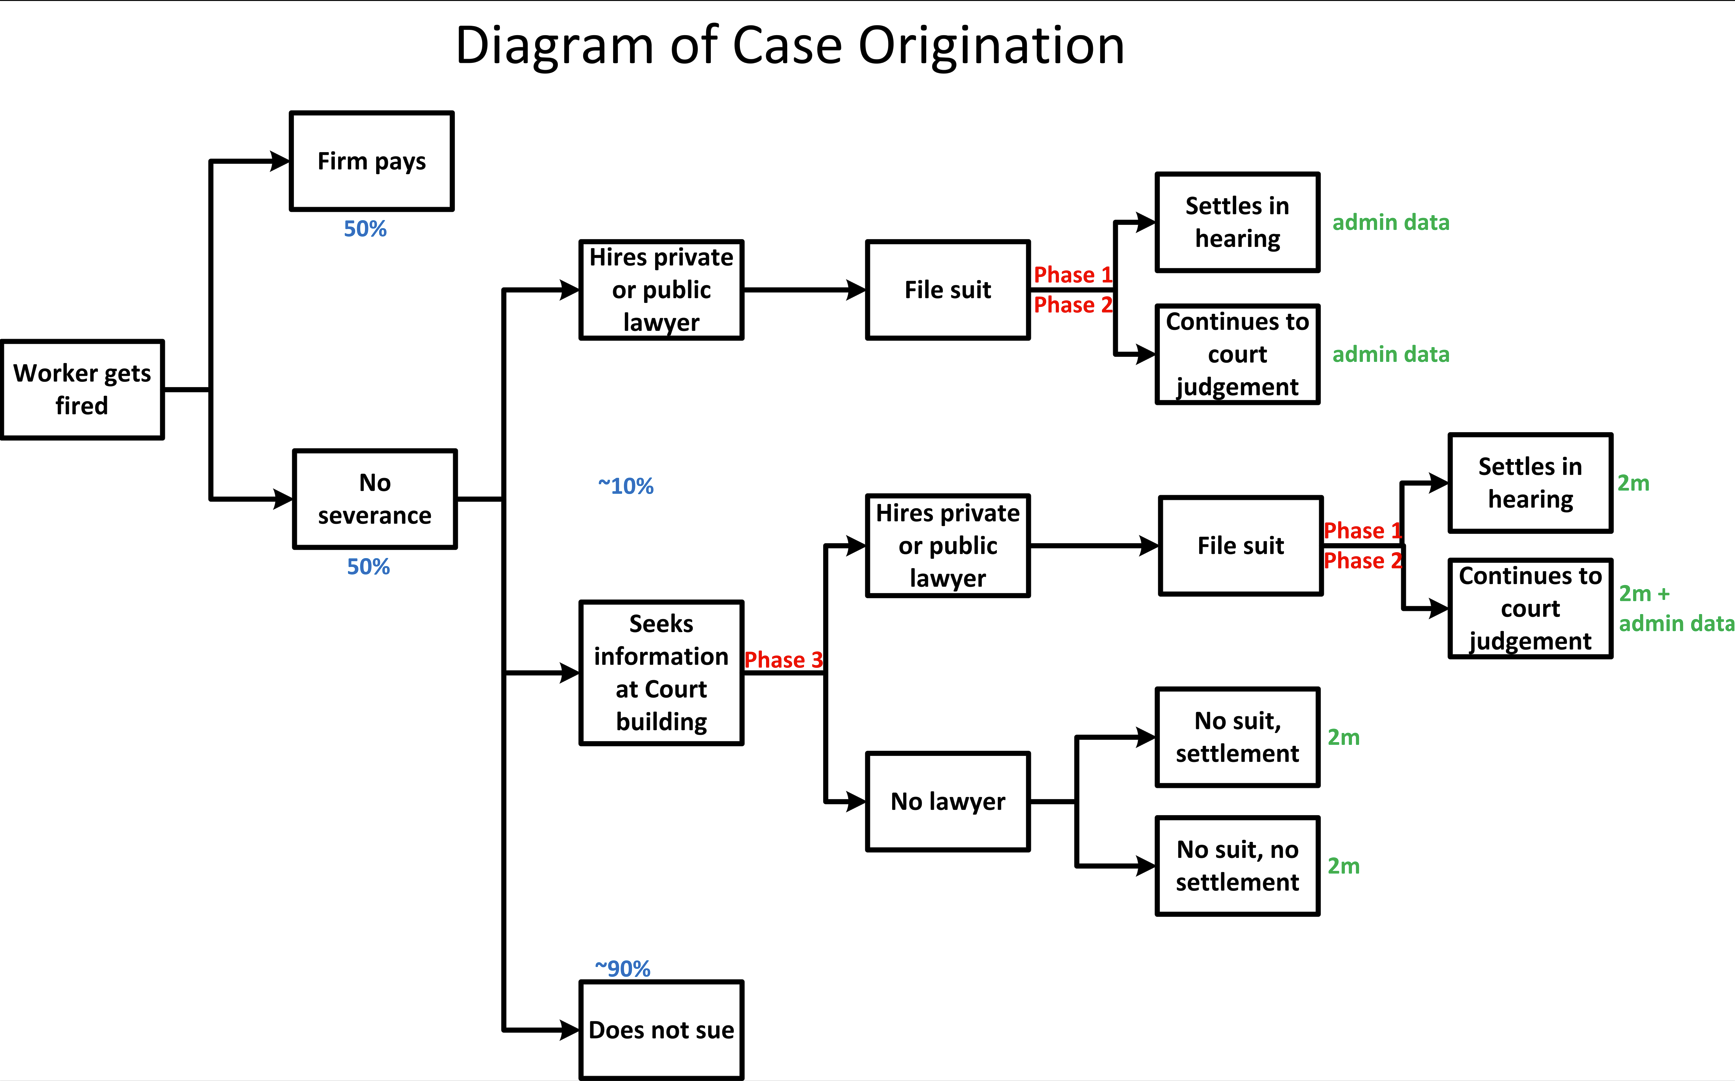
\includegraphics[width=0.9\textwidth]{paper/Figures/Diagram_Case_Origination_.png}
%         \end{center}

%     \label{stylized_representation}
% %\begin{figurenotes}
%     \scriptsize
% \textit{Notes:} This figure is a stylized representation of the process that casefiles follow in Mexico City's Labor Court.  
% %\end{figurenotes}    
% \end{figure}

\begin{figure}[!ht]
 \caption{Calculator Treatment Format (example) - Phase 2}
    \begin{center}
        \begin{subfigure}{0.49\textwidth}    
        \caption{Plaintiff}
             \centering
             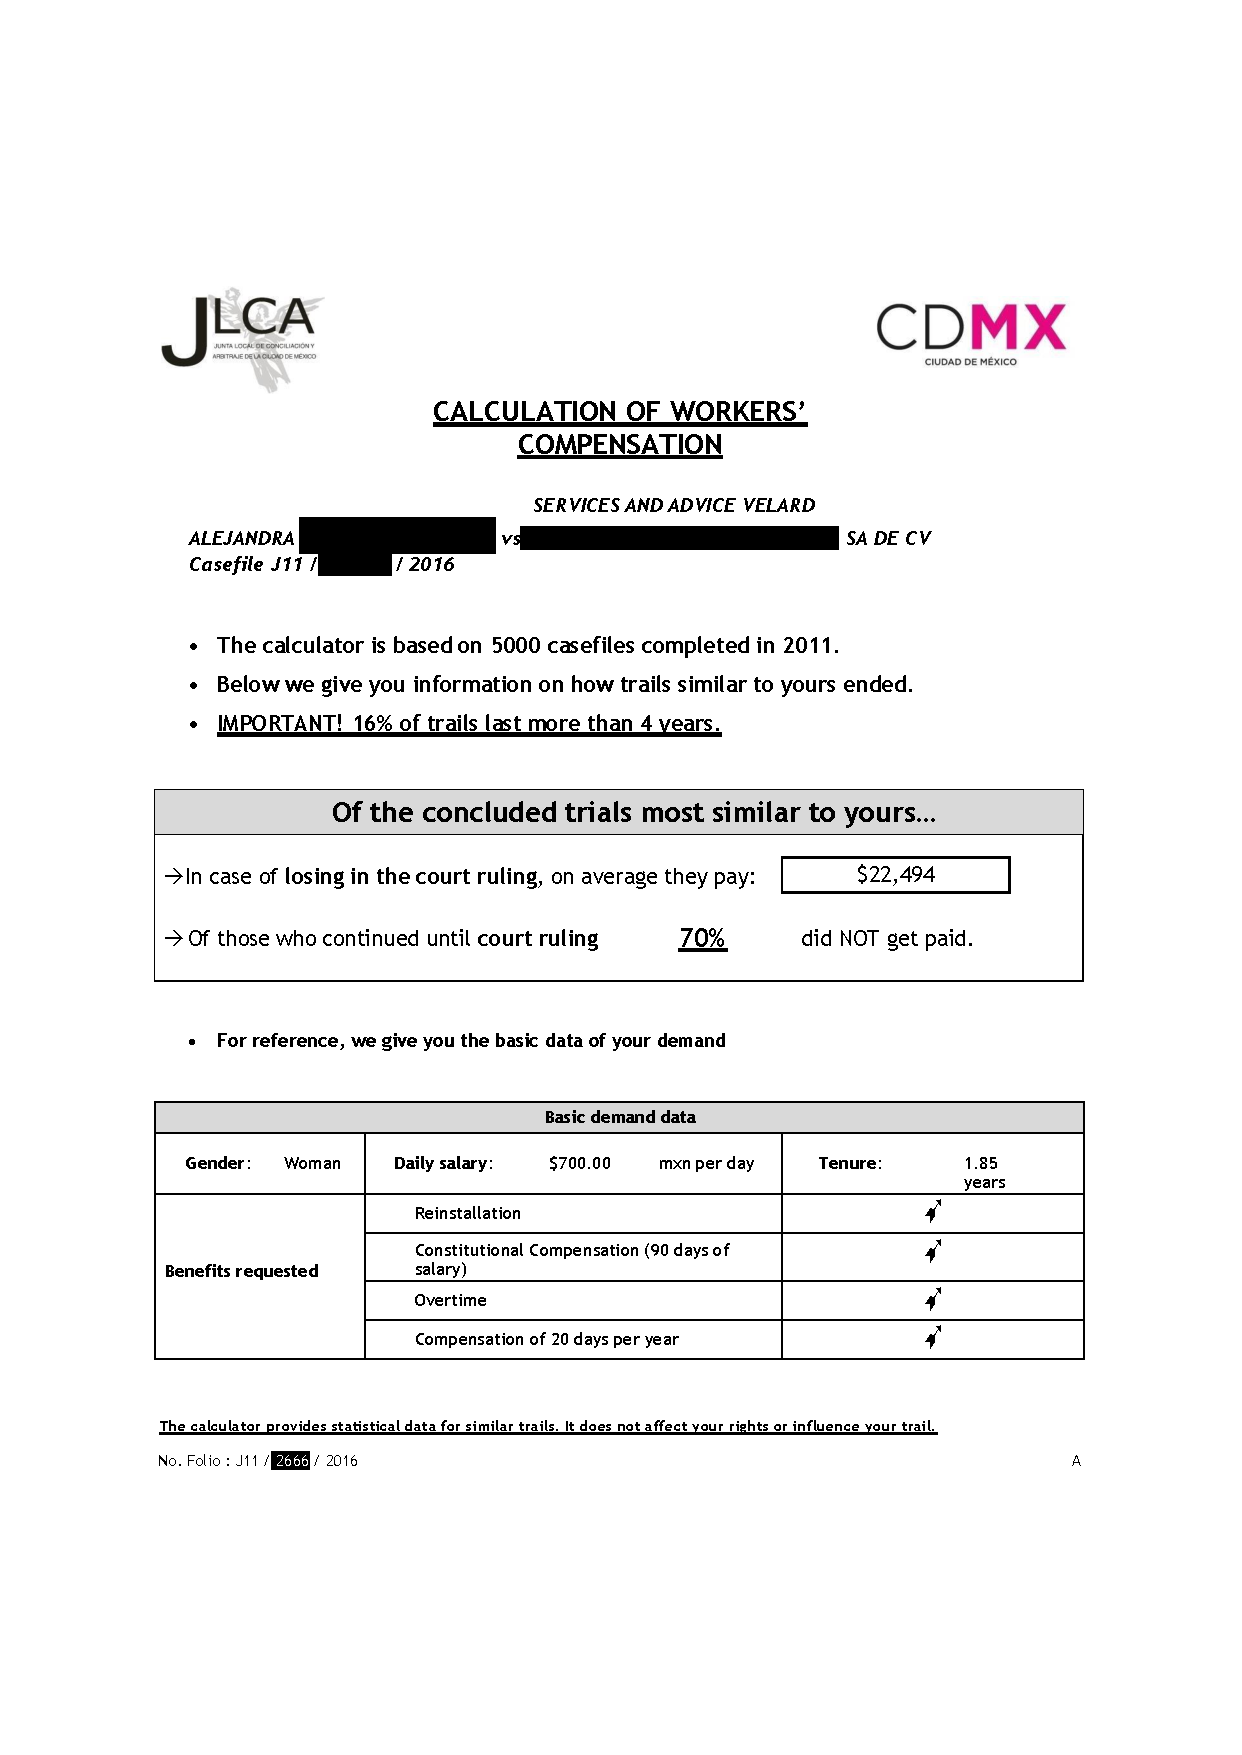
\includegraphics[width=1\textwidth]{calctreat_p2_act.pdf}
     \end{subfigure}
     \begin{subfigure}{0.49\textwidth}
     \caption{Defendant}
     \centering
         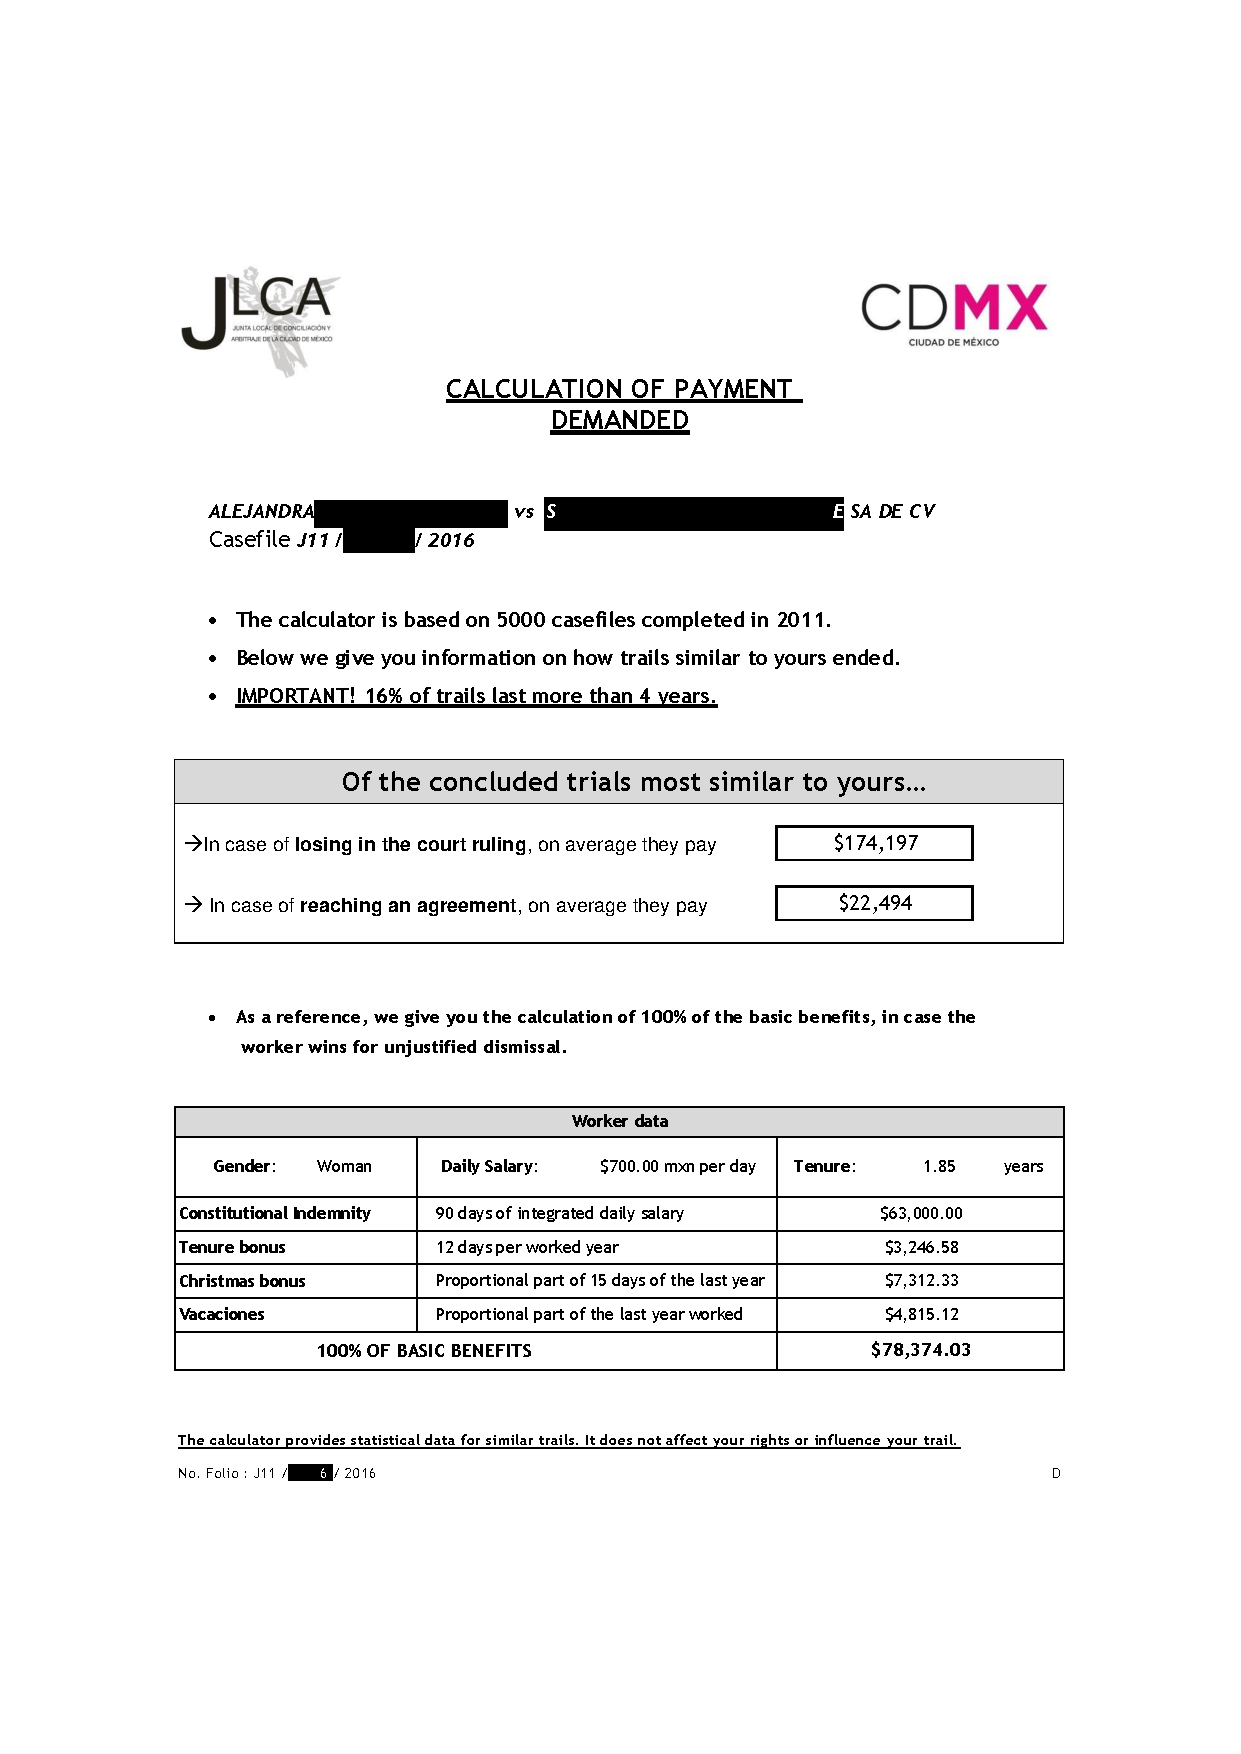
\includegraphics[width=1\textwidth]{calctreat_p2_dem.pdf}
      \end{subfigure}
        \end{center}
           
    \label{calc_template_p2}
% \begin{figurenotes}
    \scriptsize
\textit{Notes:} The figure shows examples of the calculator treatment used in phase 2. The left panel format was given to the plaintiff / dismissed worker and the right panel format to the defendant. The calculator shows two numbers: first, for cases with similar characteristics that settled, the average amount obtained in settlement; second, each party's contingency in case they did not settle and proceeded to a judge's ruling. This is the likelihood of not obtaining any payment for the plaintiff and the recovery amount conditional on positive recovery for the defendant. As in phase 1, parties were told that this information comes from a statistical exercise based on completed historical cases, and that it gives average prediction based on variables of the initial lawsuit described in the calculator treatment.
% \end{figurenotes}
\end{figure}

\begin{figure}[!ht]
     \caption{Calculator Treatment Format (example) - Phase 3}
   \label{calc_template_p3}
   \begin{center}
       \scriptsize
        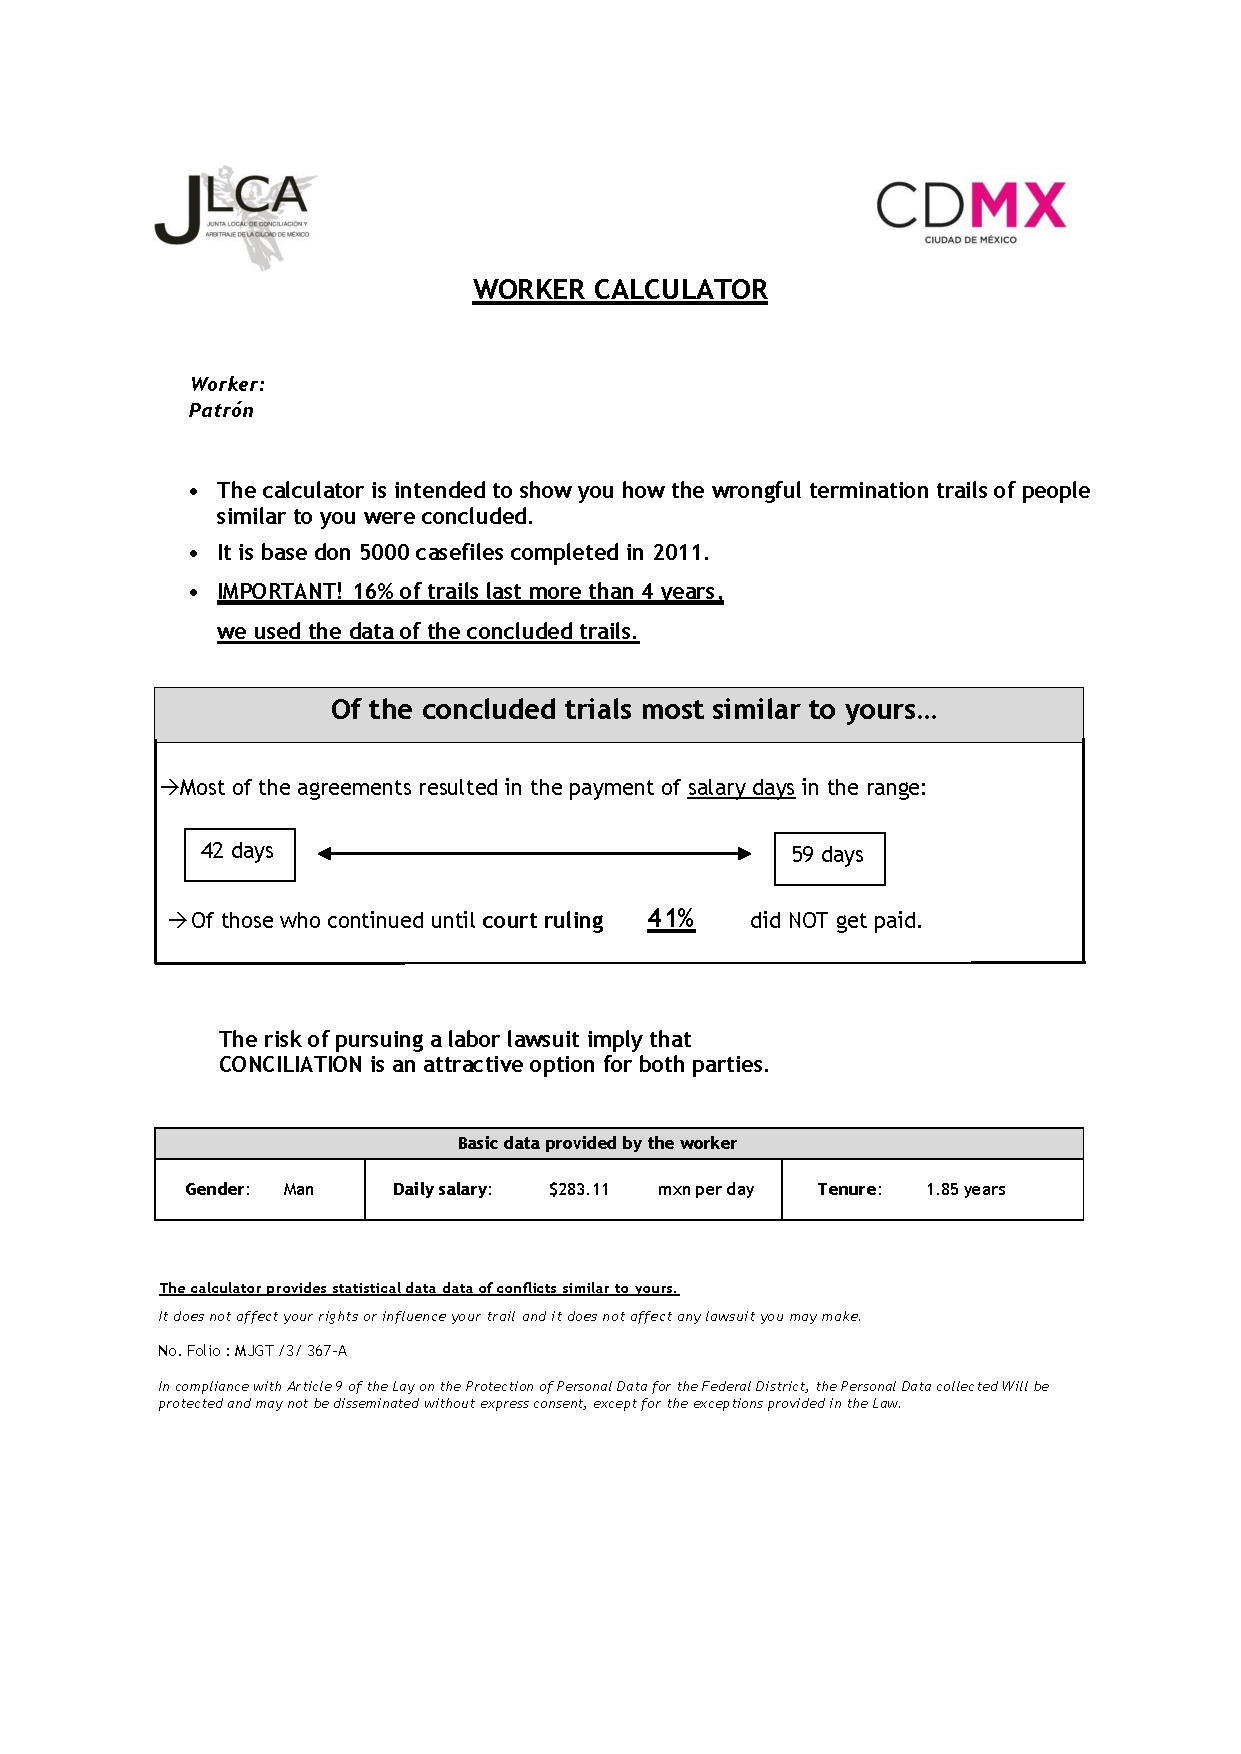
\includegraphics[width=0.5\textwidth]{paper/Figures/P3Treatments.pdf}
    \end{center}
           
 
% \begin{figurenotes}
    \scriptsize
\textit{Notes:} The figure shows an example of the calculator treatment provided to dismissed workers in phase 3. The calculator shows the inter-quartile range of settlement amounts expressed as the number of days paid and the percentage of cases continuing to court judgment where the plaintiff recovered nothing. The information provided is specific to the worker's characteristics. As in phases 1 and 2, parties were told that this information comes from a statistical exercise based on completed historical cases, and that it gives average prediction based on variables of the initial lawsuit described in the calculator treatment.
% \end{figurenotes}
\end{figure}
%\begin{figure}[!ht]
%    \caption{Prob plaintiff correctly knows what is in the lawsuit}
%    \label{knowledge_private}
%   \begin{center}
%        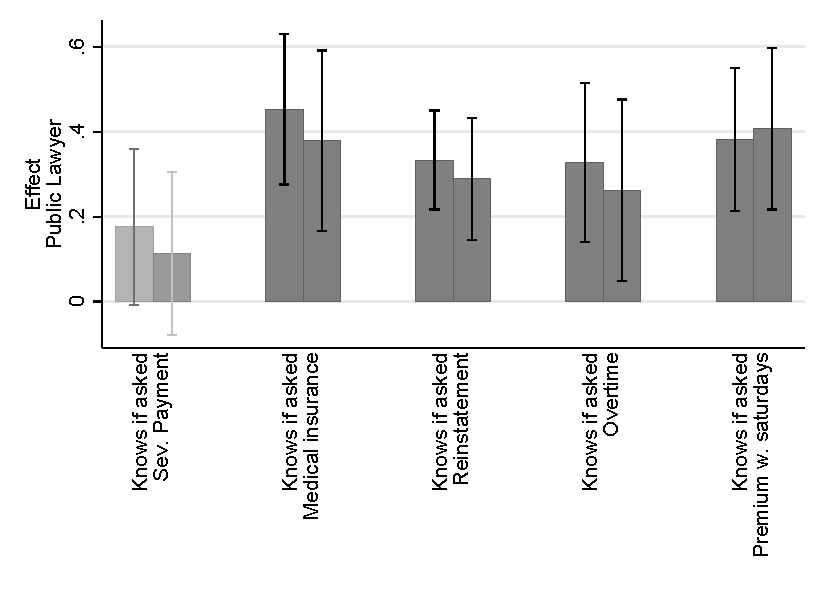
\includegraphics[width=0.8\textwidth]{knowledge_law_graph.pdf}
%        \end{center}
%        {\scriptsize \textit{Notes:} We regress a dummy variable indicating the plaintiff correctly answered a question about the contents of her case against a variable indicating the plaintiff is represented by a public lawyer. Each pair of bars shows the coefficient from the regression on the case characteristic shown in the label on the $x$ axis. In each pair, the left-hand bar is the coefficient from a regression without any control variables and the right-hand bar is the coefficient from a regression including the six basic case controls. The whisker lines represent the 95 \% confidence limits. The data indicate that clients of public lawyers are significantly more knowledgeable about the contents of their cases than are clients of private lawyers for four of the five case characteristics. 
        
        %\textit{Do File: } \texttt{knowledge\_law\_graph.do}
%        }
%\end{figure}

\begin{figure}[!ht]
\caption{Distribution of Amount Collected, by Type of Lawyer}
    \begin{center}
        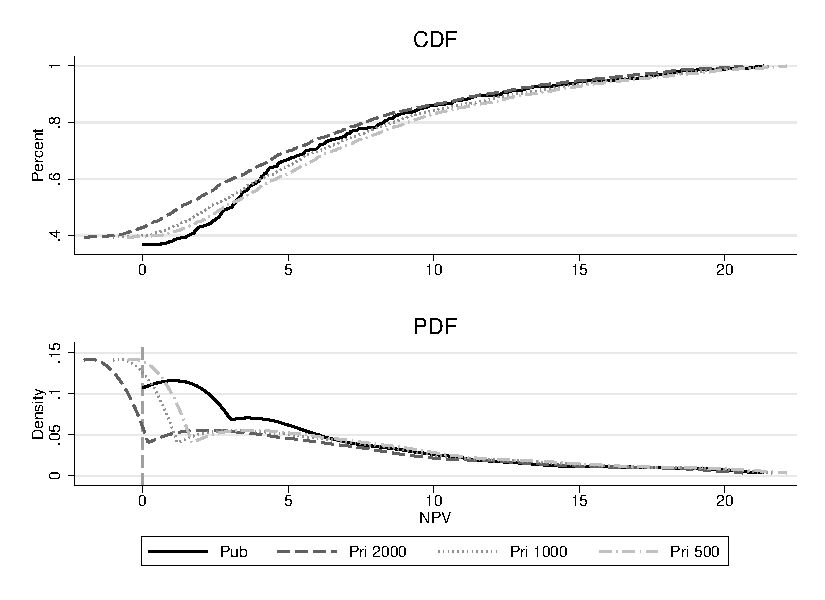
\includegraphics[width=0.9\textwidth]{cdf_pdf_value_claims.pdf}
        \end{center}
    \label{cdf_value_claims}
% \begin{figurenotes}
    \scriptsize
\textit{Notes:} This Figure uses the historical data to show cumulative distributions and densities of the amount received in the historical data. It uses all casefiles endings (court ruling, settlements, drop and expiry). Amounts on the x-axis are in thousand pesos and brought to present value to the time of suing, with a monthly interest rate of 3.43. Since we care about what the worker actually receives, when they use a private lawyer we subtract a 30\% of the recovery and the initial filing feel. The graph shows outcomes for three different initial fees (indicated in the legend): MXN\$2,000 pesos, MXN\$1,000 pesos, and MXN\$500 pesos. The modal fee in the survey data is MXN\$2,000 pesos. To the left of the vertical line at zero the worker loses money (from the initial fee). The figure indicates that there are a large fraction of cases where the worker has a negative net recovery.
    %{\scriptsize \textit{Do file: } \texttt{Fig2_cdf_value_claims_rep.do}}
% \end{figurenotes}    
\end{figure}

\begin{figure}[!ht]
    \caption{Subjective expectation minus prediction - Phase 1}
    \label{Figure_overconfidence_exp}
    \begin{center}
    \begin{subfigure}{0.45\textwidth}
        \caption{Employee}
        \centering
        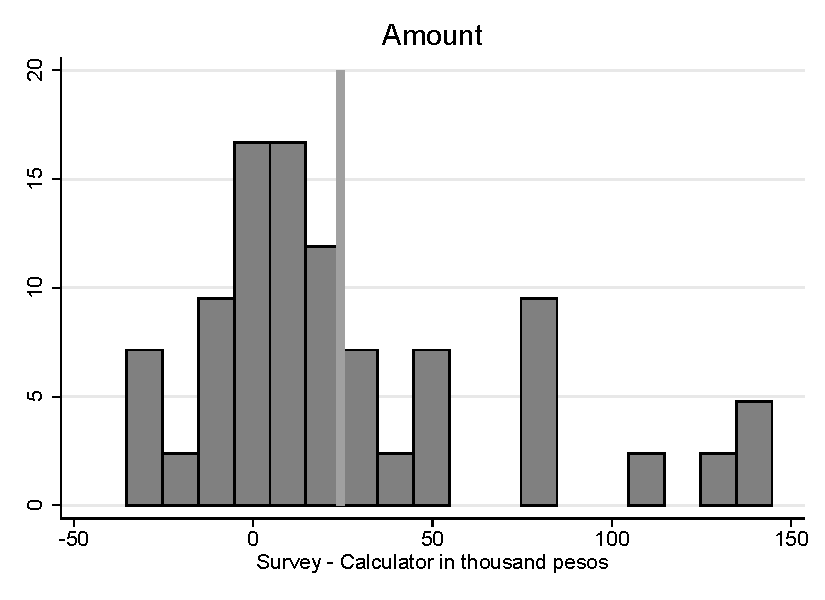
\includegraphics[width=\linewidth]{diff_amt_e.pdf}
    \end{subfigure}
    \begin{subfigure}{0.45\textwidth}
        \centering
        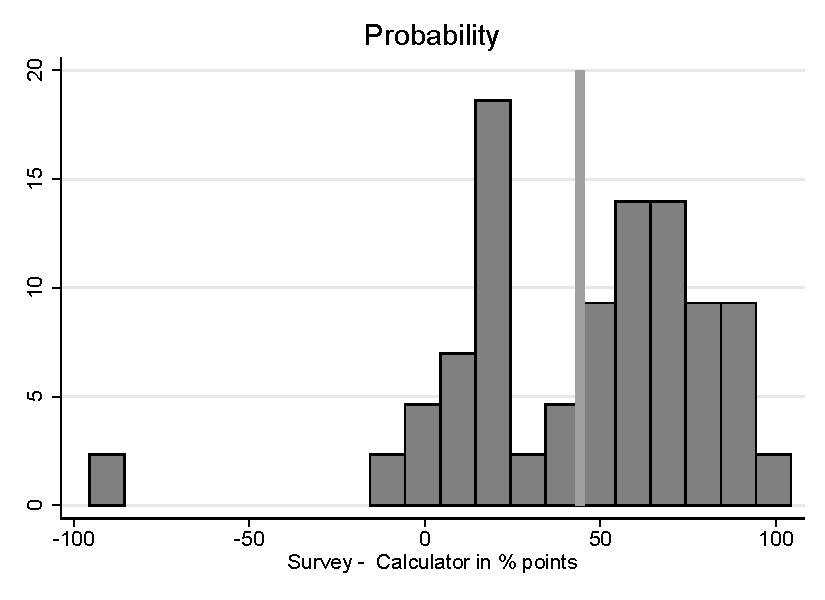
\includegraphics[width=\linewidth]{diff_prob_e.pdf}
        \end{subfigure}
        \begin{subfigure}{0.45\textwidth}
            \caption{Employee's Lawyer}
            \centering
            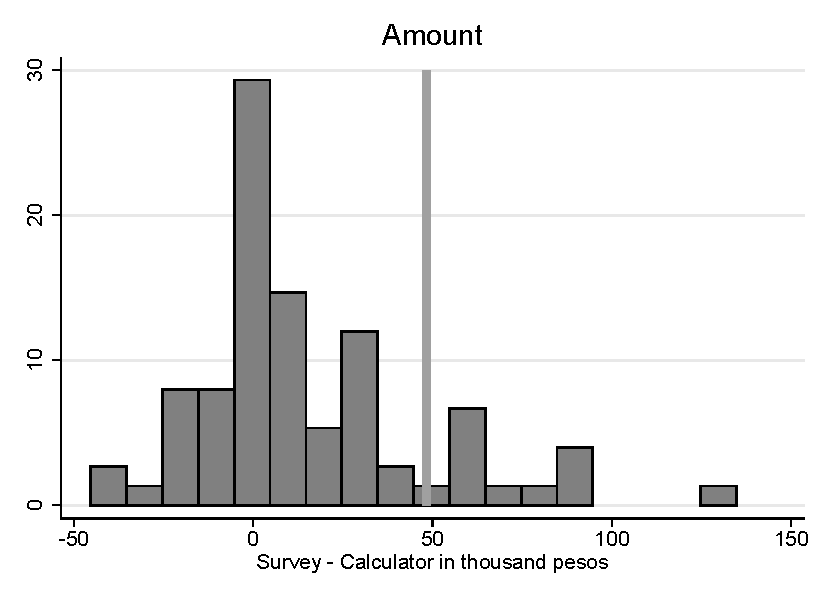
\includegraphics[width=\linewidth]{diff_amt_el.pdf}
    \end{subfigure}
    \begin{subfigure}{0.45\textwidth}
        \centering
        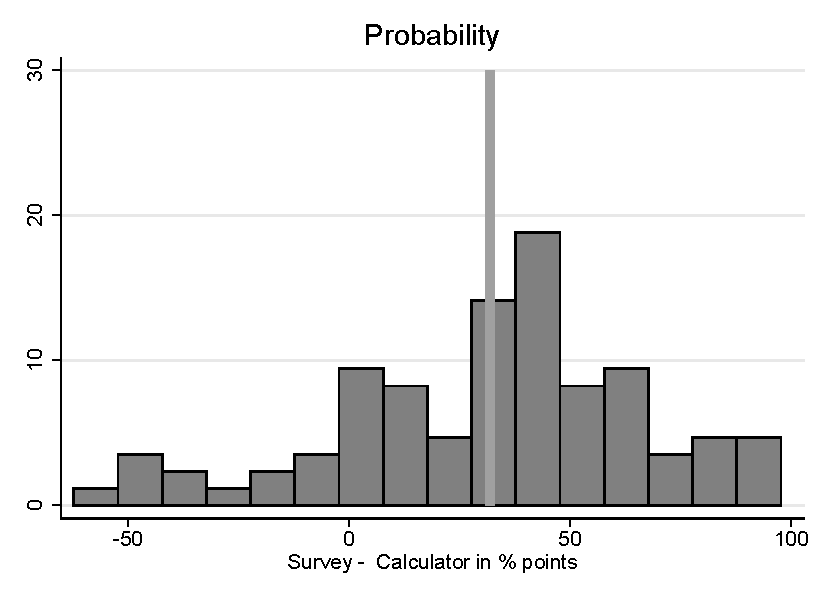
\includegraphics[width=\linewidth]{diff_prob_el.pdf}
    \end{subfigure}
    \begin{subfigure}{0.45\textwidth}
        \caption{Firm's Lawyer}
        \centering
        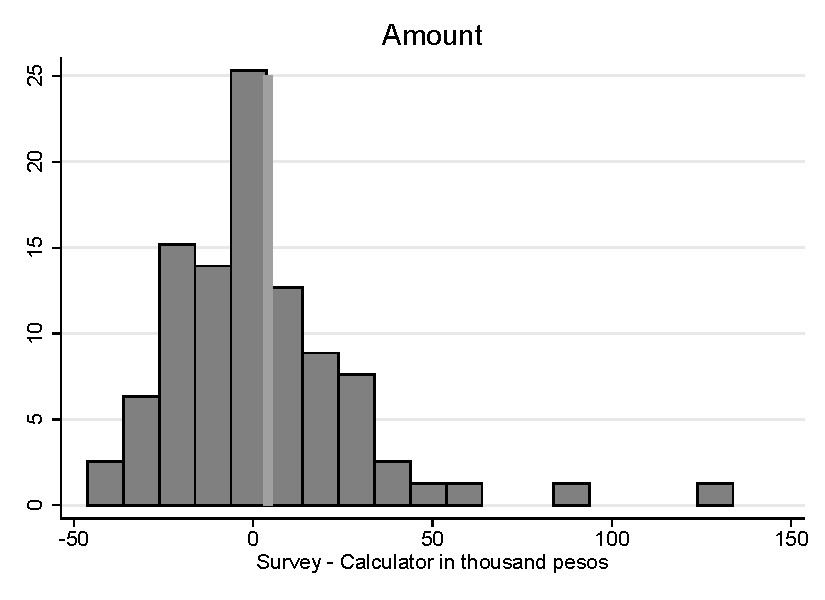
\includegraphics[width=\linewidth]{diff_amt_fl.pdf}
        \end{subfigure}
        \begin{subfigure}{0.45\textwidth}
            \centering
            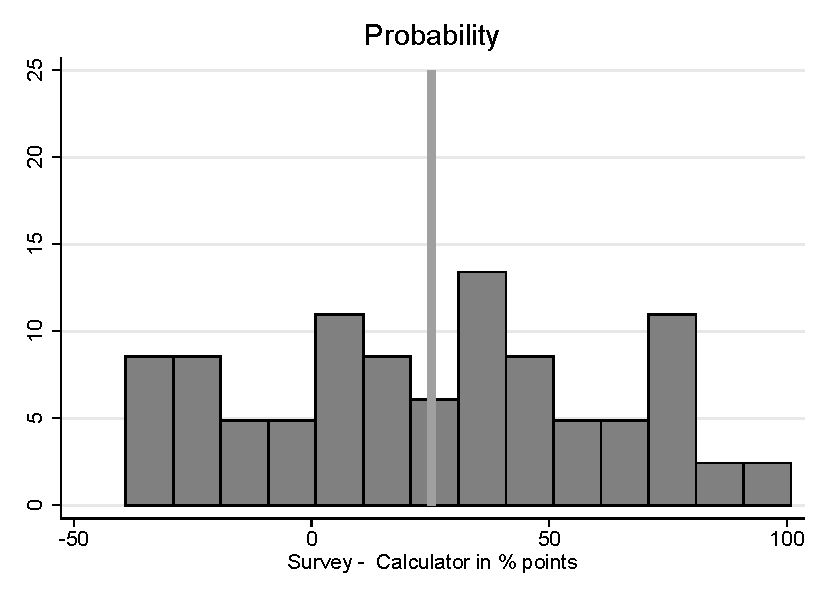
\includegraphics[width=\linewidth]{diff_prob_fl.pdf}   
    \end{subfigure}        
    \end{center}
      \scriptsize \textit{Notes:} Difference in thousand pesos for amounts (panel on left) and percentage points for probabilities (panel on right) from what the subject expects vs. what our models predict. Note how, for Employee and employee lawyer, the distribution for amounts is much more skewed to the right than for firm lawyers. This is only natural, since the former are thinking about expected wins and the latter about expected losses. 
    %   \scriptsize{ \textit{Do file: }  \texttt{oc\_comparison\_B.do}}
\end{figure}

\begin{figure}[!ht]
    \caption{Settlement Amount vs. Calculator}
        \label{RatioCalculator_Settlements}
    \begin{center}
        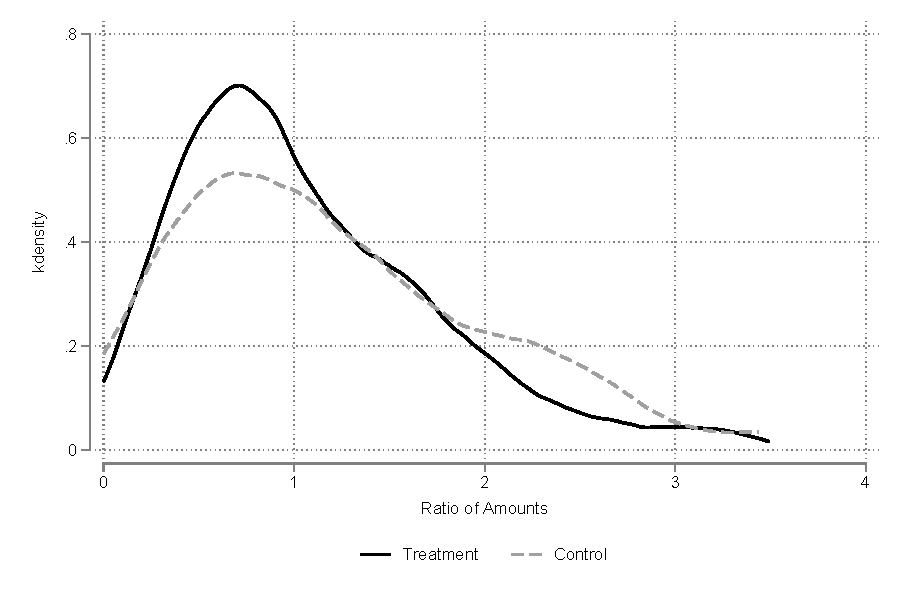
\includegraphics[width=0.6\textwidth]{paper/Figures/kdensityRatio.pdf}
         \end{center}
              \scriptsize
             \textit{Notes:} This figure presents the distribution of actual settlement amount over the calculator prediction. Data are truncated at the 99th percentile to compress the scale.
        %\textit{Do file: } \texttt{ratioGananciaConvenio.do}   
\end{figure}

\begin{figure}[!ht]
    \caption{Outcomes when Plaintiff was Present, by Treatment}
    \label{OutcomesByTreatment}
       \begin{center}
   \begin{subfigure}{0.45\textwidth}
        \caption{Phase 1}
        \centering
        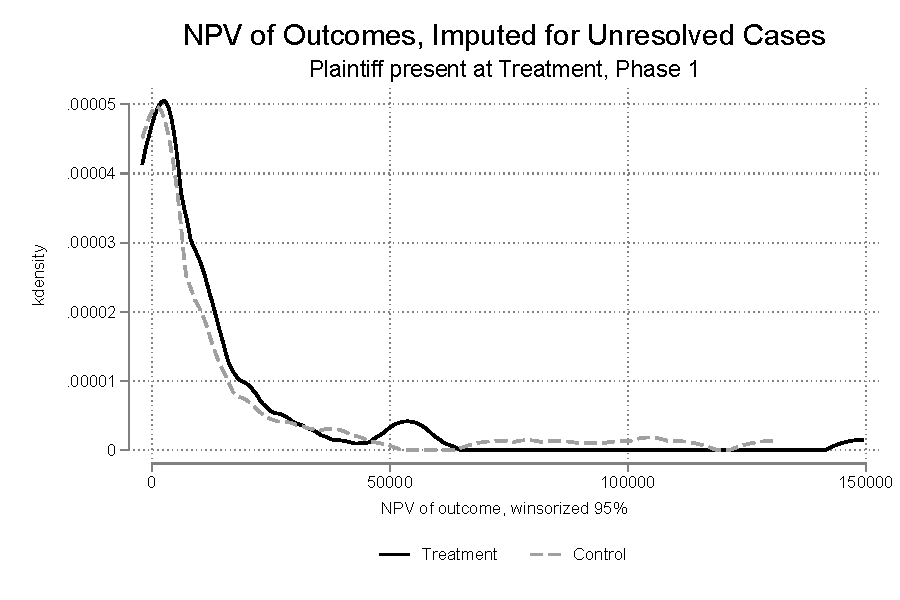
\includegraphics[width=\linewidth]{paper/Figures/OutcomesByTreatment_P1.pdf}
    \end{subfigure}
   \begin{subfigure}{0.45\textwidth}
        \caption{Phase 2}
        \centering
        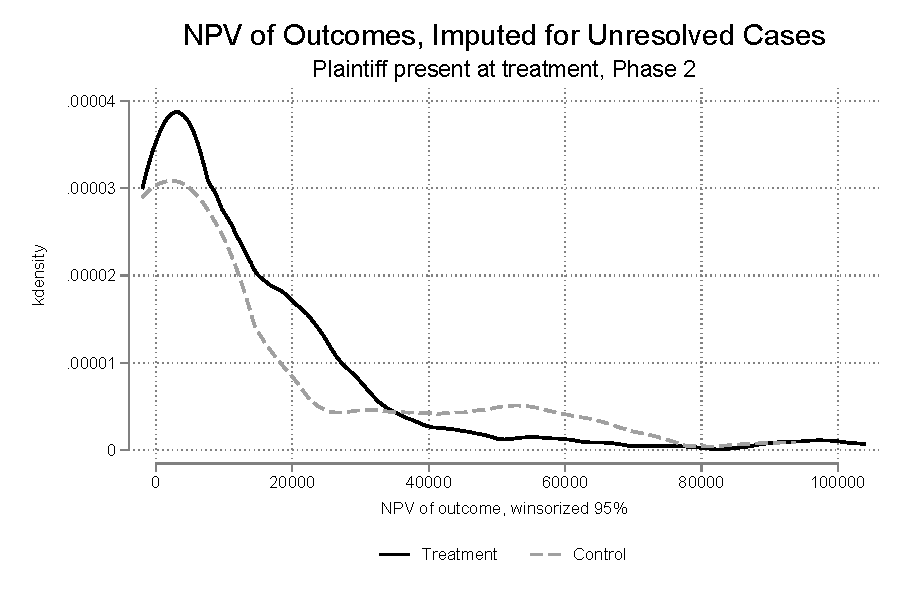
\includegraphics[width=\linewidth]{paper/Figures/OutcomesByTreatment_P2.pdf}
    \end{subfigure}
 
   
   \end{center}
      \scriptsize \textit{Notes:} This figure shows the kernel density of the NPV of the amount awarded by treatment and phase of the intervention. NPV is discounted at an annual rate of 50 percent and the value of unresolved cases is imputed from the calculator prediction for outcome by court judgment. Data are winsorized at the 95th percentile.
    %   \scriptsize{ \textit{Do file: }  \texttt{followup2020_newSpecificationitt_both}}
\end{figure}

\begin{figure}[!ht]
    \caption{Calculator Predictions for Plaintiff Court Judgment, By Phase}
    \label{Unresolved_Court_ByPhase}
       \begin{center}
   \begin{subfigure}{0.45\textwidth}
        \caption{Phase 1}
        \centering
        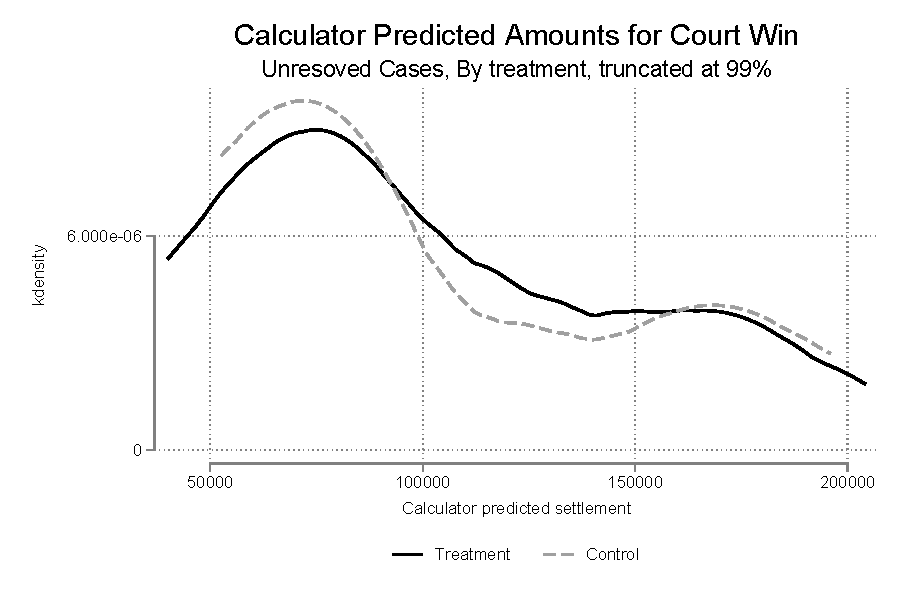
\includegraphics[width=\linewidth]{paper/Figures/Calculator_CourtWin_Unresolved_P1.pdf}
    \end{subfigure}
   \begin{subfigure}{0.45\textwidth}
        \caption{Phase 2}
        \centering
        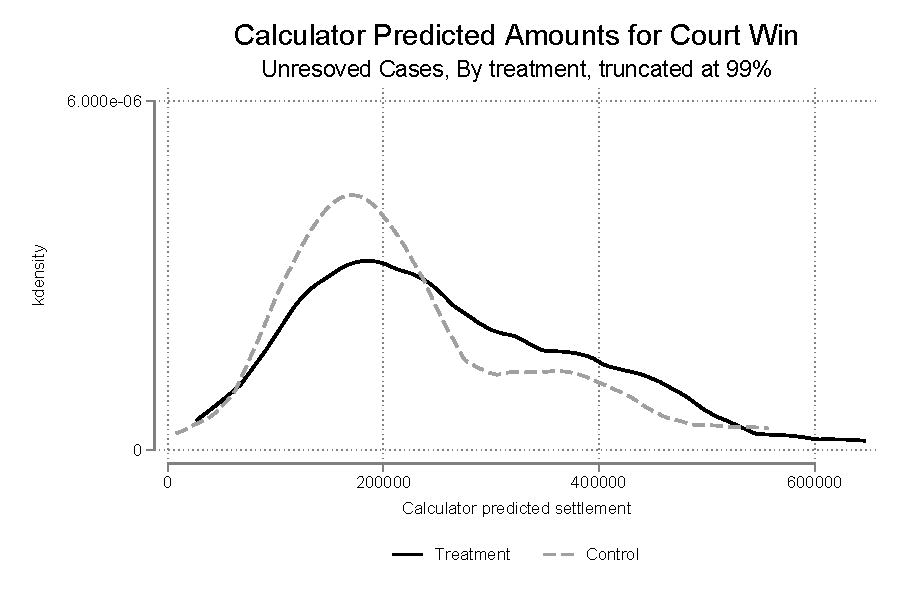
\includegraphics[width=\linewidth]{paper/Figures/Calculator_CourtWin_Unresolved_P2.pdf}
    \end{subfigure}
 
   
   \end{center}
      \scriptsize \textit{Notes:} This figure presents the calculator prediction for amount recovered conditional on the plaintiff winning a court judgment, for treatment and control cases that were unresolved as of 2020. The cases in phase 1 and phase 2 are shown separately.  Data are truncated at the 99th percentile to compress the scale.
    %   \scriptsize{ \textit{Do file: }  \texttt{casevaluekdensitiesdo.do}}
\end{figure}

\begin{figure}[!ht]
    \caption{Information handed out in placebo test}
        \label{placebo_leaflet}
    \begin{center}
        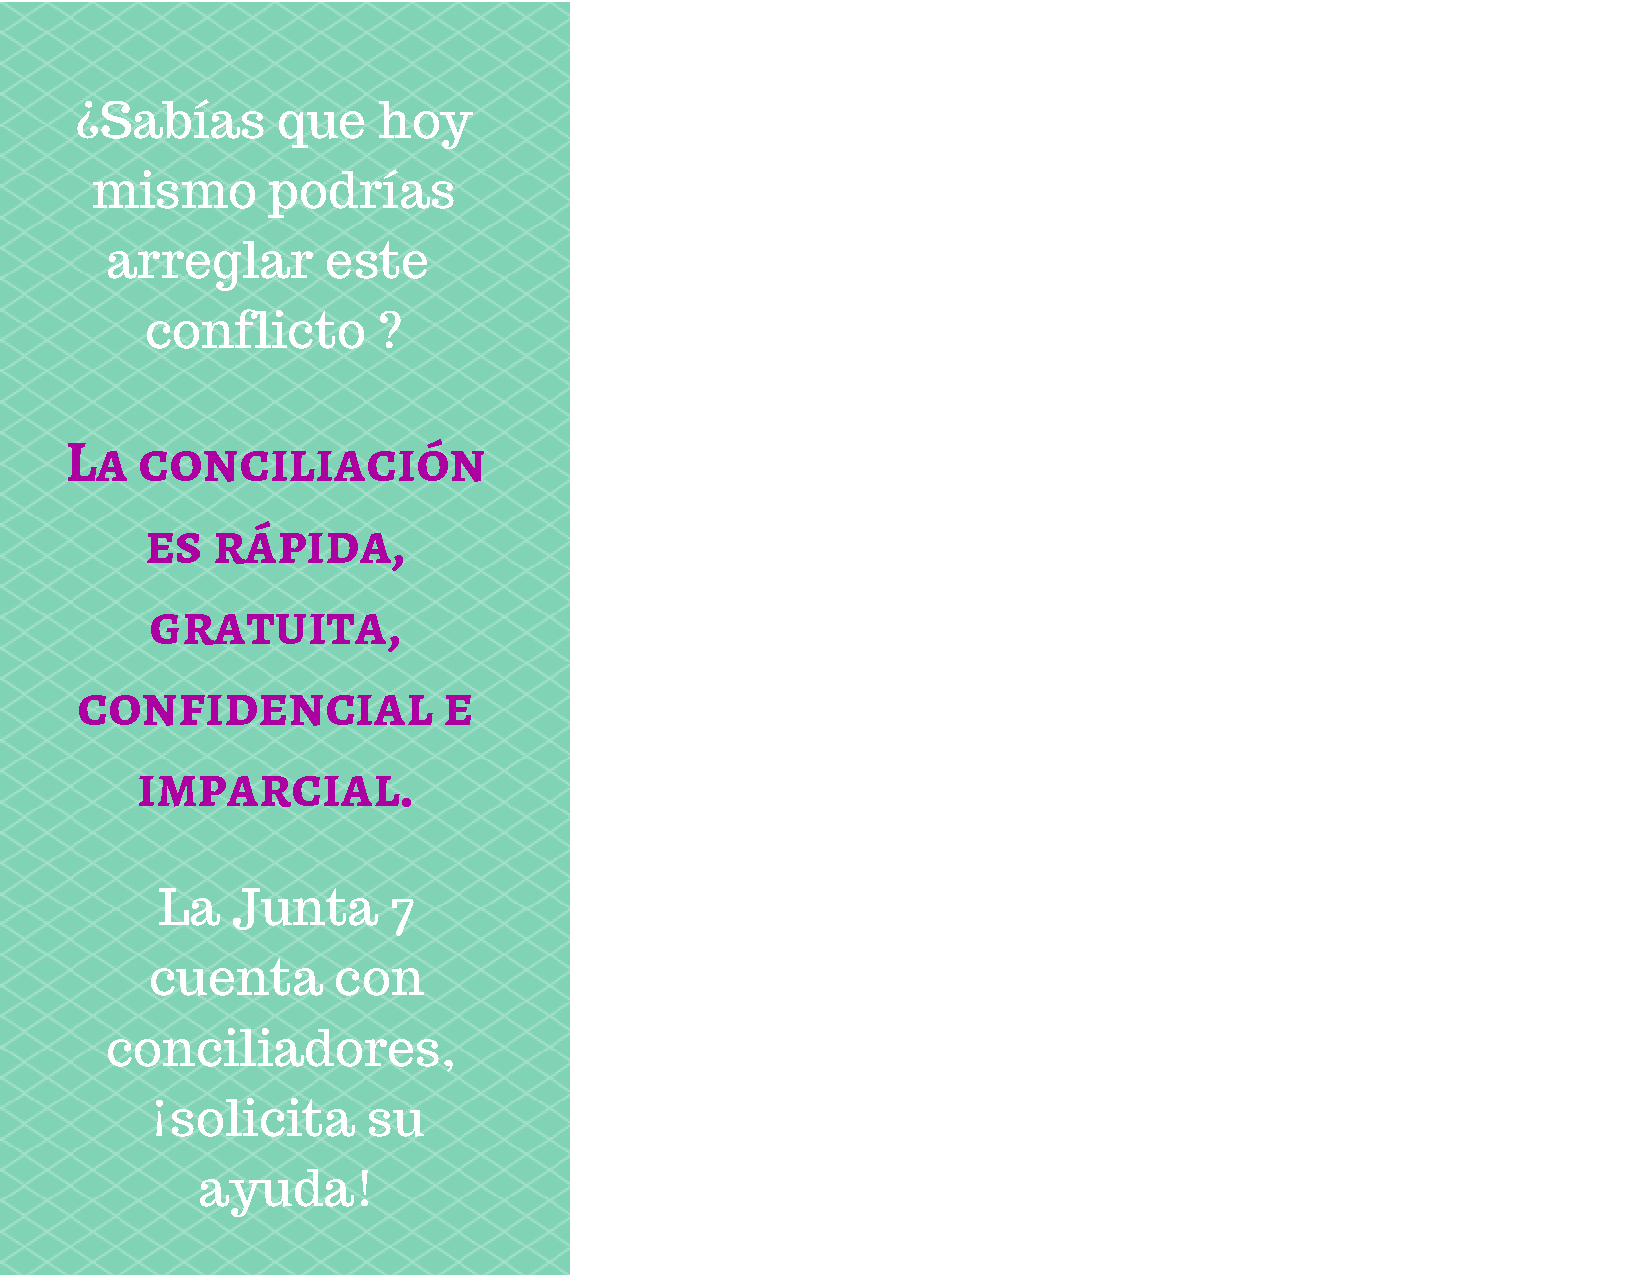
\includegraphics[width=0.4\textwidth]{placebo_information.pdf}
         \end{center}
              \scriptsize
             \textit{Notes:} This is the information brochure handed out to subjects in the placebo test. Essentially, it is a reminder of the existence of the conciliation process, which is free, confidential and unbiased.
\end{figure}

\begin{figure}[!ht]
    \caption{Discount rate for Phase 1 and MxFLS}
        \label{mxfls_comp}
    \begin{center}
        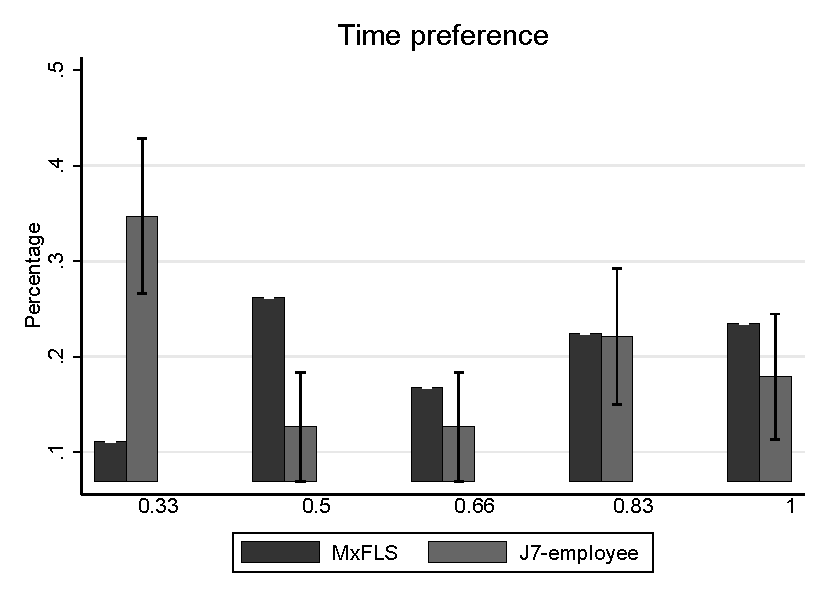
\includegraphics[width=0.6\textwidth]{discount_rate_tp_comp.pdf}
         \end{center}
              \scriptsize
             \textit{Notes:} Comparison of discount rates for Phase 1 data and survey data from the MxFLS (Mexican Family Life Survey-  a longitudinal survey in Mexico that follows individuals across rounds). In both surveys individuals are asked whether they would choose to receive \$1,000 dollars today or an array of different values in the future (\$1,200, \$1,500, \$2,000 or \$3,000 dollars). The monthly discount rate is calculated by dividing the \$1,000 dollars over the choice made by individuals.   
        %\textit{Do file: } \texttt{discount\_rate\_ph1\_mxfls.do}                   
\end{figure}

%\begin{figure}[!ht]
%    \caption{Propensity score overlap}
%        \label{ps_overlap}
%    \begin{center}
%        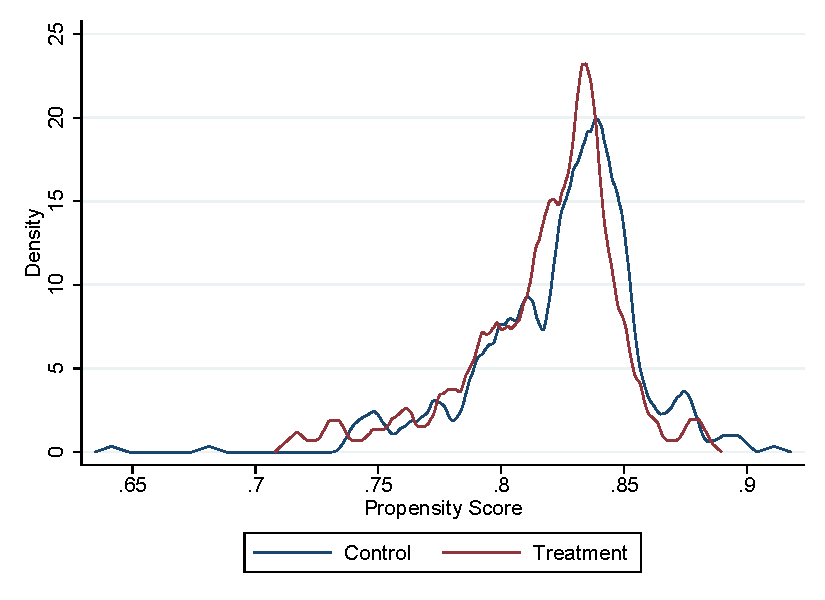
\includegraphics[width=0.6\textwidth]{ps_overlap.pdf}
%         \end{center}
%              \scriptsize
%             \textit{Notes:} The graph shows the overlap between the propensity scores after the trimming procedure suggested by \cite{CHIM_2009} and \cite{Imbens2015} when performing the analysis for table \ref{match_table}.
    %\textit{Do file: } \texttt{settlement\_conciliator\_matching.do}          
%\end{figure}



%\begin{figure}[!ht]
%    \caption{Discount rate against welfare effects}
%        \label{atematch_inrate}
%    \begin{center}
%        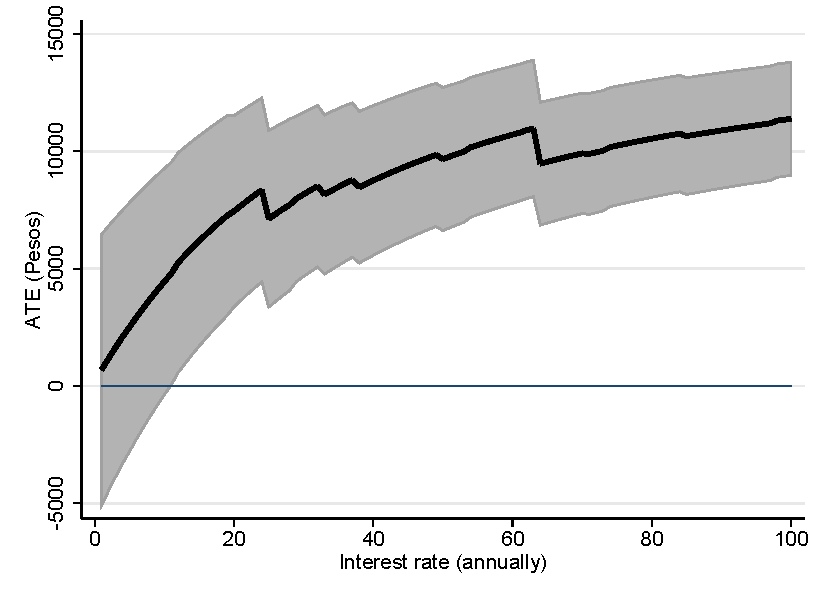
\includegraphics[width=0.6\textwidth]{atematch_intrate.pdf}
%         \end{center}
%              \scriptsize
%             \textit{Notes:} The graph shows the ATE effect of Table \ref{match_table} column (4), when using different discounting annual interest rates. 
    %\textit{Do file: } \texttt{settlement\_conciliator\_matching\_interest\_rate.do}          
%\end{figure}

%%%%%%%%%%%%%%%%%% EXPERIMENT FIGURES





\end{document}


Data from case filings in the Mexico City Labor Court show that worker dismissal lawsuits have long duration even though many have very low values. Around 40 percent of plaintiffs pay more in legal fees than they recover from their case. At the same time, survey data indicate that parties are overly-optimistic and workers are ill-informed about both the relevant law and their own cases. The patterns our data reveal are widely viewed as common across courts more generally in low- and middle-income countries. 

Results from a randomized experiment show that providing simple information on expected outcomes of the case nearly doubles the rate of settlement on the day of the treatment, and has a similar effect on resolving conflict among dismissed workers who have yet to file a case. The treatment effect is evident only when the worker is present. Both the treatment effect and the importance of the employee's presence are persistent for 42 months following the treatment. These patterns are consistent with agency issues between the plaintiff and her lawyer. We show conceptually why even a reward-sharing contract does not align incentives of the lawyer and plaintiff when the two parties assess the cost of risk differently or have different discount rates. Both of these are likely in our context. These results have important policy implications for bargaining impasses that happen in many similar contexts. The calculator is easily scalable to dispute settlement situations with a large volume of cases similar enough to allow for accurate prediction of expected outcomes. The provision of information is likely to be particularly relevant in contexts where at least one side to the dispute is not a repeat player, and hence is likely to be misinformed, such as divorce or civil cases.  

%\footnote{Moreover, the fixed filing fee may incentivize lawyers to file cases they realize have very low expected outcomes.}
One story that weaves together our results contains five elements reflecting plaintiff-lawyer agency issues: First, employees are misinformed about their entitlements and the importance of particular types of evidence. Second, employees have little access to information on the quality of lawyers, with many using low-quality informal lawyers first encountered on the steps of the court building. Third, many private lawyers inflate claims, possibly to inflate the expectations of workers to convince them to sue. Fourth, perhaps because of the second and third element, two in five plaintiffs using private lawyers realize negative net returns. Fifth, information provided to the lawyer is not transmitted to the employee. 


